\documentclass[10pt,journal]{IEEEtran}


\usepackage{graphicx}
\usepackage{amsmath,amsfonts}
\usepackage{algorithmic}
\usepackage{algorithm}
\usepackage{array}
\usepackage[caption=false,font=normalsize,labelfont=sf,textfont=sf]{subfig}
\usepackage{mathtools}
\usepackage{textcomp}
\usepackage{stfloats}
\usepackage{url}
\usepackage{verbatim}
\usepackage{cite}
\usepackage{multirow}
\usepackage{colortbl}
\hyphenation{op-tical net-works semi-conduc-tor IEEE-Xplore}
% updated with editorial comments 8/9/2021



\usepackage{amsthm}
\usepackage{amssymb}
\usepackage{booktabs}
\usepackage{color}
\usepackage{multirow}
%\usepackage[noend]{algpseudocode}
%\myexternaldocument{main}
%\externaldocument[I-]{main}
\DeclareMathOperator{\Fix}{Fix}
\DeclareMathOperator{\lev}{lev}
\DeclareMathOperator{\prox}{prox}
\DeclareMathOperator{\diag}{diag}
\DeclareMathOperator{\dom}{dom}
\DeclareMathOperator{\inter}{int}
\DeclareMathOperator{\cone}{cone}
\DeclareMathOperator{\rank}{rank}
\DeclareMathOperator{\vecop}{vec}
\DeclareMathOperator{\sgn}{sgn}
\newcommand{\argmax}{\mathop{\mathrm{argmax}}\limits}
\newcommand{\argmin}{\mathop{\mathrm{argmin}}\limits}
\newcommand{\minimize}{\mathop{\mathrm{Minimize}}\limits}

\theoremstyle{plain}
\newtheorem{lem}{Lemma}
\newtheorem{thm}{Theorem}


\def\etal{\textit{et al.}}

\def\Order#1{\mathcal{O}(#1)}

\def\InnerProduct<#1>{\langle #1 \rangle}
\def\MatrixBrackets[#1]#2{\lbrack #1 \rbrack_{#2}}
\def\AlgoLfloor#1{\left\lfloor #1 \right}
\def\MatrixIdentity{\mathbf{I}}
\def\MatrixZero{\mathbf{O}}
\def\OpNorm#1{\| #1 \|_{\mathrm{op}}}
\def\OpNormSq#1{\| #1 \|_{\mathrm{op}}^{2}}

\def\llHTV{{l_{0}\text{-}l_{1}\text{HTV}}}

\def\RealSpace#1{\mathbb{R}^{#1}}
\def\SetProperLowerConvex#1{\Gamma_{0}(#1)}
\def\SetConvex{C}
\def\FuncIndicator#1{\iota_{#1}}

\def\Projection#1{P_{#1}}


% General variables
\def\FuncOne{f}
\def\FuncTwo{g}
\def\NumVarOne{N}
\def\NumVarTwo{M}
\def\VarOne{\mathbf{x}}
\def\VarTwo{\mathbf{y}}
\def\MatrixOne{\mathbf{X}}
\def\ElementOne#1{x_{#1}}
\def\IndexOne{i}


% HSI and related 
\def\HSIClean{\mathbf{u}}
\def\HSIObsv{\mathbf{v}}
\def\NoiseSparse{\mathbf{s}}
\def\NoiseGauss{\mathbf{n}}
\def\NoiseStripe{\mathbf{t}}

\def\ResHSIClean{\HSIClean^{'}}
\def\ResNoiseSparse{\NoiseSparse^{'}}
\def\ResNoiseStripe{\NoiseStripe^{'}}

% \def\NumPixel{N}
\def\NumAll{N}
\def\NumVert{N_{1}}
\def\NumHori{N_{2}}
\def\NumBand{N_{3}}



\def\NumSingularValue{Q}


\def\IndexAlg{t}

% 2.1 Notation
\def\NotationVector{\mathbf{x}}
\def\NotationMatrix{\mathbf{X}}
\def\NotationScalar{x}
\def\NotationNumDim{N}
\def\NotationIndex{n}

% 2.2 Proximal Tools
\def\FuncProx{\FuncOne}
\def\IndexProx{\gamma}
\def\VarProxOne{\VarOne}
\def\VarProxTwo{\VarTwo}
\def\NumVarProx{\NumVarOne}
\def\ScalarProx{\delta}
\def\MatrixProx{\mathbf{G}}
\def\Projection#1{P_{#1}}


% 2.3 P-PDS
\def\FuncPrimal#1{\FuncOne_{#1}}
\def\FuncDual#1{\FuncTwo_{#1}}
\def\VarPrimal#1{\VarOne_{#1}}
\def\VarDual#1{\VarTwo_{#1}}
\def\VarDualMatrix#1{\mathbf{Y}_{#1}}

\def\NumVarPrimal{\NumVarOne}
\def\NumVarDual{\NumVarTwo}
\def\DimVarPrimal#1{n_{#1}}
\def\DimVarDual#1{m_{#1}}
\def\IndexPrimal{i}
\def\IndexDual{j}
\def\IndexVarPrimal{k}
\def\IndexVarDual{l}

\def\LinOpPPDS#1{\mathbf{A}_{#1}}
\def\ScalarStepsize#1{\gamma_{#1}}
\def\MatrixStepsize#1{\mathbf{\Gamma}_{#1}}
% \def\ParamStepsize#1{\mathbf{\Gamma}_{#1}}
\def\ParamStepsize#1{\gamma_{#1}}
\def\ASPrimal#1{\sigma_{#1}}
\def\ASDual#1{\tau_{#1}}

% \def\OpNormUp#1{\mu_{#1}}
\def\OpNormUp#1{\xi_{#1}}

\def\ConstantRow#1{c_{1, #1}}
\def\ConstantColumn#1{c_{2, #1}}


% 2.5 Spatial Graph by GSSTV
\def\GuideImage{\HSIObsv{'}}
\def\GuideImageVec{v{'}}
\def\IndexVert{i}
\def\IndexHori{j}
\def\IndexBand{c}

\def\SpatialGraph{\mathcal{G}_{\text{sp}}}
\def\SpatialGraphEdgeSet{\mathcal{E}_{\text{sp}}}
\def\SpatialGraphWeightMat{\mathbf{W}_{\text{sp}}}
\def\IndexEdgeOne{p}
\def\IndexEdgeTwo{q}
\def\SpatialGraphEdge{e_{\IndexEdgeOne, \IndexEdgeTwo}}
\def\NumSpatialGraphEdge{|\SpatialGraphEdgeSet|}
\def\SpatialGraphWeight{w_{\SpatialGraphEdge}}
\def\ParamSpatialGraph{\sigma_{\text{sp}}}


\def\SpatialGraphIncidenceMat{\mathbf{D}}
\def\DiffOpGraphSp{\mathbf{D}_{\SpatialGraph}}



% 3.1 Weighted Spectral Difference Operator based on Spectral Graph
\def\IndexSegment{k}
\def\NumSegment{K}
\def\Segment#1{\mathcal{S}_{#1}}
\def\LabelMap{\mathbf{L}}
\def\SpectrumRep#1{\mathbf{r}_{#1}}

\def\SpectralGraph{\mathcal{G}_{\lambda}}
\def\SpectralGraphNode{\mathbf{x}_{\lambda}}
\def\SpectralGraphEdgeSet{\mathcal{E}_{\lambda}}
\def\SpectralGraphWeightMat{\mathbf{W}_{\lambda}}
\def\SpectralGraphWeight#1{w_{#1}}
\def\IndexWeight{\IndexBand}
\def\ParamSpectralGraph{\sigma_{\lambda}}

\def\DiffOpGraphBand{\mathbf{D}_{\SpectralGraph}}


% 3.2 GASSTV
\def\GASSTV{\text{GASSTV}}

\def\DiffOpVert{\mathbf{D}_{\text{v}}}
\def\DiffOpHori{\mathbf{D}_{\text{h}}}
\def\DiffOpBand{\mathbf{D}_{\lambda}}
\def\DiffOpSp{\mathbf{D}_{\text{vh}}}

\def\DiffOpVertT{\DiffOpVert^{\top}}
\def\DiffOpHoriT{\DiffOpHori^{\top}}
\def\DiffOpBandT{\DiffOpBand^{\top}}
\def\DiffOpSpT{\DiffOpSp^{\top}}


\def\DiffOpGraphSpT{\DiffOpGraphSp^{\top}}
\def\DiffOpGraphBandT{\DiffOpGraphBand^{\top}}

\def\BalanceParamOne{\omega_{1}}
\def\BalanceParamTwo{\omega_{2}}



% 3.2 HSI Denoising Problem
\def\RadiusFidel{\varepsilon}
\def\RadiusSparse{\alpha}
\def\RadiusStripe{\beta}

\def\ParamsRadius{\rho}

\def\BallFidel{B_{2, \RadiusFidel}^{\HSIObsv}}
\def\BallSparse{B_{1, \RadiusSparse}}
\def\BallStripe{B_{1, \RadiusStripe}}
\def\SetZero{\{ \mathbf{0} \}}

\def\MinRange{\underline{\mu}}
\def\MaxRange{\bar{\mu}}
% \def\MinRange{\underline{\xi}}
% \def\MaxRange{\bar{\xi}}
\def\SetRange{R_{\MinRange,\MaxRange}}

\def\OperationVec{\VarOne}
\def\OperationMatrix{\MatrixOne}
% \def\SetProb{S}
% \def\BallFidel{\SetProb_{\ell_{2}}^{(\HSIObsv, \RadiusFidel)}}
% \def\BallSparse{\SetProb_{\ell_{1}}^{(\mathbf{0}, \RadiusSparse)}}
% \def\BallStripe{\SetProb_{\ell_{1}}^{(\mathbf{0}, \RadiusStripe)}}
% \def\SetZero{\{ \mathbf{0} \}}

% \def\MinRange{\underline{\mu}}
% \def\MaxRange{\bar{\mu}}
% \def\SetRange{\SetProb_{\lbrack \MinRange,\MaxRange \rbrack}}

\def\IndexVert{i}
\def\IndexHori{j}


% 4.1 Simulated HS Image Data Experiment


\def\StanDevGauss{\sigma}
\def\RateSparse{p_{\NoiseSparse}}
\def\RateStripe{p_{\NoiseStripe}}

\def\IndexNoisy{\text{(b)}}
\def\IndexSSTV{\text{(c)}}
\def\IndexHSSTVOne{\text{(d)}}
\def\IndexHSSTVTwo{\text{(e)}}
\def\IndexllHTV{\text{(f)}}
\def\IndexGSSTV{\text{(g)}}
\def\IndexGASSTV{\text{(h)}}







\begin{document}
\bstctlcite{IEEEexample:BSTcontrol}

\title{Spatio-Spectral Structure Tensor Total Variation for Hyperspectral Image Denoising and Destriping}

% \author{Shingo Takemoto and Shunsuke Ono\thanks{This work was supported in part by JST PRESTO under Grant JPMJPR21C4, and in part by JSPS KAKENHI under Grant 22H03610, 22H00512, 20H02145, and 18H05413.}}
\author{Shingo~Takemoto,~\IEEEmembership{Student~Member,~IEEE,}
        Shunsuke~Ono,~\IEEEmembership{Member,~IEEE,}
% \thanks{Manuscript received XXX, XXX; revised XXX XXX, XXX.}%
\thanks{S. Takemoto is with the Department of Computer Science, Institute of Science Tokyo, Yokohama, 226-8501, Japan (e-mail: takemoto.s.e908@m.isct.ac.jp).}
\thanks{S. Ono is with the Department of Computer Science, Institute of Science Tokyo, Yokohama, 226-8501, Japan (e-mail: ono.s.5af2@m.isct.ac.jp).}% <-this % stops a space
\thanks{This work was supported in part by Grant-in-Aid for JSPS Fellows Grant Number JP24KJ1068 and 23KJ0912, in part by JSPS KAKENHI under Grant 22H03610, 22H00512, 23H01415, 23K17461, 24K03119, and 24K22291, and in part by JST PRESTO under Grant JPMJPR21C4, JST AdCORP under Grant JPMJKB2307, and JST ACT-X Grant JPMJAX23CJ.}}

% \author{IEEE Publication Technology,~\IEEEmembership{Staff,~IEEE,}
%         % <-this % stops a space
% \thanks{This paper was produced by the IEEE Publication Technology Group. They are in Piscataway, NJ.}% <-this % stops a space
% \thanks{Manuscript received April 19, 2021; revised August 16, 2021.}}

% The paper headers
\markboth{Journal of \LaTeX\ Class Files,~Vol.~14, No.~8, August~2021}%
{Shell \MakeLowercase{\textit{et al.}}: A Sample Article Using IEEEtran.cls for IEEE Journals}

% \IEEEpubid{0000--0000/00\$00.00~\copyright~2021 IEEE}
% Remember, if you use this you must call \IEEEpubidadjcol in the second
% column for its text to clear the IEEEpubid mark.

\maketitle

\begin{abstract}
	We propose a novel regularization function, Graph-Aided Spatio-Spectral Total Variation (GASSTV), for hyperspectral (HS) image denoising. Spatio-Spectral Total Variation (SSTV), defined using second-order spatio-spectral differences, is a widely used regularization approach that effectively captures the spatio-spectral piecewise smoothness specific to HS images, enabling robust noise removal. However, SSTV uniformly computes adjacent differences in spatial and spectral dimensions, leading to the corruption of complex spatial structures and abrupt spectral variations in HS images. To address these limitations, we incorporate spatial and spectral graphs that explicitly reflect the spatial and spectral structures into the regularization model. Furthermore, we design a framework to construct these graphs from the noisy HS image. In addition, we formulate the mixed noise removal problem as a convex optimization problem involving GASSTV and develop an efficient algorithm based on the preconditioned primal-dual splitting method to solve it. Experimental results on mixed noise removal demonstrate the superior performance of GASSTV compared with existing HS image regularization models.
\end{abstract}

\begin{IEEEkeywords}
Hyperspectral image, denoising, destriping, spatio-spectral regularization, total variation, structure tensor
\end{IEEEkeywords}


%%%%%%%%%%%%%%%%%%%%%%%%%%%%%%%%%%%%%%%%%%%%%%%%%%

\section{Introduction}
\IEEEPARstart{H}{yperspectral} (HS) images, with their rich spectral information over 100 bands, are widely applied in diverse fields such as agriculture, mineralogy, astronomy, and biotechnology~\cite{Borengasser2007HSIApplications,Grahn2007Techniques, Thenkabail2016VegetationOverview,Lu2020AgricultureOverview}. Despite their potential, HS images are contaminated with noise during acquisition, which adversely affects the performance of subsequent analyses, including anomaly detection ~\cite{Matteoli2014Anomaly, Su2022Anomaly}, classification~\cite{Ghamisi2017Classification}, and unmixing~\cite{Bioucas-Dias2012UnmixingOverview, Ma2014UnmixingOverview}. Therefore, HS image denoising is an essential preprocessing step~\cite{Shen2015DenoisingOverview, Rasti2018DenoisingOverview, Shen2022DenoisingOverview, Naganuma2022Destriping}.


For HS image denoising tasks, Spatio-Spectral Total Variation (SSTV)~\cite{Aggarwal2016SSTV} is widely known as a powerful regularization method applied in state-of-the-art methods~\cite{Fan2018SSTV-LRTF, Wang2018LRTDTV, Ince2019GLSSTV, Takeyama2020HSSTV, Wang2021l0l1HTV, Takemoto2022GSSTV, Takemoto2023S3TTV, takemoto2024spatiospectral}. SSTV effectively captures the both spatial and spectral piecewise smoothness of HS images by leveraging the $\ell_{1}$-norm of spatial differences computed after spectral ones. However, SSTV evaluates neighborhood differences uniformly, which is limited to preserve 1) complex spatial structures and 2) spectral jumps.

%In this field of HS image denoising, Spatio-Spectral Total Variation~\cite{Aggarwal2016SSTV} is widely known as a powerful regularization method that captures spatial and spectral properties on HS images, and it is also applied in state-of-the-art methods~\cite{Fan2018SSTV-LRTF, Wang2018LRTDTV, Ince2019GLSSTV, Takeyama2020HSSTV, Wang2021l0l1HTV, Takemoto2022GSSTV, Takemoto2023S3TTV, takemoto2024spatiospectral}.
%SSTV characterizes the both spatial and spectral piecewise smoothness by defining the $\ell_{1}$-norm of the spatial differences after computing spectral ones.
%However, SSTV uniformly evaluates the neighborhood differences in the vertical, horizontal, and spectral directions, which limits its ability to preserve 1) complex spatial structures and 2) spectral jumps.


% To address the spatial limitations of SSTV, Graph Spatio-Spectral Total Variation (GSSTV)~\cite{Takemoto2022GSSTV} incorporates a spatial graph-based weighted difference operator into SSTV.
% In GSSTV, a method is established to construct a spatial graph that explicitly reflects the spatial structure of the target HS image from the noisy HS image.
% By utilizing the spatial graph, GSSTV successfully captures more complex spatial structures compared to SSTV.
% However, GSSTV leaves noise in regions where the spatial graph weights are close to zero, and the spectral limitations of SSTV remain unresolved.
% Therefore, we pose the research question: can we enhance the noise removal capabilities of SSTV while preserving complex spatial structures and spectral jumps?

As a promising extension of SSTV, Graph Spatio-Spectral Total Variation (GSSTV)~\cite{Takemoto2022GSSTV} integrates a spatial graph-based weighted difference operator into SSTV, addressing challenge 1) i.e., preserving complex spatial structures.
However, GSSTV leaves residual noise in low-weight regions of the spatial graph, and does not address the spectral limitations of SSTV. Now a natural question arises: \textit{can we design a regularization method that enhances the noise removal capabilities of SSTV while capturing complex spatial structures and spectral jumps?}
%However, GSSTV leaves residual noise in low-weight regions of the spatial graph, and does not address the spectral limitations of SSTV. Now a natural question arises: \textit{can we enhance the noise removal capabilities of SSTV while preserving complex spatial structures and spectral jumps?}
%To address challenge 1) of SSTV, Graph Spatio-Spectral Total Variation (GSSTV)~\cite{Takemoto2022GSSTV} incorporates a spatial graph-based weighted difference operator into SSTV.
%By utilizing the spatial graph, GSSTV successfully captures more complex spatial structures compared to SSTV.
%However, GSSTV leaves noise in low-weight regions of the spatial graph , and does not resolve the spectral limitations of SSTV.
%Therefore, we pose the research question: can we enhance the noise removal capabilities of SSTV while preserving complex spatial structures and spectral jumps?

In this paper, we propose a novel method that incorporates both spatial and spectral graph-based TVs into SSTV, called Graph-Aided Spatio-Spectral Total Variation (GASSTV).
The main contributions of this article are listed below:
\begin{itemize}
    \setlength{\leftskip}{-10pt}
%    \item We design a novel regularization method, namely GASSTV. GASSTV integrates two weighted TVs based on spatial and spectral graphs separately from SSTV, thereby enhancing the noise removal capabilities of SSTV while capturing complex spatial structures and spectral jumps. Furthermore, we propose a robust approach to construct the spectral graph from the observed noisy HS image (Refer to GSSTV for constructing the spatial graph).
    \item We propose a novel regularization method, Graph-Aided Spatio-Spectral Total Variation (GASSTV), which incorporates spatial and spectral graph-based weighted TVs separately from SSTV. These graph-based TVs enhance the noise removal capabilities of SSTV while preserving complex spatial structures and spectral jumps. Furthermore, we robustly construct the spectral graph from the noisy HS image (Refer to GSSTV for constructing the spatial graph).
    \item We formulate the HS image denoising problem as a constrained convex optimization problem involving GASSTV. To simplify parameter tuning, we impose data fidelity and sparse noise characterization terms as constraints rather than adding them to the objective function.
    \item We develop an efficient algorithm based on Preconditioned Primal-Dual Splitting Method (P-PDS)~\cite{Pock2011PPDS, Naganuma2023PPDS} to solve our optimization problem. Unlike standard PDS~\cite{Chambolle2011PDS, Condat2013PDS}, P-PDS automatically determines appropriate stepsizes.
\end{itemize}
Finally, we demonstrate the effectiveness of GASSTV by comparing it with state-of-the-art HS image regularization methods through HS image denoising experiments.
\section{Preliminaries}
\label{sec:Preliminaries}
% \vspace{-4mm}

\subsection{Notations}
\label{subsec:Notations}
% \vspace{-2mm}
Throughout this paper, we denote vectors and matrices by boldface lowercase letters (e.g., $\NotationVector$) and boldface capital letters (e.g., $\NotationMatrix$), respectively.
We treat an HS image, denoted by $\HSIClean$ with $\NumVert$ vertical pixels, $\NumHori$ horizontal pixels, and $\NumBand$ bands.
We denote the total number of elements in the HS image by $\NumAll = \NumVert \NumHori \NumBand$.
For a matrix data $\NotationMatrix \in \RealSpace{\NumVert \times \NumHori}$, the value at the location $(\IndexPrimal, \IndexDual)$ is denoted by $[\NotationMatrix]_{\IndexPrimal,\IndexDual}$.
The $\ell_{1}$-norm and the $\ell_{2}$-norm of a vector $\NotationVector \in \RealSpace{\NotationNumDim}$ are defined as $\| \NotationVector \|_{1} := \sum_{\NotationIndex=1}^{\NotationNumDim} | \NotationScalar_{\NotationIndex} |$ and $\| \NotationVector \|_{2} := \sqrt{\sum_{\NotationIndex=1}^{\NotationNumDim} \NotationScalar_{\NotationIndex}^{2}}$, respectively, where  $\NotationScalar_{\NotationIndex}$ represents the $\NotationIndex$-th entry of $\NotationVector$.
The nuclear norm of a marix, which is the sum of all the singular values, is denoted by $\| \cdot \|_{*}$.
For an HS image $\HSIClean \in \RealSpace{\NumAll}$, let $\DiffOpVert \in \RealSpace{\NumAll \times \NumAll}$, $\DiffOpHori \in \RealSpace{\NumAll \times \NumAll}$, and $\DiffOpBand \in \RealSpace{\NumAll \times \NumAll}$ be the forward difference operators along the horizontal, vertical, and spectral directions, respectively, with the periodic boundary condition.
Here, a spatial difference operator is denoted by $\DiffOpSp := \begin{pmatrix} \DiffOpVertT & \DiffOpHoriT \end{pmatrix}^{\top} \in \RealSpace{2 \NumAll \times \NumAll}$. 
Using $\DiffOpVert$, $\DiffOpHori$, and $\DiffOpBand$, we denote the second-order spatio-spectral differences by $\DiffOpVert \DiffOpBand \HSIClean \in \RealSpace{\NumAll}$ and $\DiffOpHori \DiffOpBand \HSIClean \in \RealSpace{\NumAll}$.
Other notations will be introduced as needed.



\subsection{Proximal Tools}
\label{subsec:Prox}
In this chapter, we introduce basic proximal tools that play a central role in the optimization part of our method.
Let $\FuncProx$ be a \textit{proper lower semi-continuous convex function}.\footnote{A function $\FuncProx \: : \: \RealSpace{\NumVarProx} \rightarrow ( -\infty, \infty ]$ is called a proper lower semi-continuous convex function if $\lbrace \VarProxOne \in \RealSpace{\NumVarProx} | \FuncProx(\VarProxOne) < \infty \rbrace$ is nonempty, $\lbrace \VarProxOne \in \RealSpace{\NumVarProx} | \FuncProx(\VarProxOne) \leq \alpha \rbrace$ is closed for every $\alpha \in \RealSpace{}$, and $\FuncProx(\lambda \VarProxOne + (1-\lambda)\VarProxTwo) \leq \lambda\FuncProx(\VarProxOne) + (1-\lambda)\FuncProx(\VarProxTwo)$ for every $\VarProxOne, \VarProxTwo \in \RealSpace{\NumVarProx}$ and $\lambda \in (0, 1)$.}
Then, for $\IndexProx > 0$, the \textit{proximity operator} of $\FuncProx$ is defined by
\begin{equation}
	\label{eq:Prox}
	\prox_{\IndexProx, \FuncProx}(\VarProxOne) := \arg\min_{\VarProxTwo \in \RealSpace{\NumVarProx}} \FuncProx(\VarProxTwo) + \frac{1}{2 \IndexProx} \| \VarProxOne - \VarProxTwo \|_{2}^{2}.
\end{equation}


The \textit{Fenchel--Rockafellar conjugate function} $\FuncProx^{*}$ of the function $\FuncProx$ is defined by
\begin{equation}
	\label{eq:ConjugateFunction}
	\FuncProx^{*}(\VarProxOne) := \sup_{\VarProxTwo} \InnerProduct<\VarProxOne, \VarProxTwo> - \FuncProx(\VarTwo),
\end{equation}
where $\InnerProduct<\cdot , \cdot>$ is the Euclidean inner product.
Thanks to a generalization of Moreau's identity~\cite{Combettes2013Moreau}, the proximity operator of $\FuncProx^{*}$ is calculated as
\begin{equation}
	\label{eq:ProxConjugate}
	\prox_{\IndexProx, \FuncProx^{*}}(\VarProxOne) = \VarProxOne - \IndexProx \prox_{\frac{1}{\IndexProx} \FuncProx} \left( \frac{1}{\IndexProx} \VarProxOne \right).
\end{equation}


The indicator function of a set $\SetConvex \subset \RealSpace{\NumVarOne}$, denoted by $\FuncIndicator{\SetConvex}$, is defined as 
\begin{equation}
	\label{eq:Indicator_Function}
	\FuncIndicator{\SetConvex} (\VarOne) := 
	\begin{cases}
		0, & \mathrm{if} \: \VarOne \in \SetConvex, \\
		\infty, & \mathrm{otherwise}.
	\end{cases}
\end{equation}
The function $\FuncIndicator{\SetConvex}$ is proper lower semi-continuous convex when $\SetConvex$ is nonempty and closed convex.
The proximity operator of $\FuncIndicator{\SetConvex}$ is equivalent to the projection onto $\SetConvex$, as given by
\begin{equation}
	\label{eq:Projection}
	\prox_{\FuncIndicator{\SetConvex}} (\VarProxOne) = \Projection{\SetConvex}(\VarProxOne) := \argmin_{\VarProxTwo \in \SetConvex} \|\VarProxTwo - \VarProxOne \|_{2}.
\end{equation}


\subsection{Preconditoned Primal-Dual Splitting Method (P-PDS)}
\label{subsec:P-PDS}
The standard PDS~\cite{Chambolle2011PDS, Condat2013PDS} and P-PDS~\cite{Pock2011PPDS}, on which our algorithm is based, are efficient algorithms for solving the following generic form of convex optimization problems:
\begin{align}
	\label{prob:convex_optim_prob}
	\min_{\substack{\VarPrimal{1}, \ldots, \VarPrimal{\NumVarPrimal}, \\ 
			\VarDual{1}, \ldots, \VarDual{\NumVarDual}}} 
	& \sum_{\IndexPrimal=1}^{\NumVarPrimal} \FuncPrimal{\IndexPrimal} (\VarPrimal{\IndexPrimal}) + \sum_{\IndexDual=1}^{\NumVarDual} \FuncDual{\IndexDual} (\VarDual{\IndexDual}) \nonumber \\ 
	& \mathrm{s.t.} \:
	\begin{cases} 
		\VarDual{1} = \sum_{\IndexPrimal=1}^{\NumVarPrimal} \LinOpPPDS{1,\IndexPrimal} \VarPrimal{\IndexPrimal}, \\ 
		\vdots \\ 
		\VarDual{\NumVarDual} = \sum_{\IndexPrimal=1}^{\NumVarPrimal} \LinOpPPDS{\NumVarDual,\IndexPrimal} \VarPrimal{\IndexPrimal}, 
	\end{cases}
\end{align}
where $\FuncPrimal{\IndexPrimal} (\IndexPrimal = 1, \ldots, \NumVarPrimal)$ and $\FuncDual{\IndexDual} (\IndexDual = 1, \ldots, \NumVarDual)$ are lower semi-continuous proper convex functions, $\VarPrimal{\IndexPrimal} \in \RealSpace{\DimVarPrimal{\IndexPrimal}} \: (\IndexPrimal = 1, \dots, \NumVarPrimal)$ are primal variables, $\VarDual{\IndexDual} \in \RealSpace{\DimVarDual{\IndexDual}} \: (\IndexDual = 1, \dots, \NumVarDual)$ are dual variables, and $\LinOpPPDS{\IndexDual,\IndexPrimal} \in \RealSpace{\DimVarDual{\IndexDual} \times  \DimVarPrimal{\IndexPrimal}}$ ($i = 1, \ldots, \NumVarPrimal$, $j = 1, \ldots, \NumVarDual$) are linear operators.

These methods solve Prob.~\eqref{prob:convex_optim_prob} by the following iterative procedures:
\begin{equation}
	\label{algo:P-PDS}
	\AlgoLfloor{
		\begin{array}{l}
			\VarPrimal{1}^{(\IndexAlg+1)} 
			\leftarrow \prox_{\ScalarStepsize{1, 1}, \FuncPrimal{1}}
			\left( \VarPrimal{1}^{(\IndexAlg)} - \ScalarStepsize{1,1} \bigl( \sum_{\IndexDual=1}^{\NumVarDual} \LinOpPPDS{\IndexDual,1}^{\top} \VarDual{\IndexDual}^{(\IndexAlg)} \bigr) \right), \\
			\vdots \\
			\VarPrimal{\NumVarPrimal}^{(\IndexAlg+1)} 
			\leftarrow \prox_{\ScalarStepsize{1, \NumVarPrimal}, \FuncPrimal{\NumVarPrimal}}
			\left( \VarPrimal{\NumVarPrimal}^{(\IndexAlg)} - \ScalarStepsize{1, \NumVarPrimal} \bigl( \sum_{\IndexDual=1}^{\NumVarDual} \LinOpPPDS{\IndexDual,\NumVarPrimal}^{\top} \VarDual{\IndexDual}^{(\IndexAlg)} \bigr) \right), \\
			\VarPrimal{\IndexPrimal}^{'} = 2\VarPrimal{\IndexPrimal}^{(\IndexAlg+1)} - \VarPrimal{\IndexPrimal}^{(\IndexAlg)} \: (\forall \IndexPrimal = 1, \ldots, \NumVarPrimal), \\
			\VarDual{1}^{(\IndexAlg+1)}
			\leftarrow \prox_{\ScalarStepsize{2, 1}, \FuncDual{1}^{*}}
			\left( \VarDual{1}^{(\IndexAlg)} - \ScalarStepsize{2, 1}
			\bigl(\sum_{\IndexPrimal=1}^{\NumVarPrimal} \LinOpPPDS{1,\IndexPrimal} \VarPrimal{\IndexPrimal}^{'} \bigr) \right), \\
			\vdots \\
			\VarDual{\NumVarDual}^{(\IndexAlg+1)}
			\leftarrow \prox_{\ScalarStepsize{2, \NumVarDual}, \FuncDual{\NumVarDual}^{*}}
			\left( \VarDual{\NumVarDual}^{(\IndexAlg)} - \ScalarStepsize{2, \NumVarDual}
			\bigl(\sum_{\IndexPrimal=1}^{\NumVarPrimal} \LinOpPPDS{\NumVarDual,\IndexPrimal}  \VarPrimal{\IndexPrimal}^{'} \bigr) \right), \\
		\end{array}
	}.
\end{equation}
where $\ScalarStepsize{1, \IndexPrimal}(\IndexPrimal = 1, \dots, \NumVarPrimal)$ and $\ScalarStepsize{2, \IndexDual}(\IndexDual = 1, \dots, \NumVarDual)$ are the stepsize parameters.


Here, we introduce the convergence property of P-PDS.
For the convergence analysis, we define the diagonal matrices of the stepsize parameters as follows:
\begin{align}
	\label{eq:StepsizeMatrices}
	\MatrixStepsize{1} & = \diag(\ScalarStepsize{1, 1} \MatrixIdentity_{\DimVarPrimal{1}}, \ldots, \ScalarStepsize{1, \NumVarPrimal} \MatrixIdentity_{\DimVarPrimal{\NumVarPrimal}}), \notag \\
	\MatrixStepsize{2} & = \diag(\ScalarStepsize{2, 1} \MatrixIdentity_{\DimVarDual{1}}, \ldots, \ScalarStepsize{2, \NumVarDual} \MatrixIdentity_{\DimVarDual{\NumVarDual}}),
\end{align}
where $\MatrixIdentity_{\DimVarPrimal{\IndexPrimal}} \in \RealSpace{\DimVarPrimal{\IndexPrimal} \times \DimVarPrimal{\IndexPrimal}}$ and $\MatrixIdentity_{\DimVarDual{\IndexDual}} \in \RealSpace{\DimVarDual{\IndexDual} \times \DimVarDual{\IndexDual}}$ are the identity matrices. We define the linear operator including $\LinOpPPDS{\IndexDual,\IndexPrimal}$ as
\begin{equation}
	\label{eq:LinearOperator}
	\LinOpPPDS{} := 
	\begin{bmatrix}
		\LinOpPPDS{1, 1} & \cdots & \LinOpPPDS{1, \NumVarPrimal} \\
		\vdots & \ddots & \vdots \\
		\LinOpPPDS{\NumVarDual, 1} & \cdots & \LinOpPPDS{\NumVarDual, \NumVarPrimal}
	\end{bmatrix}.
\end{equation}
Then, we state the convergence property of P-PDS.
\begin{thm}
	\label{thm:ConvergenceP-PDS}
	[64, Theorem 1] Let $\MatrixStepsize{1}$ and $\MatrixStepsize{2}$ be symmetric and positive definite matrices satisfying
	\begin{equation}
		\label{ieq:ConvergenceCondition}
		\OpNormSq{\MatrixStepsize{1}^{\frac{1}{2}} \circ \LinOpPPDS{} \circ \MatrixStepsize{2}^{\frac{1}{2}}} < 1.
	\end{equation}
	Then, the sequence $\lbrace \VarPrimal{1}^{(\IndexAlg)}, \ldots, \VarPrimal{\NumVarPrimal}^{(\IndexAlg)}, \VarDual{1}^{(\IndexAlg)}, \ldots, \VarDual{\NumVarDual}^{(\IndexAlg)} \rbrace$ generated by the procedure in \eqref{algo:P-PDS} converges to an optimal solution of Prob.~\eqref{prob:convex_optim_prob}.
\end{thm}

The standard PDS needs to adjust the appropriate stepsize parameters to satisfy the convergence conditions~\eqref{ieq:ConvergenceCondition}. On the other hand, P-PDS can automatically determine the stepsize parameters that guarantee convergence~\cite{Pock2011PPDS,Naganuma2023PPDS}. According to~\cite{Pock2011PPDS}, we summarize the stepsize design and their convergence property.
\begin{lem}
	\label{lem:StepsizeParameters}
	[64, lemma 2] Let the diagonal matrices $\MatrixStepsize{1}, \MatrixStepsize{2}$ and the block matrix $\LinOpPPDS{}$ be set as Eq.~\eqref{eq:StepsizeMatrices} and \eqref{eq:LinearOperator}, respectively. In paticular,
	\begin{align}
	\label{eq:Preconditioners}
	\ScalarStepsize{1, \IndexPrimal} & = \frac{1}{\sum_{\IndexDual = 1}^{\NumVarDual} \sum_{\IndexVarDual = 1}^{\DimVarDual{\IndexDual}} | \MatrixBrackets[\LinOpPPDS{\IndexDual, \IndexPrimal}]{\IndexVarDual, 1} |} , \: (\forall \IndexPrimal = 1, \ldots, \NumVarPrimal), \notag \\
	\ScalarStepsize{2, \IndexDual} & = \frac{1}{\sum_{\IndexPrimal = 1}^{\NumVarPrimal} \sum_{\IndexVarPrimal = 1}^{\DimVarPrimal{\IndexPrimal}} | \MatrixBrackets[\LinOpPPDS{\IndexDual, \IndexPrimal}]{1, \IndexVarPrimal} |}, \: (\forall \IndexDual = 1, \ldots, \NumVarDual),
	\end{align}
	then the inquality in~\eqref{ieq:ConvergenceCondition} holds.
\end{lem}
\section{Proposed Method}
\label{sec:ProposedMethod}


% Guide image

\subsection{Spectral Graph-based Weighted Difference Operator}
\label{subsec:WeightedSpectralDiff}
% Since we only obtain a noisy HS image in real situations, we propose a robust method for constructing the spectral graph via the guide image generated by Eq.~\eqref{eq:GuideImage}. k-means~\cite{Arthur2006kmeans}

In constructing the spectral graph from a noisy HS image, we assume that when the HS image is segmented, each segment contains similar spectral characteristics. 
Based on this assumption, we compute the guide image $\GuideImage$ that reflects the spatial structure of the target HS image according to Eq.~\eqref{eq:GuideImage}, and divide the guide image into segments $\Segment{\IndexSegment} (\IndexSegment = 1, \dots, \NumSegment)$ using the k-means clustering method~\cite{Arthur2006kmeans}. % Segmantationを数式にしたい
Let $\LabelMap \in \RealSpace{\NumVert \times \NumHori}$ denote the resulting label map, where $\LabelMap(\IndexVert, \IndexHori) = \IndexSegment$ indicates that the pixel at position $(\IndexVert, \IndexHori)$ belongs to segment $\Segment{\IndexSegment}$.

Next, for each segment, all pixels of the noisy HS image $\HSIObsv$ belonging to $\Segment{\IndexSegment}$ are averaged along the spatial direction to compute a representative spectrum $\SpectrumRep{\IndexSegment}$ as
\begin{equation}
    \label{eq:SpectrumRep}
    \SpectrumRep{\IndexSegment} := \frac{1}{|\Segment{\IndexSegment}|} \sum_{(\IndexVert, \IndexHori) \in \Segment{\IndexSegment}} \HSIObsv(\IndexVert, \IndexHori, :),
\end{equation}
where $\HSIObsv(\IndexVert, \IndexHori, :)$ denotes the spectral vector with length $\NumBand$ at location $(\IndexVert, \IndexHori)$.
By averaging the spectral vectors within each segment, the spectra of the segment can be effectively characterized while reducing noise.

Here, the representative spectra $\{ \SpectrumRep{1}, \ldots, \SpectrumRep{\NumSegment} \}$ are regarded as line graphs of length $\NumBand$.
Each representative spectrum is assigned to the pixels of its corresponding segment, and by doing so, we construct a spectral graph $\SpectralGraph(\SpectralGraphNode, \SpectralGraphEdgeSet, \SpectralGraphWeightMat)$ that consists of $\NumVert \times \NumHori$ line graphs.
The node vectors $\SpectralGraphNode$ are defined as follows: for all $\IndexVert$, $\IndexHori$
\begin{equation}
    \label{eq:SpectralGraphNode}
    \SpectralGraphNode(\IndexVert, \IndexHori, :) := \SpectrumRep{\LabelMap(\IndexVert, \IndexHori)},
\end{equation}
where $\SpectralGraphNode(\IndexVert, \IndexHori, :)$ represents the spectral vector of length $\NumBand$ at location $(\IndexVert, \IndexHori)$.
% The weight matrix $\SpectralGraphWeightMat \in \RealSpace{\NumAll \times \NumAll}$ is a diagonal matrix whose entries are the weights $\SpectralGraphWeight{} \in (0, 1]$ defined by
% % \begin{equation}
% %     \label{eq:SpectralGraphWeight}
% %     \SpectralGraphWeight{\IndexWeight} := \exp{\left( -\frac{[\DiffOpBand \SpectralGraphNode]_{\IndexWeight}^{2}}{2\ParamSpectralGraph^{2}} \right)},
% % \end{equation}
% \begin{equation}
%     \label{eq:SpectralGraphWeight}
%     \SpectralGraphWeight{\IndexWeight} := \exp{\left( -[\DiffOpBand \SpectralGraphNode]_{\IndexWeight}^{2} / 2\ParamSpectralGraph^{2}\right)},
% \end{equation}
% where $[\DiffOpBand \SpectralGraphNode]_{\IndexWeight}^{2}$ represents the $\IndexWeight$-th element of the product, and squaring is applied to each element.
% Then, the weighted spectral difference operator $\DiffOpGraphBand$ is defined via the graph $\SpectralGraph$ as follows:
% \begin{equation}
%     \label{eq:DiffSpectralGraph}
%     \DiffOpGraphBand := \SpectralGraphWeightMat \DiffOpBand.
% \end{equation}
The weight matrix $\SpectralGraphWeightMat \in \RealSpace{\NumAll \times \NumAll}$ is a diagonal matrix whose entries are the weights $\SpectralGraphWeight{} \in (0, 1]$ defined by
\begin{equation}
    \label{eq:SpectralGraphWeight}
    \SpectralGraphWeight{\IndexWeight} := \exp{\left( - \frac{[\DiffOpBand \SpectralGraphNode]_{\IndexWeight}^{2}}{2\ParamSpectralGraph^{2}}\right)},
\end{equation} % x_\lambda - x_\lambdaの形のほうがきれいかも
where $[\DiffOpBand \SpectralGraphNode]_{\IndexWeight}^{2}$ represents the $\IndexWeight$-th element of the product, and squaring is applied to each element.
Then, the weighted spectral difference operator $\DiffOpGraphBand$ is defined via the graph $\SpectralGraph$ as 
\begin{equation}
    \label{eq:SpectralGraphTV}
    \DiffOpGraphBand := \SpectralGraphWeightMat \DiffOpBand.
\end{equation}


\subsection{GASSTV}
\label{subsec:GASSTV}
Incorporating both the spatial graph $\SpatialGraph$ and the spectral graph $\SpectralGraph$, our \textit{Graph-Aided Spatio-Spectral Total Variation} (GASSTV) is defined as follows:
\begin{equation}
    \label{eq:GASSTV}
    \GASSTV(\HSIClean) := \| \DiffOpSp \DiffOpBand \HSIClean\|_{1} + \BalanceParamOne \| \DiffOpGraphSp \HSIClean \|_{1} + \BalanceParamTwo \| \DiffOpGraphBand \HSIClean \|_{1},
\end{equation}
where $\DiffOpSp := \begin{pmatrix} \DiffOpVertT & \DiffOpHoriT \end{pmatrix}^{\top} \in \RealSpace{2 \NumAll \times \NumAll}$ is the spatial difference operator, $\BalanceParamOne$ and $\BalanceParamTwo$ are the parameters.
The first term represents Spatio-Spectral Total Variation (SSTV)~\cite{Aggarwal2016SSTV}, while the second and third terms represent the spatial and spectral graph-based TV (spatial graph TV and spectral graph TV), respectively.
SSTV effectively removes noise and preserves spatio-spectral continuity but struggles to capture complex spatial structures and sharp spectral jumps, resulting in the loss of important details.
GASSTV addresses these issues by incorporating spatial and spectral graph TVs.
% Spatial graph TV captures complex spatial structures, while spectral graph TV preserves sharp spectral variations.
% By integrating these graph-based regularization terms with SSTV, GASSTV enhances noise removal while preserving crucial spatial and spectral details.
By capturing complex spatial structures and spectral jumps with spatial and spectral graph TVs, respectively, GASSTV enhances noise removal while preserving important spatial and spectral details.
% この部分の記述をもう少し頑張ろう


\subsection{Problem Formulation}
\label{subsec:ProbForm}
An observed HS image $\HSIObsv \in \RealSpace{\NumAll}$ contaminated by mixed noise is modeled by
\begin{equation}
    \label{eq:ObsvModel}
    \HSIObsv = \bar{\HSIClean} + \bar{\NoiseSparse} + \bar{\NoiseStripe} + \NoiseGauss,
\end{equation}
where $\bar{\HSIClean}$, $\bar{\NoiseSparse}$, $\bar{\NoiseStripe}$, and $\NoiseGauss$ represent a clean HS image, sparse noise such as outliers, stripe noise and random noise, respectively. % stripe noiseのところもう少し何か書く?

Based on the observation model~\eqref{eq:ObsvModel}, we formulate HS image denoising problem by GASSTV as a constrained convex optimization problem with the following form:
\begin{equation}
    \label{prob:OptimProb}
    \min_{\HSIClean, \NoiseSparse, \NoiseStripe} \GASSTV(\HSIClean) \quad \mathrm{s.t.} \: 
    \begin{cases}
        \HSIClean + \NoiseSparse \in \BallFidel, \\
        \NoiseSparse \in \BallSparse, \\
        \NoiseStripe \in \BallStripe, \\
        \DiffOpVert \NoiseStripe = \mathbf{0}, \\
        \HSIClean \in \SetRange, \\
    \end{cases}
\end{equation}
where
\begin{align}
    \label{eq:ConstL2ball}
    &\BallFidel := \{ \VarOne \in \RealSpace{\NumAll} | \:
    \|\VarOne - \HSIObsv\|_2 \leq \RadiusFidel \}, \\
    \label{eq:ConstL1ball}
    &\BallSparse := \{ \VarOne \in \RealSpace{\NumAll} | \:
    \|\VarOne\|_{1} \leq \RadiusSparse \}, \\
    \label{eq:ConstBox}
    &\SetRange := \{ \VarOne \in \RealSpace{\NumAll} | \:
    \MinRange \leq \ElementOne{\IndexOne} \leq \MaxRange  \: (\IndexOne = 1,\dots , \NumAll) \}.
\end{align}
The first constraint serves as data-fidelity with the $\HSIObsv$-centered $\ell_2$-ball of the radius $\RadiusFidel > 0$.
The second constraint characterizes sparse noise with the zero-centered $\ell_1$-ball of the radius $\RadiusSparse > 0$.
Since we impose the above constraints instead of adding terms to the objective function, it becomes easier to adjust the parameters.
These advantages are also addressed, for example, in~\cite{Afonso2011Constraint, chierchia2015Constraint, Ono2015Constraint, Ono2017Constraint, Ono2019Constraint}.
The third constraint is a box constraint which represents the dynamic range of $\HSIClean$.

% \begin{figure}[!t]
	\begin{algorithm}[H]
	    \caption{P-PDS-based solver for (18)}
	   % \caption{The DP-PDS algorithm for \eqref{prob:denoising2PPDS}}
		\label{algo_DPPDS}
		\begin{algorithmic}[1]
			% \renewcommand{\algorithmicrequire}{\textbf{Input:}}
			% \renewcommand{\algorithmicensure}{\textbf{Output:}}
			\REQUIRE $\HSIClean^{(0)}, \NoiseSparse^{(0)}, \NoiseStripe^{(0)},  \VarDualMatrix{1,\IndexBlock}^{(0)}(\IndexBlock = 1, \ldots \NumBlock), \VarDual{2}^{(0)}, \VarDual{3}^{(0)}$
			\ENSURE $\HSIClean^{(\IndexAlg)}$
			\WHILE {A stopping criterion is not satisfied}
    			\STATE $\HSIClean^{(\IndexAlg+1)} \leftarrow$ \\ $ \qquad  \Projection{\SetRange}\left( \HSIClean^{(\IndexAlg)} - \ParamStepsize{\HSIClean}  \bigl(\sum_{\IndexBlock=1}^{\NumBlock} \DiffOpBandT \DiffOpSpT \ExpantionOp{\IndexBlock}^{\top} \VarDualMatrix{1,\IndexBlock}^{(\IndexAlg)} + \VarDual{3}^{(\IndexAlg)} \bigr) \right)$;
    			\STATE $\NoiseSparse^{(\IndexAlg+1)} \leftarrow \prox_{\ParamStepsize{\NoiseSparse}, \FuncIndicator{\BallSparse}} \left( \NoiseSparse^{(\IndexAlg)} - \ParamStepsize{\NoiseSparse} \VarDual{3}^{(\IndexAlg)} \right)$;
                    \STATE $\NoiseStripe^{(\IndexAlg+1)} \leftarrow \prox_{\ParamStepsize{\NoiseStripe}, \FuncIndicator{\BallStripe}} \left( \NoiseStripe^{(\IndexAlg)} - \ParamStepsize{\NoiseStripe} \bigl( \DiffOpVertT \VarDual{2}^{(\IndexAlg)} + \VarDual{3}^{(\IndexAlg)} \bigr) \right)$;
                    \STATE $\ResHSIClean \leftarrow 2\HSIClean^{(\IndexAlg+1)} - \HSIClean^{(\IndexAlg)}$;
                    \STATE $\ResNoiseSparse \leftarrow 2\NoiseSparse^{(\IndexAlg+1)} - \NoiseSparse^{(\IndexAlg)}$;
                    \STATE $\ResNoiseStripe \leftarrow 2\NoiseStripe^{(\IndexAlg+1)} - \NoiseStripe^{(\IndexAlg)}$;
    			\FOR{$\IndexBlock = 1, \ldots, \NumBlock$}
    			    \STATE $\VarDualMatrix{1,\IndexBlock}^{'} \leftarrow \VarDualMatrix{1,\IndexBlock}^{(\IndexAlg)} + \ParamStepsize{\VarDualMatrix{1, \IndexBlock}} \ExpantionOp{\IndexBlock} \DiffOpSp \DiffOpBand \ResHSIClean$;
    			    \STATE $\VarDualMatrix{1,\IndexBlock}^{(\IndexAlg+1)} \leftarrow \VarDualMatrix{1,\IndexBlock}^{'} - \ParamStepsize{\VarDualMatrix{1, \IndexBlock}} \prox_{\ParamStepsize{\VarDualMatrix{1, \IndexBlock}}^{-1}, \| \cdot \|_{*}} \left(\ParamStepsize{\VarDualMatrix{1, \IndexBlock}}^{-1} \VarDualMatrix{1,\IndexBlock}^{'}\right) $;
    		    \ENDFOR
                    \STATE $\VarDual{2}^{(\IndexAlg+1)} \leftarrow \VarDual{2}^{(\IndexAlg)} + \ParamStepsize{\VarDual{2}} \DiffOpVert \ResNoiseStripe$;
    			\STATE $\VarDual{3}^{'} \leftarrow \VarDual{3}^{(\IndexAlg)} + \ParamStepsize{\VarDual{3}} \left( \ResHSIClean + \ResNoiseSparse + \ResNoiseStripe \right)$;
    			\STATE $\VarDual{3}^{(\IndexAlg+1)} \leftarrow \VarDual{3}^{'} - \ParamStepsize{\VarDual{3}} \Projection{\BallFidel} \left(\ParamStepsize{\VarDual{3}}^{-1} \VarDual{3}^{'}  \right)$;
        % 		\STATE $\VarDual{2}^{(\IndexAlg+1)} \leftarrow \VarDual{2}^{'} - \ParamStepsize{\VarDual{2}} \prox_{\frac{1}{\ParamStepsize{\VarDual{2}}} \iota_{\BallFidel}} \left(\frac{1}{\ParamStepsize{\VarDual{2}}} \VarDual{2}^{'}  \right)$;
    			\STATE $\IndexAlg \leftarrow \IndexAlg + 1$;
			\ENDWHILE
		\end{algorithmic}
	\end{algorithm}
	\vspace{-2mm}
\end{figure}


% \input{tab_results}
% \input{fig_result_image}
\subsection{Optimization}
\label{subsec:Optim}
We develop an efficient solver for Prob.~\eqref{prob:OptimProb} based on P-PDS~\cite{Pock2011PPDS}.
% Using the indicator functions, we rewrite Prob.~\eqref{prob:OptimProb} into an equivalent form:
% \begin{align}
%     \label{prob:OptimProb2PPDS}
%     \min_{
%     \substack{
%         \HSIClean, \NoiseSparse, \VarDual{1}, \VarDual{2}, \\ 
%         \VarDual{3}, \VarDual{4}, \VarDual{5}}} \:
%     & \|\VarDual{1} \|_{1} + \BalanceParamOne \|\VarDual{2} \|_{1} + \BalanceParamTwo \|\VarDual{3} \|_{1} \nonumber \\
%     & + \FuncIndicator{\BallFidel} (\HSIClean + \NoiseSparse) + \FuncIndicator{\BallSparse} (\VarDual{4}) + \FuncIndicator{\SetRange} (\VarDual{5})\nonumber \\
%     & \mathrm{s.t.} \:
%     \begin{cases} 
%     \VarDual{1} = \DiffOpSp \DiffOpBand \HSIClean, \\
%     \VarDual{2} = \DiffOpGraphSp \HSIClean, \\
%     \VarDual{3} = \DiffOpGraphBand \HSIClean, \\
%     \VarDual{4} = \NoiseSparse, \\
%     \VarDual{5} = \HSIClean.
%     \end{cases}
% \end{align}
Using the indicator functions, we rewrite Prob.~\eqref{prob:OptimProb} into an equivalent form:
\begin{align}
    \label{prob:OptimProb2PPDS}
    \min_{\HSIClean, \NoiseSparse} 
    & \|\DiffOpSp \DiffOpBand \HSIClean \|_{1} + \BalanceParamOne \|\DiffOpGraphSp \HSIClean \|_{1} + \BalanceParamTwo \|\DiffOpGraphBand \HSIClean \|_{1} \notag \\ 
    & + \FuncIndicator{\BallFidel} (\HSIClean + \NoiseSparse) + \FuncIndicator{\BallSparse} (\NoiseSparse) + \FuncIndicator{\SetRange} (\HSIClean).
\end{align}
Prob.~\eqref{prob:OptimProb2PPDS} can be solved by P-PDS~\cite{Pock2011PPDS} given by Alg. 1.
The proximity operator of $\| \cdot \|_{1}$ is calculated by
\begin{equation}
    \label{eq:ProxL1norm}
    \lbrack \prox_{\ParamStepsize{} \| \cdot \|_1}(\VarOne) \rbrack_{i} = \sgn(\ElementOne{i}) \max \left\{ 0, |\ElementOne{i}| - \ParamStepsize{} \right\},
\end{equation}
which is equivalent to soft thresholding.
The projections onto $\BallFidel$ and $\SetRange$ are calculated by
\begin{align}
    \label{eq:ProjL2ball}
    \Projection{\BallFidel}(\VarOne) &= 
    \begin{cases}
        \VarOne, & \text{if } \VarOne \in \BallFidel, \\ 
        \HSIObsv + \frac{\varepsilon (\VarOne - \HSIObsv)}{\| \VarOne - \HSIObsv \|_2}, & \text{otherwise,}
    \end{cases} \\
    \label{eq:ProjRange}
    \lbrack \Projection{\SetRange} (\VarOne) \rbrack_{i} 
    &= 
    \begin{cases} 
            \MinRange, & \text{if } \ElementOne{i} < \MinRange, \\ 
            \MaxRange, & \text{if } \ElementOne{i}> \MaxRange, \\ 
            \ElementOne{i}, & \text{otherwise.} 
    \end{cases}
\end{align}
The projection onto $\BallSparse$ can be efficiently computed by a fast $\ell_{1}$-ball projection algorithm~\cite{Condat2016L1ball}.
% According to \cite{Naganuma2023PPDS}, we set the stepsize parameters as
% \begin{align}
%     \label{eq:StepsizeParams}
%     & \ParamStepsize{\HSIClean} = \frac{1}{53}, \: \ParamStepsize{\NoiseSparse} = 1, \nonumber \\
%     & \ParamStepsize{\VarDual{1}} = \ParamStepsize{\VarDual{2}} = \ParamStepsize{\VarDual{3}} = \ParamStepsize{\VarDual{4}} = \ParamStepsize{\VarDual{5}} = \frac{1}{2}.
% \end{align}
According to \cite{Naganuma2023PPDS}, we set the stepsize parameters as
$\ParamStepsize{\HSIClean} = \frac{1}{53}$, $\ParamStepsize{\NoiseSparse} = 1$, $\ParamStepsize{\VarDual{1}} = \ParamStepsize{\VarDual{2}} = \ParamStepsize{\VarDual{3}} = \ParamStepsize{\VarDual{4}} = \ParamStepsize{\VarDual{5}} = \frac{1}{2}$.
% \section{Experiments}
\label{sec:experiments}
\begin{figure*}[t]
	\begin{center}
		\begin{minipage}{0.125\hsize}
			\centerline{\includegraphics[width=\hsize]{./result_image/Case1_PaviaU120/restored_image/b44_m1.5/image_clean.eps}} % Ground-truth image
		\end{minipage}
		\begin{minipage}{0.125\hsize}
			\centerline{\includegraphics[width=\hsize]{./result_image/Case1_PaviaU120/restored_image/b44_m1.5/image_noisy.eps}} % noisy image
		\end{minipage}
		\begin{minipage}{0.125\hsize}
			\centerline{\includegraphics[width=\hsize]{./result_image/Case1_PaviaU120/restored_image/b44_m1.5/image_SSTV.eps}} % SSTV image
		\end{minipage}
		\begin{minipage}{0.125\hsize}
			\centerline{\includegraphics[width=\hsize]{./result_image/Case1_PaviaU120/restored_image/b44_m1.5/image_HSSTV_L1.eps}} % HSSTV L1 image
		\end{minipage}
		\begin{minipage}{0.125\hsize}
			\centerline{\includegraphics[width=\hsize]{./result_image/Case1_PaviaU120/restored_image/b44_m1.5/image_HSSTV_L12.eps}} % HSSTV L12 image
		\end{minipage}
		\begin{minipage}{0.125\hsize}
			\centerline{\includegraphics[width=\hsize]{./result_image/Case1_PaviaU120/restored_image/b44_m1.5/image_l0l1HTV.eps}} % l0l1HTV image
		\end{minipage}
		\begin{minipage}{0.125\hsize}
			\centerline{\includegraphics[width=\hsize]{./result_image/Case1_PaviaU120/restored_image/b44_m1.5/image_STV.eps}} % STV image
		\end{minipage}
		\begin{minipage}{0.050\hsize}
			\centerline{\hspace{\hsize}} % Space
		\end{minipage}
		
		\vspace{1mm}
		
		\begin{minipage}{0.125\hsize}
			\centerline{\hspace{\hsize}} % Space
		\end{minipage}
		\begin{minipage}{0.125\hsize}
			\centerline{\includegraphics[width=\hsize]{./result_image/Case1_PaviaU120/diff_image/b44_m1.5_hot/diff_image_noisy.eps}} % noisy diff image
		\end{minipage}
		\begin{minipage}{0.125\hsize}
			\centerline{\includegraphics[width=\hsize]{./result_image/Case1_PaviaU120/diff_image/b44_m1.5_hot/diff_image_SSTV.eps}} % SSTV diff image
		\end{minipage}
		\begin{minipage}{0.125\hsize}
			\centerline{\includegraphics[width=\hsize]{./result_image/Case1_PaviaU120/diff_image/b44_m1.5_hot/diff_image_HSSTV_L1.eps}} % HSSTV L1 diff image
		\end{minipage}
		\begin{minipage}{0.125\hsize}
			\centerline{\includegraphics[width=\hsize]{./result_image/Case1_PaviaU120/diff_image/b44_m1.5_hot/diff_image_HSSTV_L12.eps}} % HSSTV L12 diff image
		\end{minipage}
		\begin{minipage}{0.125\hsize}
			\centerline{\includegraphics[width=\hsize]{./result_image/Case1_PaviaU120/diff_image/b44_m1.5_hot/diff_image_l0l1HTV.eps}} % l0l1HTV diff image
		\end{minipage}
		\begin{minipage}{0.125\hsize}
			\centerline{\includegraphics[width=\hsize]{./result_image/Case1_PaviaU120/diff_image/b44_m1.5_hot/diff_image_STV.eps}} % STV diff image
		\end{minipage}
		\begin{minipage}{0.050\hsize}
			\centerline{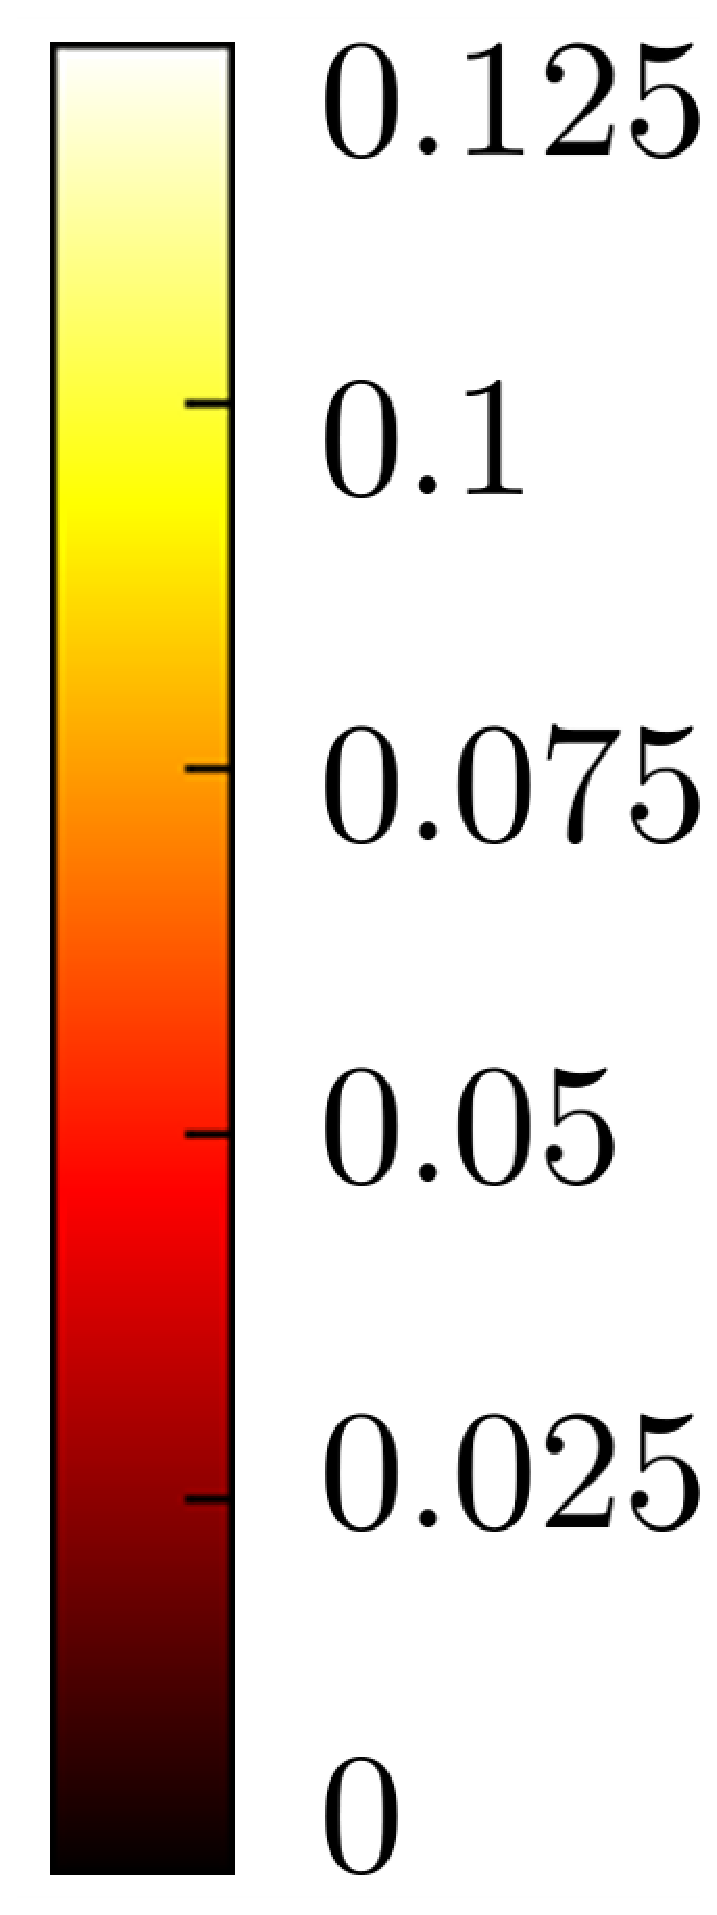
\includegraphics[width=\hsize]{./result_image/colorbar_hot}} % colorbar
		\end{minipage}
		
		\vspace{1mm}
		
		%       \begin{minipage}{0.125\hsize}
			%           \centerline{\small{Ground-truth}}
			% \end{minipage}
		% \begin{minipage}{0.125\hsize}
			% 	\centerline{\small{Observed noisy image}}
			% \end{minipage}
		% \begin{minipage}{0.125\hsize}
			% 	\centerline{\small{SSTV}}
			% \end{minipage}
		% \begin{minipage}{0.125\hsize}
			% 	\centerline{\small{HSSTV1}}
			% \end{minipage}
		% \begin{minipage}{0.125\hsize}
			% 	\centerline{\small{HSSTV2}}
			% \end{minipage}
		%       \begin{minipage}{0.125\hsize}
			% 	\centerline{\small{$\llHTV$}}
			% \end{minipage}
		\begin{minipage}{0.125\hsize}
			\centerline{\small{(a)}}
		\end{minipage}
		\begin{minipage}{0.125\hsize}
			\centerline{\small{(b)}}
		\end{minipage}
		\begin{minipage}{0.125\hsize}
			\centerline{\small{(c)}}
		\end{minipage}
		\begin{minipage}{0.125\hsize}
			\centerline{\small{(d)}}
		\end{minipage}
		\begin{minipage}{0.125\hsize}
			\centerline{\small{(e)}}
		\end{minipage}
		\begin{minipage}{0.125\hsize}
			\centerline{\small{(f)}}
		\end{minipage}
		\begin{minipage}{0.125\hsize}
			\centerline{\small{(g)}}
		\end{minipage}
		\begin{minipage}{0.050\hsize}
			\centerline{\hspace{\hsize}} % Space
		\end{minipage}
		
		%       \begin{minipage}{0.125\hsize}
			%           \centerline{\small{MPSNR [dB]}}
			% \end{minipage}
		% \begin{minipage}{0.125\hsize}
			% 	\centerline{\small{16.86 [dB]}} % noisy
			% \end{minipage}
		% \begin{minipage}{0.125\hsize}
			% 	\centerline{\small{39.32 [dB]}} % SSTV
			% \end{minipage}
		% \begin{minipage}{0.125\hsize}
			% 	\centerline{\small{38.98 [dB]}} % HSSTV1
			% \end{minipage}
		% \begin{minipage}{0.125\hsize}
			% 	\centerline{\small{38.92 [dB]}} % HSSTV2
			% \end{minipage}
		%       \begin{minipage}{0.125\hsize}
			% 	\centerline{\small{38.47 [dB]}} % l0l1HTV
			% \end{minipage}
		%       \begin{minipage}{0.050\hsize}
			%           \centerline{\hspace{\hsize}} % Space
			% \end{minipage}
		
		\vspace{2mm}
		
		\begin{minipage}{0.125\hsize}
			\centerline{\includegraphics[width=\hsize]{./result_image/Case1_PaviaU120/restored_image/b44_m1.5/image_SSST.eps}} % SSST image
		\end{minipage}
		\begin{minipage}{0.125\hsize}
			\centerline{\includegraphics[width=\hsize]{./result_image/Case1_PaviaU120/restored_image/b44_m1.5/image_LRTDTV.eps}} % LRTDTV image
		\end{minipage}
		\begin{minipage}{0.125\hsize}
			\centerline{\includegraphics[width=\hsize]{./result_image/Case1_PaviaU120/restored_image/b44_m1.5/image_FGSLR.eps}} % FGSLR image
		\end{minipage}
		\begin{minipage}{0.125\hsize}
			\centerline{\includegraphics[width=\hsize]{./result_image/Case1_PaviaU120/restored_image/b44_m1.5/image_TPTV.eps}} % TPTV image
		\end{minipage}
		\begin{minipage}{0.125\hsize}
			\centerline{\includegraphics[width=\hsize]{./result_image/Case1_PaviaU120/restored_image/b44_m1.5/image_QRNN3D.eps}} % QRNN3D image
		\end{minipage}
		\begin{minipage}{0.125\hsize}
			\centerline{\includegraphics[width=\hsize]{./result_image/Case1_PaviaU120/restored_image/b44_m1.5/image_FastHyMix.eps}} % FastHyMix image
		\end{minipage}
		\begin{minipage}{0.125\hsize}
			\centerline{\includegraphics[width=\hsize]{./result_image/Case1_PaviaU120/restored_image/b44_m1.5/image_S3TTV.eps}} % S3TTV image
		\end{minipage}
		\begin{minipage}{0.050\hsize}
			\centerline{\hspace{\hsize}} % Space
		\end{minipage}
		
		\vspace{1mm}
		
		\begin{minipage}{0.125\hsize}
			\centerline{\includegraphics[width=\hsize]{./result_image/Case1_PaviaU120/diff_image/b44_m1.5_hot/diff_image_SSST.eps}} % SSST diff image
		\end{minipage}
		\begin{minipage}{0.125\hsize}
			\centerline{\includegraphics[width=\hsize]{./result_image/Case1_PaviaU120/diff_image/b44_m1.5_hot/diff_image_LRTDTV.eps}} % LRTDTV diff image
		\end{minipage}
		\begin{minipage}{0.125\hsize}
			\centerline{\includegraphics[width=\hsize]{./result_image/Case1_PaviaU120/diff_image/b44_m1.5_hot/diff_image_FGSLR.eps}} % FGSLR diff image
		\end{minipage}
		\begin{minipage}{0.125\hsize}
			\centerline{\includegraphics[width=\hsize]{./result_image/Case1_PaviaU120/diff_image/b44_m1.5_hot/diff_image_TPTV.eps}} % TPTV diff image
		\end{minipage}
		\begin{minipage}{0.125\hsize}
			\centerline{\includegraphics[width=\hsize]{./result_image/Case1_PaviaU120/diff_image/b44_m1.5_hot/diff_image_QRNN3D.eps}} % QRNN3D diff image
		\end{minipage}
		\begin{minipage}{0.125\hsize}
			\centerline{\includegraphics[width=\hsize]{./result_image/Case1_PaviaU120/diff_image/b44_m1.5_hot/diff_image_FastHyMix.eps}} % FastHyMix diff image
		\end{minipage}
		\begin{minipage}{0.125\hsize}
			\centerline{\includegraphics[width=\hsize]{./result_image/Case1_PaviaU120/diff_image/b44_m1.5_hot/diff_image_S3TTV.eps}} % S3TTV diff image
		\end{minipage}
		\begin{minipage}{0.050\hsize}
			\centerline{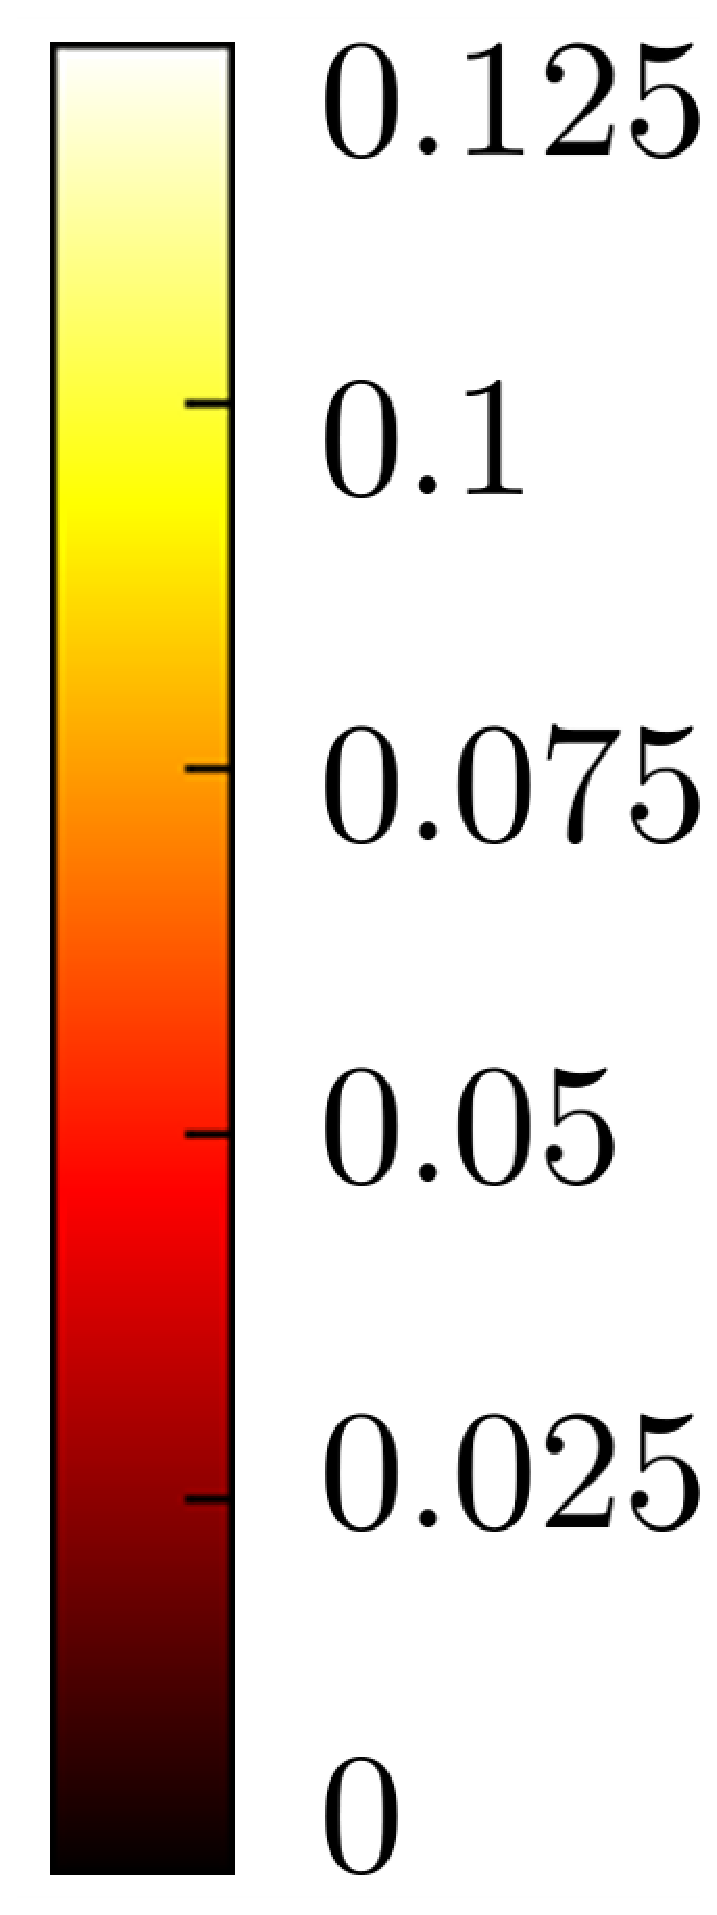
\includegraphics[width=\hsize]{./result_image/colorbar_hot}} % colorbar
		\end{minipage}
		
		\vspace{1mm}
		
		\begin{minipage}{0.125\hsize}
			\centerline{\small{(h)}}
		\end{minipage}
		\begin{minipage}{0.125\hsize}
			\centerline{\small{(i)}}
		\end{minipage}
		\begin{minipage}{0.125\hsize}
			\centerline{\small{(j)}}
		\end{minipage}
		\begin{minipage}{0.125\hsize}
			\centerline{\small{(k)}}
		\end{minipage}
		\begin{minipage}{0.125\hsize}
			\centerline{\small{(l)}}
		\end{minipage}
		\begin{minipage}{0.125\hsize}
			\centerline{\small{(m)}}
		\end{minipage}
		\begin{minipage}{0.125\hsize}
			\centerline{\small{(n)}}
		\end{minipage}
		\begin{minipage}{0.050\hsize}
			\centerline{\hspace{\hsize}} % Space
		\end{minipage}
		
		
		%       \begin{minipage}{0.125\hsize}
			%           \centerline{\hspace{\hsize}} % Space
			% \end{minipage}
		%       \begin{minipage}{0.125\hsize}
			%           \centerline{\small{\textbf{40.29} [dB]}} % TPTV
			% \end{minipage}
		% \begin{minipage}{0.125\hsize}
			%           \centerline{\small{29.81 [dB]}} % STV
			% \end{minipage}
		% \begin{minipage}{0.125\hsize}
			%           \centerline{\small{36.56 [dB]}} % SSST
			% \end{minipage}
		% \begin{minipage}{0.125\hsize}
			%           \centerline{\small{37.85 [dB]}} % LRTDTV
			% \end{minipage}
		% \begin{minipage}{0.125\hsize}
			%           \centerline{\small{\underline{39.83} [dB]}} % S3TTV
			% \end{minipage}
		%       \begin{minipage}{0.050\hsize}
			%           \centerline{\hspace{\hsize}} % Space
			% \end{minipage}
	\end{center}
	
	\vspace{-3mm}
	\caption{Denoising results for Pavia University with the 44th band in Case 1. Upper row images are the restored images by each method. Lower row images are the absolute difference between the original image and each restored image (the range of the only observed noisy image in $\IndexNoisy$ is $[0,1]$). (a) Ground-truth. (b) Observed noisy image. (c) SSTV. (d) HSSTV1. (e) HSSTV2. (f) $\llHTV$. (g) STV. (h) SSST. (i) LRTDTV. (j) FGSLR. (k) TPTV. (l) QRNN3D. (m) FastHyMix. (n) $\SSSTTV$ (ours).}
	\label{fig:result_image_Case1_PU}
\end{figure*}
To demonstrate the effectiveness of $\SSSTTV$, we conducted mixed noise removal experiments on HS image contaminated with simulated or real noise.
We compared $\SSSTTV$ with four types of methods; SSTV-based methods, i.e., SSTV~\cite{Aggarwal2016SSTV}, HSSTV~\cite{Takeyama2020HSSTV}, and $\llHTV$~\cite{Wang2021l0l1HTV}; STV-based methods, i.e., STV~\cite{Lefkimmiatis2015STV} and SSST~\cite{Kurihara2017SSST}; LR-based methods, i.e., LRTDTV~\cite{Wang2018LRTDTV}, FGSLR~\cite{Chen2022FGSLR}, and TPTV~\cite{Chen2023TPTV}; and DNN-based methods, i.e., QRNN3D~\cite{Wei2021QRNN3D} and FastHyMix~\cite{Zhuang2023FastHyMix}. 
Here, HSSTV with $\ell_{1}$-norm and $\ell_{1,2}$-norm are denoted by HSSTV1 and HSSTV2, respectively.
For a fair comparison, the regularization functions of the P-PDS applicable methods, i.e., SSTV, HSSTV1, HSSTV2, $\llHTV$, STV, and SSST, were replaced with the $\SSSTTV$ regularization function in Prob.~\eqref{prob:S3TTV_denoising}, and we solve each problem by P-PDS.
For LRTDTV, FGSLR, TPTV, QRNN3D, and FastHyMix, we used implementation codes published by the authors\footnote{The LRTDTV, FGSLR, TPTV, QRNN3D, and FastHyMix implementation codes are available at 
\\ https://github.com/zhaoxile/Hyperspectral-Image-Restoration-via-Total-Variation-Regularized-Low-rank-Tensor-Decomposition, \\https://chenyong1993.github.io/yongchen.github.io/, \\https://github.com/chuchulyf/ETPTV, \\https://github.com/Vandermode/QRNN3D?tab=readme-ov-file, \\and https://github.com/LinaZhuang/HSI-MixedNoiseRemoval-FastHyMix, respectively.}. For QRNN3D, we performed fine-tuning using Pavia Centre\footnote{\url{https://www.ehu/ccwintco/index/php/Hyperspectral_Remote_Sensing_Scenes}}to improve noise removal performance.
% For the parameters of existing methods, we used the values recommended in each reference.
% The experimental environment is MATLAB (R2023a) on a Windows 11 computer 
% %\begin{table*}[t]
%    \begin{center}
%        \caption{MPSNRs of the Simulated HS Image Denoising Results.}
%        \label{tab:MPSNR}
%            \scalebox{0.85}{
%        \begin{tabular}{cc ccccccccc}
%            \toprule
%                Image & Noise & SSTV~\cite{Aggarwal2016SSTV} & HSSTV1~\cite{Takeyama2020HSSTV} & HSSTV2~\cite{Takeyama2020HSSTV} & $\llHTV$~\cite{Wang2021l0l1HTV} & STV~\cite{Lefkimmiatis2015STV} & SSST~\cite{Kurihara2017SSST} & LRTDTV~\cite{Wang2018LRTDTV} & TPTV~\cite{Chen2023TPTV} & $\SSSTTV$ \\
%            \cmidrule(lr){1-11}
%            % \vspace{-0.5mm}
%                \multirow{6}{*}{Jasper Ridge} & Case 1 & 
%                39.32 & 38.98 & 38.92 & 38.47 & 29.81 & 36.56 & 37.85 & \textbf{40.29} & \underline{39.82}\\
%                & Case 2 & 
%                34.24 & 34.01 & 34.67 & 34.00 & 27.23 & 32.07 & 34.87 & \underline{35.79} & \textbf{36.00} \\
%                & Case 3 & 
%                39.07 & \underline{39.29} & 38.31 & 38.92 & 30.72 & 37.63 & 35.99 & 38.14 & \textbf{40.10} \\
%                & Case 4 & 
%                34.21 & 34.81 & 33.90 & 34.68 & 28.08 & 34.88 & 33.69 & \underline{35.51} & \textbf{35.72} \\
%                & Case 5 & 
%                39.30 & 39.06 & 38.55 & 38.35 & 29.54 & 35.67 & 36.05 & \underline{39.24} & \textbf{39.65} \\
%                & Case 6 & 
%                34.59 & 34.22 & 34.99 & 34.15 & 26.95 & 30.95 & 33.64 & \underline{35.23} & \textbf{35.89} \\
%
%            \cmidrule(lr){1-11}
%            
%            \multirow{6}{*}{Pavia University} & Case 1 & 
%            	38.43 & 38.34 & 38.23 & 37.88 & 29.84 & 35.16 & 35.08 & \underline{38.74} & \textbf{39.24} \\
%                & Case 2 & 
%                32.87 & 33.38 & 33.07 & 32.67 & 27.49 & 31.63 & 32.53 & \textbf{34.12} & \underline{33.94}  \\
%                & Case 3 & 
%                39.34 & \underline{39.43} & 38.43 & 39.04 & 30.74 & 36.52 & 32.34 & 38.14 & \textbf{39.80}  \\
%                & Case 4 & 
%                34.26 &\underline{34.88} & 33.82 & 34.75 & 28.33 & 34.69 & 30.82 & 34.03 & \textbf{35.17} \\
%                & Case 5 & 
%                \underline{38.56} & 38.48 & 38.22 & 37.73 & 29.62 & 34.25 & 32.44 & 38.29 & \textbf{38.78} \\
%                & Case 6 & 
%                32.88 & 33.42 & 33.19 & 32.52 & 27.24 & 30.50 & 30.89 & \underline{33.67} & \textbf{33.88} \\
%	            
%            \bottomrule
%        \end{tabular}
%        		}
%    \end{center}
%    % \vspace{-3mm}
%\end{table*}


\begin{table*}[t]
	\begin{center}
		\caption{MPSNRs of the Simulated HS Image Denoising Results.}
		\label{tab:MPSNR}
		\scalebox{0.75}{
			\begin{tabular}{cc ccccccccccc}
				\toprule
				Image & Noise & SSTV~\cite{Aggarwal2016SSTV} & HSSTV1~\cite{Takeyama2020HSSTV} & HSSTV2~\cite{Takeyama2020HSSTV} & $\llHTV$~\cite{Wang2021l0l1HTV} & STV~\cite{Lefkimmiatis2015STV} & SSST~\cite{Kurihara2017SSST} & LRTDTV~\cite{Wang2018LRTDTV} & FGSLR~\cite{Chen2022FGSLR} & TPTV~\cite{Chen2023TPTV} & FastHyMix~\cite{Zhuang2023FastHyMix} & $\SSSTTV$ \\
				\cmidrule(lr){1-13}
				% \vspace{-0.5mm}
				\multirow{8}{*}{Jasper Ridge} 
				& Case 1 &
				36.16 & \underline{36.25} & 35.66 & 35.40 & 28.15 & 35.03 & 35.08 & 33.68 & 34.25 & \textbf{38.77} & 35.43 \\
				& Case 2 & 
				\underline{39.32} & 38.98 & 38.92 & 38.47 & 29.81 & 36.56 & 37.85 & 35.65 & 39.01 & 27.86 & \textbf{39.82} \\
				& Case 3 & 
				34.24 & 34.01 & 34.67 & 34.00 & 27.23 & 32.07 & \underline{34.87} & 33.44 & 33.68 & 25.53 & \textbf{36.00} \\
				& Case 4 &
				42.50 & 41.45 & \underline{44.46} & 42.95 & 39.09 & 41.31 & 37.07 & 41.65 & \textbf{51.34} & 34.93 & 43.95 \\
				& Case 5 & 
				39.03 & \underline{39.26} & 38.33 & 38.88 & 30.72 & 37.63 & 36.00 & 35.62 & 37.92 & 35.21 & \textbf{39.90} \\
				& Case 6 & 
				34.19 & 34.79 & 33.91 & 34.52 & 28.08 & \underline{34.88} & 33.70 & 33.43 & 33.44 & 34.30 & \textbf{35.41} \\
				& Case 7 & 
				\underline{39.30} & 39.06 & 38.55 & 38.35 & 29.54 & 35.67 & 36.09 & 35.46 & 37.91 & 37.29 & \textbf{39.65} \\
				& Case 8 & 
				34.59 & 34.22 & \underline{34.99} & 34.15 & 26.95 & 30.95 & 33.64 & 33.23 & 33.08 & 23.19 & \textbf{35.89} \\
				
				\cmidrule(lr){1-13}
				
				\multirow{8}{*}{Pavia University}
				& Case 1 &
				35.64 & \underline{36.05} & 34.98 & 35.08 & 28.33 & 34.85 & 32.67 & 32.52 & 31.41 & \textbf{37.53} & 35.37 \\
				& Case 2 & 
				38.43 & 38.34 & 38.23 & 37.88 & 29.84 & 35.16 & 35.08 & 35.33 & 36.80 & \underline{38.91} & \textbf{39.24} \\
				& Case 3 & 
				32.87 & 33.38 & 33.07 & 32.67 & 27.49 & 31.63 & 32.53 & 31.88 & 31.04 & \textbf{35.91} & \underline{33.94} \\
				& Case 4 &
				41.01 & 40.50 & \underline{43.96} & 41.81 & 39.28 & 40.43 & 32.22 & 40.07 & \textbf{48.14} & 34.24 & 42.62 \\
				& Case 5 & 
				39.32 & \underline{39.42} & 38.44 & 39.06 & 30.74 & 36.52 & 32.34 & 35.41 & 35.75 & 34.70 & \textbf{39.78} \\
				& Case 6 & 
				34.24 & \underline{34.87} & 33.82 & 34.65 & 28.33 & 34.69 & 30.87 & 31.84 & 31.56 & 33.57 & \textbf{35.17} \\
				& Case 7 & 
				\underline{38.56} & 38.48 & 38.22 & 37.73 & 29.62 & 34.25 & 32.43 & 35.12 & 35.72 & 32.02 & \textbf{38.78} \\
				& Case 8 & 
				32.88 & \underline{33.42} & 33.19 & 32.52 & 27.24 & 30.50 & 30.88 & 31.65 & 31.06 & 31.77 & \textbf{33.88} \\
				
				\cmidrule(lr){1-13}
				
				\multirow{8}{*}{Beltsville}
				& Case 1 &
				35.20 & \underline{35.90} & 34.87 & 34.70 & 29.11 & 35.86 & 34.23 & 34.68 & 32.24 & \textbf{39.36} & 35.33 \\
				& Case 2 & 
				37.87 & 38.18 & 37.62 & 37.32 & 30.83 & 36.81 & \underline{38.71} & 36.73 & 37.82 & 37.86 & \textbf{39.40} \\
				& Case 3 & 
				32.95 & 33.94 & 32.93 & 32.76 & 28.39 & 32.39 & 34.18 & \underline{34.45} & 31.76 & \textbf{36.12} & 34.23 \\
				& Case 4 &
				41.16 & 40.84 & 41.37 & 41.45 & 37.96 & 40.21 & 38.69 & \underline{42.90} & \textbf{52.72} & 36.22 & 40.72 \\
				& Case 5 & 
				38.43 & \underline{38.73} & 37.99 & 38.11 & 30.73 & 37.04 & 33.47 & 36.64 & 36.68 & 35.11 & \textbf{39.65} \\
				& Case 6 & 
				33.91 & 34.64 & 33.72 & 34.20 & 28.62 & \underline{34.81} & 30.60 & 34.25 & 32.84 & 34.12 & \textbf{35.29} \\
				& Case 7 & 
				38.00 & \underline{38.21} & 37.62 & 37.21 & 30.05 & 35.43 & 32.97 & 36.45 & 36.99 & 37.18 & \textbf{38.85} \\
				& Case 8 & 
				33.14 & 33.98 & 33.25 & 32.72 & 27.84 & 30.97 & 30.59 & \underline{34.05} & 32.26 & 33.33 & \textbf{34.43} \\
				
				\bottomrule
			\end{tabular}
		}
	\end{center}
	% \vspace{-3mm}
\end{table*}
% \begin{table*}[t]
    \begin{center}
        \caption{MSSIMs of the Simulated HS Image Denoising Results.}
        \label{tab:MSSIM}
        		\scalebox{0.75}{
        \begin{tabular}{cc ccccccccccc}
            \toprule
                Image & Noise & SSTV~\cite{Aggarwal2016SSTV} & HSSTV1~\cite{Takeyama2020HSSTV} & HSSTV2~\cite{Takeyama2020HSSTV} & $\llHTV$~\cite{Wang2021l0l1HTV} & STV~\cite{Lefkimmiatis2015STV} & SSST~\cite{Kurihara2017SSST} & LRTDTV~\cite{Wang2018LRTDTV} & FGSLR~\cite{Chen2022FGSLR} & TPTV~\cite{Chen2023TPTV} & FastHyMix~\cite{Zhuang2023FastHyMix} & $\SSSTTV$ \\
            \cmidrule(lr){1-13}
            % \vspace{-0.5mm}
				\multirow{8}{*}{Jasper Ridge}
				& Case 1 & 
				0.9218 & \underline{0.9367} & 0.9170 & 0.9013 & 0.7495 & 0.9318 & 0.9147 & 0.9175 & 0.8703 & \textbf{0.9659} & 0.9070 \\
				& Case 2 & 
                0.9588 & \textbf{0.9632} & 0.9552 & 0.9468 & 0.8227 & 0.9486 & 0.9542 & 0.9450 & 0.9504 & 0.8648 & \underline{0.9601} \\
                & Case 3 & 
                0.9026 & 0.9071 & 0.9082 & 0.8897 & 0.7165 & 0.8736 & 0.9122 & \underline{0.9144} & 0.8613 & 0.7726 & \textbf{0.9201} \\
                & Case 4 & 
                0.9782 & 0.9759 & 0.9774 & 0.9782 & 0.9739 & 0.9780 & 0.9572 & \underline{0.9830} & \textbf{0.9889} & 0.9090 & 0.9788 \\
                & Case 5 & 
                0.9539 & \textbf{0.9613} & 0.9481 & 0.9490 & 0.8428 & 0.9586 & 0.9319 & 0.9434 & 0.9363 & 0.9037 & \underline{0.9608} \\
                & Case 6 & 
                0.8808 & 0.9054 & 0.8775 & 0.8832 & 0.7446 & \textbf{0.9296} & 0.8794 & \underline{0.9108} & 0.8519 & 0.8888 & 0.9077 \\
                & Case 7 & 
                0.9585 & \textbf{0.9634} & 0.9518 & 0.9449 & 0.8144 & 0.9390 & 0.9328 & 0.9421 & 0.9416 & 0.9503 & \underline{0.9592} \\
                & Case 8 & 
                0.9071 & 0.9108 & \underline{0.9114} & 0.8895 & 0.7061 & 0.8439 & 0.8814 & 0.9086 & 0.8471 & 0.5912 & \textbf{0.9191} \\

            \cmidrule(lr){1-13}
            
            	\multirow{8}{*}{Pavia University}
            	& Case 1 &
            	0.9207 & \underline{0.9347} & 0.9067 & 0.9088 & 0.7170 & 0.9231 & 0.8600 & 0.9013 & 0.8074 & \textbf{0.9533} & 0.9119 \\
            	& Case 2 & 
            	0.9559 & \underline{0.9585} & 0.9478 & 0.9486 & 0.7889 & 0.9307 & 0.9166 & 0.9412 & 0.9307 & \textbf{0.9698} & 0.9582 \\
                & Case 3 & 
                0.8731 & 0.8882 & 0.8731 & 0.8672 & 0.6754 & 0.8533 & 0.8573 & 0.8829 & 0.8011 & \textbf{0.9445} & \underline{0.8928} \\
                & Case 4 & 
                0.9726 & 0.9716 & 0.9753 & 0.9730 & 0.9723 & 0.9727 & 0.9055 & \textbf{0.9793} & 0.9750 & 0.9310 & \underline{0.9754} \\
                & Case 5 & 
                0.9622 & \textbf{0.9657} & 0.9514 & 0.9584 & 0.8191 & 0.9435 & 0.8789 & 0.9421 & 0.9162 & 0.9163 & \underline{0.9625} \\
                & Case 6 & 
                0.8933 & \underline{0.9133} & 0.8830 & 0.8998 & 0.7180 & \textbf{0.9213} & 0.8148 & 0.8955 & 0.8166 & 0.8955 & 0.9089 \\
                & Case 7 & 
                \underline{0.9573} & \textbf{0.9598} & 0.9482 & 0.9473 & 0.7812 & 0.9160 & 0.8776 & 0.9390 & 0.9207 & 0.9122 & 0.9550 \\
                & Case 8 & 
                0.8736 & \underline{0.8892} & 0.8752 & 0.8640 & 0.6639 & 0.8152 & 0.8139 & 0.8790 & 0.8059 & 0.8712 & \textbf{0.8915} \\
                
            \cmidrule(lr){1-13}
            
	            \multirow{8}{*}{Beltsville}
	            & Case 1 & 
	            0.9099 & 0.9290 & 0.9035 & 0.8978 & 0.7282 & \underline{0.9327} & 0.8776 & 0.9134 & 0.8137 & \textbf{0.9642} & 0.9052 \\
	            & Case 2 &
	            0.9497 & 0.9550 & 0.9458 & 0.9425 & 0.8012 & 0.9410 & 0.9508 & 0.9482 & 0.9421 & \textbf{0.9663} & \underline{0.9605} \\
	            & Case 3 & 
	            0.8710 & 0.8931 & 0.8694 & 0.8696 & 0.6911 & 0.8641 & 0.8784 & \underline{0.9094} & 0.8033 & \textbf{0.9458} & 0.8974 \\
	            & Case 4 & 
	            0.9719 & 0.9715 & 0.9716 & 0.9716 & 0.9564 & 0.9709 & 0.9568 & \textbf{0.9829} & \underline{0.9806} & 0.9413 & 0.9709 \\
	            & Case 5 & 
	            0.9524 & \underline{0.9590} & 0.9470 & 0.9490 & 0.8003 & 0.9459 & 0.8899 & 0.9483 & 0.9293 & 0.9136 & \textbf{0.9634} \\
	            & Case 6 & 
	            0.8776 & 0.9030 & 0.8724 & 0.8848 & 0.7071 & \textbf{0.9187} & 0.7916 & \underline{0.9097} & 0.8393 & 0.8932 & 0.9079 \\
	            & Case 7 & 
	            0.9512 & 0.9566 & 0.9456 & 0.9417 & 0.7740 & 0.9249 & 0.8879 & 0.9461 & 0.9294 & \underline{0.9539} & \textbf{0.9578} \\
	            & Case 8 & 
	            0.8753 & 0.8956 & 0.8761 & 0.8683 & 0.6637 & 0.8270 & 0.7906 & \textbf{0.9057} & 0.8564 & 0.8681 & \underline{0.9006} \\
            \bottomrule
        \end{tabular}
        		}
    \end{center}
    % \vspace{-3mm}
\end{table*}

\subsection{Simulated HS Image Experiments}
%\begin{figure*}[t]
	\begin{center}
		\begin{minipage}{0.125\hsize}
			\centerline{\includegraphics[width=\hsize]{./result_image/Case1_PaviaU120/restored_image/b44_m1.5/image_clean.eps}} % Ground-truth image
		\end{minipage}
		\begin{minipage}{0.125\hsize}
			\centerline{\includegraphics[width=\hsize]{./result_image/Case1_PaviaU120/restored_image/b44_m1.5/image_noisy.eps}} % noisy image
		\end{minipage}
		\begin{minipage}{0.125\hsize}
			\centerline{\includegraphics[width=\hsize]{./result_image/Case1_PaviaU120/restored_image/b44_m1.5/image_SSTV.eps}} % SSTV image
		\end{minipage}
		\begin{minipage}{0.125\hsize}
			\centerline{\includegraphics[width=\hsize]{./result_image/Case1_PaviaU120/restored_image/b44_m1.5/image_HSSTV_L1.eps}} % HSSTV L1 image
		\end{minipage}
		\begin{minipage}{0.125\hsize}
			\centerline{\includegraphics[width=\hsize]{./result_image/Case1_PaviaU120/restored_image/b44_m1.5/image_HSSTV_L12.eps}} % HSSTV L12 image
		\end{minipage}
		\begin{minipage}{0.125\hsize}
			\centerline{\includegraphics[width=\hsize]{./result_image/Case1_PaviaU120/restored_image/b44_m1.5/image_l0l1HTV.eps}} % l0l1HTV image
		\end{minipage}
		\begin{minipage}{0.125\hsize}
			\centerline{\includegraphics[width=\hsize]{./result_image/Case1_PaviaU120/restored_image/b44_m1.5/image_STV.eps}} % STV image
		\end{minipage}
		\begin{minipage}{0.050\hsize}
			\centerline{\hspace{\hsize}} % Space
		\end{minipage}
		
		\vspace{1mm}
		
		\begin{minipage}{0.125\hsize}
			\centerline{\hspace{\hsize}} % Space
		\end{minipage}
		\begin{minipage}{0.125\hsize}
			\centerline{\includegraphics[width=\hsize]{./result_image/Case1_PaviaU120/diff_image/b44_m1.5_hot/diff_image_noisy.eps}} % noisy diff image
		\end{minipage}
		\begin{minipage}{0.125\hsize}
			\centerline{\includegraphics[width=\hsize]{./result_image/Case1_PaviaU120/diff_image/b44_m1.5_hot/diff_image_SSTV.eps}} % SSTV diff image
		\end{minipage}
		\begin{minipage}{0.125\hsize}
			\centerline{\includegraphics[width=\hsize]{./result_image/Case1_PaviaU120/diff_image/b44_m1.5_hot/diff_image_HSSTV_L1.eps}} % HSSTV L1 diff image
		\end{minipage}
		\begin{minipage}{0.125\hsize}
			\centerline{\includegraphics[width=\hsize]{./result_image/Case1_PaviaU120/diff_image/b44_m1.5_hot/diff_image_HSSTV_L12.eps}} % HSSTV L12 diff image
		\end{minipage}
		\begin{minipage}{0.125\hsize}
			\centerline{\includegraphics[width=\hsize]{./result_image/Case1_PaviaU120/diff_image/b44_m1.5_hot/diff_image_l0l1HTV.eps}} % l0l1HTV diff image
		\end{minipage}
		\begin{minipage}{0.125\hsize}
			\centerline{\includegraphics[width=\hsize]{./result_image/Case1_PaviaU120/diff_image/b44_m1.5_hot/diff_image_STV.eps}} % STV diff image
		\end{minipage}
		\begin{minipage}{0.050\hsize}
			\centerline{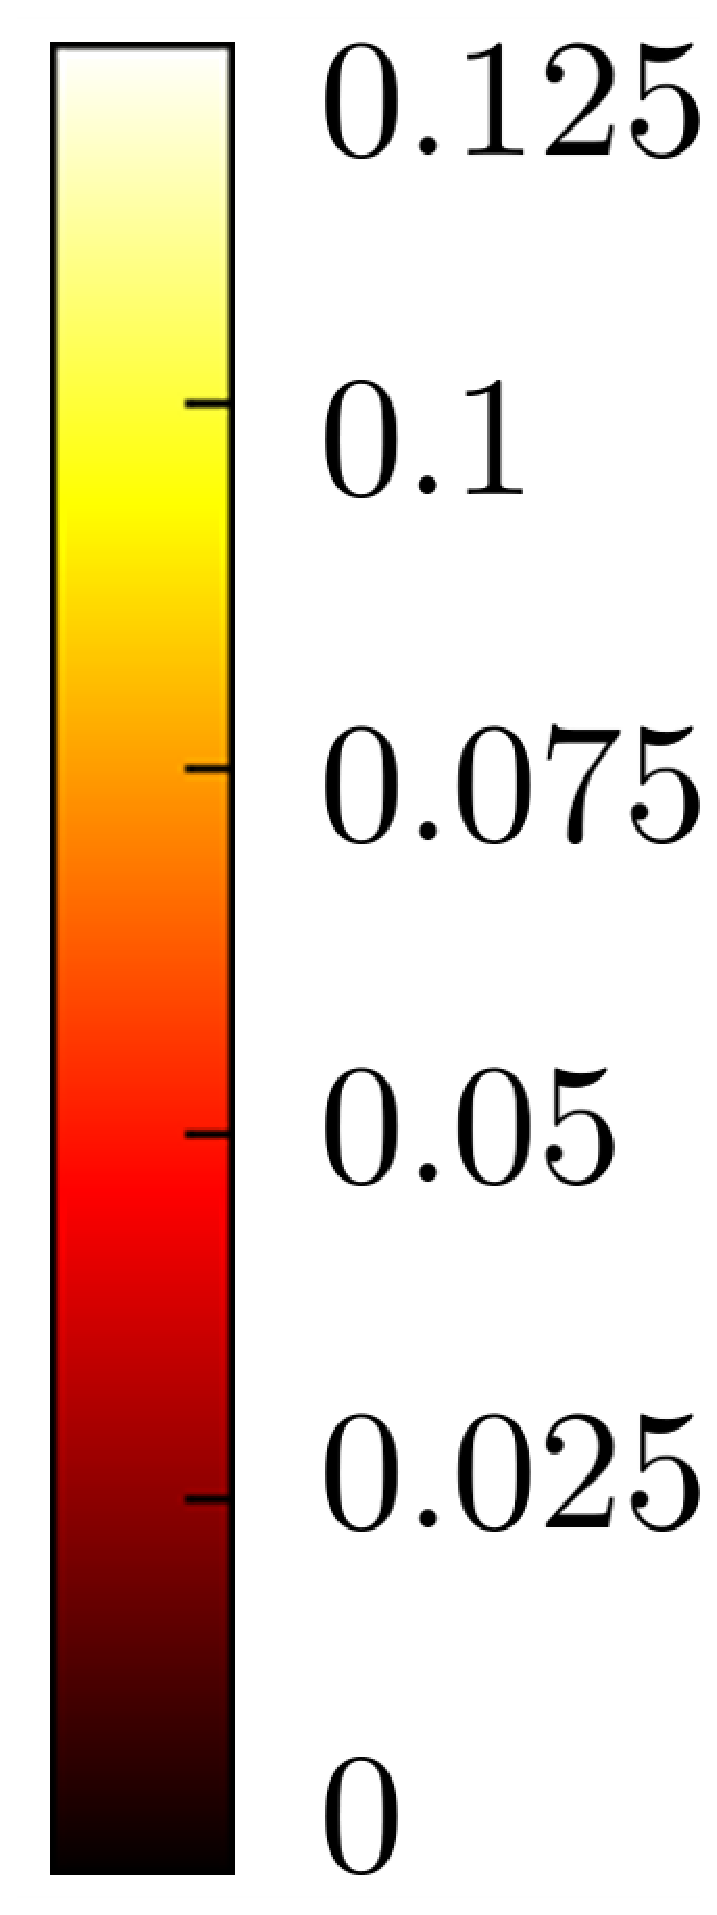
\includegraphics[width=\hsize]{./result_image/colorbar_hot}} % colorbar
		\end{minipage}
		
		\vspace{1mm}
		
		%       \begin{minipage}{0.125\hsize}
			%           \centerline{\small{Ground-truth}}
			% \end{minipage}
		% \begin{minipage}{0.125\hsize}
			% 	\centerline{\small{Observed noisy image}}
			% \end{minipage}
		% \begin{minipage}{0.125\hsize}
			% 	\centerline{\small{SSTV}}
			% \end{minipage}
		% \begin{minipage}{0.125\hsize}
			% 	\centerline{\small{HSSTV1}}
			% \end{minipage}
		% \begin{minipage}{0.125\hsize}
			% 	\centerline{\small{HSSTV2}}
			% \end{minipage}
		%       \begin{minipage}{0.125\hsize}
			% 	\centerline{\small{$\llHTV$}}
			% \end{minipage}
		\begin{minipage}{0.125\hsize}
			\centerline{\small{(a)}}
		\end{minipage}
		\begin{minipage}{0.125\hsize}
			\centerline{\small{(b)}}
		\end{minipage}
		\begin{minipage}{0.125\hsize}
			\centerline{\small{(c)}}
		\end{minipage}
		\begin{minipage}{0.125\hsize}
			\centerline{\small{(d)}}
		\end{minipage}
		\begin{minipage}{0.125\hsize}
			\centerline{\small{(e)}}
		\end{minipage}
		\begin{minipage}{0.125\hsize}
			\centerline{\small{(f)}}
		\end{minipage}
		\begin{minipage}{0.125\hsize}
			\centerline{\small{(g)}}
		\end{minipage}
		\begin{minipage}{0.050\hsize}
			\centerline{\hspace{\hsize}} % Space
		\end{minipage}
		
		%       \begin{minipage}{0.125\hsize}
			%           \centerline{\small{MPSNR [dB]}}
			% \end{minipage}
		% \begin{minipage}{0.125\hsize}
			% 	\centerline{\small{16.86 [dB]}} % noisy
			% \end{minipage}
		% \begin{minipage}{0.125\hsize}
			% 	\centerline{\small{39.32 [dB]}} % SSTV
			% \end{minipage}
		% \begin{minipage}{0.125\hsize}
			% 	\centerline{\small{38.98 [dB]}} % HSSTV1
			% \end{minipage}
		% \begin{minipage}{0.125\hsize}
			% 	\centerline{\small{38.92 [dB]}} % HSSTV2
			% \end{minipage}
		%       \begin{minipage}{0.125\hsize}
			% 	\centerline{\small{38.47 [dB]}} % l0l1HTV
			% \end{minipage}
		%       \begin{minipage}{0.050\hsize}
			%           \centerline{\hspace{\hsize}} % Space
			% \end{minipage}
		
		\vspace{2mm}
		
		\begin{minipage}{0.125\hsize}
			\centerline{\includegraphics[width=\hsize]{./result_image/Case1_PaviaU120/restored_image/b44_m1.5/image_SSST.eps}} % SSST image
		\end{minipage}
		\begin{minipage}{0.125\hsize}
			\centerline{\includegraphics[width=\hsize]{./result_image/Case1_PaviaU120/restored_image/b44_m1.5/image_LRTDTV.eps}} % LRTDTV image
		\end{minipage}
		\begin{minipage}{0.125\hsize}
			\centerline{\includegraphics[width=\hsize]{./result_image/Case1_PaviaU120/restored_image/b44_m1.5/image_FGSLR.eps}} % FGSLR image
		\end{minipage}
		\begin{minipage}{0.125\hsize}
			\centerline{\includegraphics[width=\hsize]{./result_image/Case1_PaviaU120/restored_image/b44_m1.5/image_TPTV.eps}} % TPTV image
		\end{minipage}
		\begin{minipage}{0.125\hsize}
			\centerline{\includegraphics[width=\hsize]{./result_image/Case1_PaviaU120/restored_image/b44_m1.5/image_QRNN3D.eps}} % QRNN3D image
		\end{minipage}
		\begin{minipage}{0.125\hsize}
			\centerline{\includegraphics[width=\hsize]{./result_image/Case1_PaviaU120/restored_image/b44_m1.5/image_FastHyMix.eps}} % FastHyMix image
		\end{minipage}
		\begin{minipage}{0.125\hsize}
			\centerline{\includegraphics[width=\hsize]{./result_image/Case1_PaviaU120/restored_image/b44_m1.5/image_S3TTV.eps}} % S3TTV image
		\end{minipage}
		\begin{minipage}{0.050\hsize}
			\centerline{\hspace{\hsize}} % Space
		\end{minipage}
		
		\vspace{1mm}
		
		\begin{minipage}{0.125\hsize}
			\centerline{\includegraphics[width=\hsize]{./result_image/Case1_PaviaU120/diff_image/b44_m1.5_hot/diff_image_SSST.eps}} % SSST diff image
		\end{minipage}
		\begin{minipage}{0.125\hsize}
			\centerline{\includegraphics[width=\hsize]{./result_image/Case1_PaviaU120/diff_image/b44_m1.5_hot/diff_image_LRTDTV.eps}} % LRTDTV diff image
		\end{minipage}
		\begin{minipage}{0.125\hsize}
			\centerline{\includegraphics[width=\hsize]{./result_image/Case1_PaviaU120/diff_image/b44_m1.5_hot/diff_image_FGSLR.eps}} % FGSLR diff image
		\end{minipage}
		\begin{minipage}{0.125\hsize}
			\centerline{\includegraphics[width=\hsize]{./result_image/Case1_PaviaU120/diff_image/b44_m1.5_hot/diff_image_TPTV.eps}} % TPTV diff image
		\end{minipage}
		\begin{minipage}{0.125\hsize}
			\centerline{\includegraphics[width=\hsize]{./result_image/Case1_PaviaU120/diff_image/b44_m1.5_hot/diff_image_QRNN3D.eps}} % QRNN3D diff image
		\end{minipage}
		\begin{minipage}{0.125\hsize}
			\centerline{\includegraphics[width=\hsize]{./result_image/Case1_PaviaU120/diff_image/b44_m1.5_hot/diff_image_FastHyMix.eps}} % FastHyMix diff image
		\end{minipage}
		\begin{minipage}{0.125\hsize}
			\centerline{\includegraphics[width=\hsize]{./result_image/Case1_PaviaU120/diff_image/b44_m1.5_hot/diff_image_S3TTV.eps}} % S3TTV diff image
		\end{minipage}
		\begin{minipage}{0.050\hsize}
			\centerline{\includegraphics[width=\hsize]{./result_image/colorbar_hot}} % colorbar
		\end{minipage}
		
		\vspace{1mm}
		
		\begin{minipage}{0.125\hsize}
			\centerline{\small{(h)}}
		\end{minipage}
		\begin{minipage}{0.125\hsize}
			\centerline{\small{(i)}}
		\end{minipage}
		\begin{minipage}{0.125\hsize}
			\centerline{\small{(j)}}
		\end{minipage}
		\begin{minipage}{0.125\hsize}
			\centerline{\small{(k)}}
		\end{minipage}
		\begin{minipage}{0.125\hsize}
			\centerline{\small{(l)}}
		\end{minipage}
		\begin{minipage}{0.125\hsize}
			\centerline{\small{(m)}}
		\end{minipage}
		\begin{minipage}{0.125\hsize}
			\centerline{\small{(n)}}
		\end{minipage}
		\begin{minipage}{0.050\hsize}
			\centerline{\hspace{\hsize}} % Space
		\end{minipage}
		
		
		%       \begin{minipage}{0.125\hsize}
			%           \centerline{\hspace{\hsize}} % Space
			% \end{minipage}
		%       \begin{minipage}{0.125\hsize}
			%           \centerline{\small{\textbf{40.29} [dB]}} % TPTV
			% \end{minipage}
		% \begin{minipage}{0.125\hsize}
			%           \centerline{\small{29.81 [dB]}} % STV
			% \end{minipage}
		% \begin{minipage}{0.125\hsize}
			%           \centerline{\small{36.56 [dB]}} % SSST
			% \end{minipage}
		% \begin{minipage}{0.125\hsize}
			%           \centerline{\small{37.85 [dB]}} % LRTDTV
			% \end{minipage}
		% \begin{minipage}{0.125\hsize}
			%           \centerline{\small{\underline{39.83} [dB]}} % S3TTV
			% \end{minipage}
		%       \begin{minipage}{0.050\hsize}
			%           \centerline{\hspace{\hsize}} % Space
			% \end{minipage}
	\end{center}
	
	\vspace{-3mm}
	\caption{Denoising results for Pavia University with the 44th band in Case 1. Upper row images are the restored images by each method. Lower row images are the absolute difference between the original image and each restored image (the range of the only observed noisy image in $\IndexNoisy$ is $[0,1]$). (a) Ground-truth. (b) Observed noisy image. (c) SSTV. (d) HSSTV1. (e) HSSTV2. (f) $\llHTV$. (g) STV. (h) SSST. (i) LRTDTV. (j) FGSLR. (k) TPTV. (l) QRNN3D. (m) FastHyMix. (n) $\SSSTTV$ (ours).}
	\label{fig:result_image_Case1_PU}
\end{figure*}
\begin{figure*}[t]
	\begin{center}
		\begin{minipage}{0.125\hsize}
			\centerline{\includegraphics[width=\hsize]{./result_image/Case3_JasperRidge/restored_image/b91_m1/image_clean.eps}} % Ground-truth image
		\end{minipage}
		\begin{minipage}{0.125\hsize}
			\centerline{\includegraphics[width=\hsize]{./result_image/Case3_JasperRidge/restored_image/b91_m1/image_noisy.eps}} % noisy image
		\end{minipage}
		\begin{minipage}{0.125\hsize}
			\centerline{\includegraphics[width=\hsize]{./result_image/Case3_JasperRidge/restored_image/b91_m1/image_SSTV.eps}} % SSTV image
		\end{minipage}
		\begin{minipage}{0.125\hsize}
			\centerline{\includegraphics[width=\hsize]{./result_image/Case3_JasperRidge/restored_image/b91_m1/image_HSSTV_L1.eps}} % HSSTV L1 image
		\end{minipage}
		\begin{minipage}{0.125\hsize}
			\centerline{\includegraphics[width=\hsize]{./result_image/Case3_JasperRidge/restored_image/b91_m1/image_HSSTV_L12.eps}} % HSSTV L12 image
		\end{minipage}
		\begin{minipage}{0.125\hsize}
			\centerline{\includegraphics[width=\hsize]{./result_image/Case3_JasperRidge/restored_image/b91_m1/image_l0l1HTV.eps}} % l0l1HTV image
		\end{minipage}
		\begin{minipage}{0.125\hsize}
			\centerline{\includegraphics[width=\hsize]{./result_image/Case3_JasperRidge/restored_image/b91_m1/image_STV.eps}} % STV image
		\end{minipage}
		\begin{minipage}{0.050\hsize}
			\centerline{\hspace{\hsize}} % Space
		\end{minipage}
		
		\vspace{1mm}
		
		\begin{minipage}{0.125\hsize}
			\centerline{\hspace{\hsize}} % Space
		\end{minipage}
		\begin{minipage}{0.125\hsize}
			\centerline{\includegraphics[width=\hsize]{./result_image/Case3_JasperRidge/diff_image/b91_m1_hot/diff_image_noisy.eps}} % noisy diff image
		\end{minipage}
		\begin{minipage}{0.125\hsize}
			\centerline{\includegraphics[width=\hsize]{./result_image/Case3_JasperRidge/diff_image/b91_m1_hot/diff_image_SSTV.eps}} % SSTV diff image
		\end{minipage}
		\begin{minipage}{0.125\hsize}
			\centerline{\includegraphics[width=\hsize]{./result_image/Case3_JasperRidge/diff_image/b91_m1_hot/diff_image_HSSTV_L1.eps}} % HSSTV L1 diff image
		\end{minipage}
		\begin{minipage}{0.125\hsize}
			\centerline{\includegraphics[width=\hsize]{./result_image/Case3_JasperRidge/diff_image/b91_m1_hot/diff_image_HSSTV_L12.eps}} % HSSTV L12 diff image
		\end{minipage}
		\begin{minipage}{0.125\hsize}
			\centerline{\includegraphics[width=\hsize]{./result_image/Case3_JasperRidge/diff_image/b91_m1_hot/diff_image_l0l1HTV.eps}} % l0l1HTV diff image
		\end{minipage}
		\begin{minipage}{0.125\hsize}
			\centerline{\includegraphics[width=\hsize]{./result_image/Case3_JasperRidge/diff_image/b91_m1_hot/diff_image_STV.eps}} % STV diff image
		\end{minipage}
		\begin{minipage}{0.050\hsize}
			\centerline{\includegraphics[width=\hsize]{./result_image/colorbar_hot}} % colorbar
		\end{minipage}
		
		\vspace{1mm}
		
		%       \begin{minipage}{0.125\hsize}
			%           \centerline{\small{Ground-truth}}
			% \end{minipage}
		% \begin{minipage}{0.125\hsize}
			% 	\centerline{\small{Observed noisy image}}
			% \end{minipage}
		% \begin{minipage}{0.125\hsize}
			% 	\centerline{\small{SSTV}}
			% \end{minipage}
		% \begin{minipage}{0.125\hsize}
			% 	\centerline{\small{HSSTV1}}
			% \end{minipage}
		% \begin{minipage}{0.125\hsize}
			% 	\centerline{\small{HSSTV2}}
			% \end{minipage}
		%       \begin{minipage}{0.125\hsize}
			% 	\centerline{\small{$\llHTV$}}
			% \end{minipage}
		\begin{minipage}{0.125\hsize}
			\centerline{\small{(a)}}
		\end{minipage}
		\begin{minipage}{0.125\hsize}
			\centerline{\small{(b)}}
		\end{minipage}
		\begin{minipage}{0.125\hsize}
			\centerline{\small{(c)}}
		\end{minipage}
		\begin{minipage}{0.125\hsize}
			\centerline{\small{(d)}}
		\end{minipage}
		\begin{minipage}{0.125\hsize}
			\centerline{\small{(e)}}
		\end{minipage}
		\begin{minipage}{0.125\hsize}
			\centerline{\small{(f)}}
		\end{minipage}
		\begin{minipage}{0.125\hsize}
			\centerline{\small{(g)}}
		\end{minipage}
		\begin{minipage}{0.050\hsize}
			\centerline{\hspace{\hsize}} % Space
		\end{minipage}
		
		%       \begin{minipage}{0.125\hsize}
			%           \centerline{\small{MPSNR [dB]}}
			% \end{minipage}
		% \begin{minipage}{0.125\hsize}
			% 	\centerline{\small{16.86 [dB]}} % noisy
			% \end{minipage}
		% \begin{minipage}{0.125\hsize}
			% 	\centerline{\small{39.32 [dB]}} % SSTV
			% \end{minipage}
		% \begin{minipage}{0.125\hsize}
			% 	\centerline{\small{38.98 [dB]}} % HSSTV1
			% \end{minipage}
		% \begin{minipage}{0.125\hsize}
			% 	\centerline{\small{38.92 [dB]}} % HSSTV2
			% \end{minipage}
		%       \begin{minipage}{0.125\hsize}
			% 	\centerline{\small{38.47 [dB]}} % l0l1HTV
			% \end{minipage}
		%       \begin{minipage}{0.050\hsize}
			%           \centerline{\hspace{\hsize}} % Space
			% \end{minipage}
		
		\vspace{2mm}
		
		\begin{minipage}{0.125\hsize}
			\centerline{\includegraphics[width=\hsize]{./result_image/Case3_JasperRidge/restored_image/b91_m1/image_SSST.eps}} % SSST image
		\end{minipage}
		\begin{minipage}{0.125\hsize}
			\centerline{\includegraphics[width=\hsize]{./result_image/Case3_JasperRidge/restored_image/b91_m1/image_LRTDTV.eps}} % LRTDTV image
		\end{minipage}
		\begin{minipage}{0.125\hsize}
			\centerline{\includegraphics[width=\hsize]{./result_image/Case3_JasperRidge/restored_image/b91_m1/image_FGSLR.eps}} % FGSLR image
		\end{minipage}
		\begin{minipage}{0.125\hsize}
			\centerline{\includegraphics[width=\hsize]{./result_image/Case3_JasperRidge/restored_image/b91_m1/image_TPTV.eps}} % TPTV image
		\end{minipage}
		\begin{minipage}{0.125\hsize}
			\centerline{\includegraphics[width=\hsize]{./result_image/Case3_JasperRidge/restored_image/b91_m1/image_QRNN3D.eps}} % QRNN3D image
		\end{minipage}
		\begin{minipage}{0.125\hsize}
			\centerline{\includegraphics[width=\hsize]{./result_image/Case3_JasperRidge/restored_image/b91_m1/image_FastHyMix.eps}} % FastHyMix image
		\end{minipage}
		\begin{minipage}{0.125\hsize}
			\centerline{\includegraphics[width=\hsize]{./result_image/Case3_JasperRidge/restored_image/b91_m1/image_S3TTV.eps}} % S3TTV image
		\end{minipage}
		\begin{minipage}{0.050\hsize}
			\centerline{\hspace{\hsize}} % Space
		\end{minipage}
		
		\vspace{1mm}
		
		\begin{minipage}{0.125\hsize}
			\centerline{\includegraphics[width=\hsize]{./result_image/Case3_JasperRidge/diff_image/b91_m1_hot/diff_image_SSST.eps}} % SSST diff image
		\end{minipage}
		\begin{minipage}{0.125\hsize}
			\centerline{\includegraphics[width=\hsize]{./result_image/Case3_JasperRidge/diff_image/b91_m1_hot/diff_image_LRTDTV.eps}} % LRTDTV diff image
		\end{minipage}
		\begin{minipage}{0.125\hsize}
			\centerline{\includegraphics[width=\hsize]{./result_image/Case3_JasperRidge/diff_image/b91_m1_hot/diff_image_FGSLR.eps}} % FGSLR diff image
		\end{minipage}
		\begin{minipage}{0.125\hsize}
			\centerline{\includegraphics[width=\hsize]{./result_image/Case3_JasperRidge/diff_image/b91_m1_hot/diff_image_TPTV.eps}} % TPTV diff image
		\end{minipage}
		\begin{minipage}{0.125\hsize}
			\centerline{\includegraphics[width=\hsize]{./result_image/Case3_JasperRidge/diff_image/b91_m1_hot/diff_image_QRNN3D.eps}} % QRNN3D diff image
		\end{minipage}
		\begin{minipage}{0.125\hsize}
			\centerline{\includegraphics[width=\hsize]{./result_image/Case3_JasperRidge/diff_image/b91_m1_hot/diff_image_FastHyMix.eps}} % FastHyMix diff image
		\end{minipage}
		\begin{minipage}{0.125\hsize}
			\centerline{\includegraphics[width=\hsize]{./result_image/Case3_JasperRidge/diff_image/b91_m1_hot/diff_image_S3TTV.eps}} % S3TTV diff image
		\end{minipage}
		\begin{minipage}{0.050\hsize}
			\centerline{\includegraphics[width=\hsize]{./result_image/colorbar_hot}} % colorbar
		\end{minipage}
		
		\vspace{1mm}
		
		\begin{minipage}{0.125\hsize}
			\centerline{\small{(h)}}
		\end{minipage}
		\begin{minipage}{0.125\hsize}
			\centerline{\small{(i)}}
		\end{minipage}
		\begin{minipage}{0.125\hsize}
			\centerline{\small{(j)}}
		\end{minipage}
		\begin{minipage}{0.125\hsize}
			\centerline{\small{(k)}}
		\end{minipage}
		\begin{minipage}{0.125\hsize}
			\centerline{\small{(l)}}
		\end{minipage}
		\begin{minipage}{0.125\hsize}
			\centerline{\small{(m)}}
		\end{minipage}
		\begin{minipage}{0.125\hsize}
			\centerline{\small{(n)}}
		\end{minipage}
		\begin{minipage}{0.050\hsize}
			\centerline{\hspace{\hsize}} % Space
		\end{minipage}
		
		
		%       \begin{minipage}{0.125\hsize}
			%           \centerline{\hspace{\hsize}} % Space
			% \end{minipage}
		%       \begin{minipage}{0.125\hsize}
			%           \centerline{\small{\textbf{40.29} [dB]}} % TPTV
			% \end{minipage}
		% \begin{minipage}{0.125\hsize}
			%           \centerline{\small{29.81 [dB]}} % STV
			% \end{minipage}
		% \begin{minipage}{0.125\hsize}
			%           \centerline{\small{36.56 [dB]}} % SSST
			% \end{minipage}
		% \begin{minipage}{0.125\hsize}
			%           \centerline{\small{37.85 [dB]}} % LRTDTV
			% \end{minipage}
		% \begin{minipage}{0.125\hsize}
			%           \centerline{\small{\underline{39.83} [dB]}} % S3TTV
			% \end{minipage}
		%       \begin{minipage}{0.050\hsize}
			%           \centerline{\hspace{\hsize}} % Space
			% \end{minipage}
	\end{center}
	
	\vspace{-3mm}
	\caption{Denoising results for Jasper Ridge with the 91st band in Case 3. Upper row images are the restored images by each method. Lower row images are the absolute difference between the original image and each restored image (the range of the only observed noisy image in $\IndexNoisy$ is $[0,1]$). (a) Ground-truth. (b) Observed noisy image. (c) SSTV. (d) HSSTV1. (e) HSSTV2. (f) $\llHTV$. (g) STV. (h) SSST. (i) LRTDTV. (j) FGSLR. (k) TPTV. (l) QRNN3D. (m) FastHyMix. (n) $\SSSTTV$ (ours).}
	\label{fig:result_image_Case3_JR}
\end{figure*}
\begin{figure*}[t]
	\begin{center}
		\begin{minipage}{0.125\hsize}
			\centerline{\includegraphics[width=\hsize]{./result_image/Case4_PaviaU120/restored_image/b61_m1/image_clean.eps}} % Ground-truth image
		\end{minipage}
		\begin{minipage}{0.125\hsize}
			\centerline{\includegraphics[width=\hsize]{./result_image/Case4_PaviaU120/restored_image/b61_m1/image_noisy.eps}} % noisy image
		\end{minipage}
		\begin{minipage}{0.125\hsize}
			\centerline{\includegraphics[width=\hsize]{./result_image/Case4_PaviaU120/restored_image/b61_m1/image_SSTV.eps}} % SSTV image
		\end{minipage}
		\begin{minipage}{0.125\hsize}
			\centerline{\includegraphics[width=\hsize]{./result_image/Case4_PaviaU120/restored_image/b61_m1/image_HSSTV_L1.eps}} % HSSTV L1 image
		\end{minipage}
		\begin{minipage}{0.125\hsize}
			\centerline{\includegraphics[width=\hsize]{./result_image/Case4_PaviaU120/restored_image/b61_m1/image_HSSTV_L12.eps}} % HSSTV L12 image
		\end{minipage}
		\begin{minipage}{0.125\hsize}
			\centerline{\includegraphics[width=\hsize]{./result_image/Case4_PaviaU120/restored_image/b61_m1/image_l0l1HTV.eps}} % l0l1HTV image
		\end{minipage}
		\begin{minipage}{0.125\hsize}
			\centerline{\includegraphics[width=\hsize]{./result_image/Case4_PaviaU120/restored_image/b61_m1/image_STV.eps}} % STV image
		\end{minipage}
		\begin{minipage}{0.050\hsize}
			\centerline{\hspace{\hsize}} % Space
		\end{minipage}
		
		\vspace{1mm}
		
		\begin{minipage}{0.125\hsize}
			\centerline{\hspace{\hsize}} % Space
		\end{minipage}
		\begin{minipage}{0.125\hsize}
			\centerline{\includegraphics[width=\hsize]{./result_image/Case4_PaviaU120/diff_image/b61_m1_hot/diff_image_noisy.eps}} % noisy diff image
		\end{minipage}
		\begin{minipage}{0.125\hsize}
			\centerline{\includegraphics[width=\hsize]{./result_image/Case4_PaviaU120/diff_image/b61_m1_hot/diff_image_SSTV.eps}} % SSTV diff image
		\end{minipage}
		\begin{minipage}{0.125\hsize}
			\centerline{\includegraphics[width=\hsize]{./result_image/Case4_PaviaU120/diff_image/b61_m1_hot/diff_image_HSSTV_L1.eps}} % HSSTV L1 diff image
		\end{minipage}
		\begin{minipage}{0.125\hsize}
			\centerline{\includegraphics[width=\hsize]{./result_image/Case4_PaviaU120/diff_image/b61_m1_hot/diff_image_HSSTV_L12.eps}} % HSSTV L12 diff image
		\end{minipage}
		\begin{minipage}{0.125\hsize}
			\centerline{\includegraphics[width=\hsize]{./result_image/Case4_PaviaU120/diff_image/b61_m1_hot/diff_image_l0l1HTV.eps}} % l0l1HTV diff image
		\end{minipage}
		\begin{minipage}{0.125\hsize}
			\centerline{\includegraphics[width=\hsize]{./result_image/Case4_PaviaU120/diff_image/b61_m1_hot/diff_image_STV.eps}} % STV diff image
		\end{minipage}
		\begin{minipage}{0.050\hsize}
			\centerline{\includegraphics[width=\hsize]{./result_image/colorbar_hot}} % colorbar
		\end{minipage}
		
		\vspace{1mm}
		
		%       \begin{minipage}{0.125\hsize}
			%           \centerline{\small{Ground-truth}}
			% \end{minipage}
		% \begin{minipage}{0.125\hsize}
			% 	\centerline{\small{Observed noisy image}}
			% \end{minipage}
		% \begin{minipage}{0.125\hsize}
			% 	\centerline{\small{SSTV}}
			% \end{minipage}
		% \begin{minipage}{0.125\hsize}
			% 	\centerline{\small{HSSTV1}}
			% \end{minipage}
		% \begin{minipage}{0.125\hsize}
			% 	\centerline{\small{HSSTV2}}
			% \end{minipage}
		%       \begin{minipage}{0.125\hsize}
			% 	\centerline{\small{$\llHTV$}}
			% \end{minipage}
		\begin{minipage}{0.125\hsize}
			\centerline{\small{(a)}}
		\end{minipage}
		\begin{minipage}{0.125\hsize}
			\centerline{\small{(b)}}
		\end{minipage}
		\begin{minipage}{0.125\hsize}
			\centerline{\small{(c)}}
		\end{minipage}
		\begin{minipage}{0.125\hsize}
			\centerline{\small{(d)}}
		\end{minipage}
		\begin{minipage}{0.125\hsize}
			\centerline{\small{(e)}}
		\end{minipage}
		\begin{minipage}{0.125\hsize}
			\centerline{\small{(f)}}
		\end{minipage}
		\begin{minipage}{0.125\hsize}
			\centerline{\small{(g)}}
		\end{minipage}
		\begin{minipage}{0.050\hsize}
			\centerline{\hspace{\hsize}} % Space
		\end{minipage}
		
		%       \begin{minipage}{0.125\hsize}
			%           \centerline{\small{MPSNR [dB]}}
			% \end{minipage}
		% \begin{minipage}{0.125\hsize}
			% 	\centerline{\small{16.86 [dB]}} % noisy
			% \end{minipage}
		% \begin{minipage}{0.125\hsize}
			% 	\centerline{\small{39.32 [dB]}} % SSTV
			% \end{minipage}
		% \begin{minipage}{0.125\hsize}
			% 	\centerline{\small{38.98 [dB]}} % HSSTV1
			% \end{minipage}
		% \begin{minipage}{0.125\hsize}
			% 	\centerline{\small{38.92 [dB]}} % HSSTV2
			% \end{minipage}
		%       \begin{minipage}{0.125\hsize}
			% 	\centerline{\small{38.47 [dB]}} % l0l1HTV
			% \end{minipage}
		%       \begin{minipage}{0.050\hsize}
			%           \centerline{\hspace{\hsize}} % Space
			% \end{minipage}
		
		\vspace{2mm}
		
		\begin{minipage}{0.125\hsize}
			\centerline{\includegraphics[width=\hsize]{./result_image/Case4_PaviaU120/restored_image/b61_m1/image_SSST.eps}} % SSST image
		\end{minipage}
		\begin{minipage}{0.125\hsize}
			\centerline{\includegraphics[width=\hsize]{./result_image/Case4_PaviaU120/restored_image/b61_m1/image_LRTDTV.eps}} % LRTDTV image
		\end{minipage}
		\begin{minipage}{0.125\hsize}
			\centerline{\includegraphics[width=\hsize]{./result_image/Case4_PaviaU120/restored_image/b61_m1/image_FGSLR.eps}} % FGSLR image
		\end{minipage}
		\begin{minipage}{0.125\hsize}
			\centerline{\includegraphics[width=\hsize]{./result_image/Case4_PaviaU120/restored_image/b61_m1/image_TPTV.eps}} % TPTV image
		\end{minipage}
		\begin{minipage}{0.125\hsize}
			\centerline{\includegraphics[width=\hsize]{./result_image/Case4_PaviaU120/restored_image/b61_m1/image_QRNN3D.eps}} % QRNN3D image
		\end{minipage}
		\begin{minipage}{0.125\hsize}
			\centerline{\includegraphics[width=\hsize]{./result_image/Case4_PaviaU120/restored_image/b61_m1/image_FastHyMix.eps}} % FastHyMix image
		\end{minipage}
		\begin{minipage}{0.125\hsize}
			\centerline{\includegraphics[width=\hsize]{./result_image/Case4_PaviaU120/restored_image/b61_m1/image_S3TTV.eps}} % S3TTV image
		\end{minipage}
		\begin{minipage}{0.050\hsize}
			\centerline{\hspace{\hsize}} % Space
		\end{minipage}
		
		\vspace{1mm}
		
		\begin{minipage}{0.125\hsize}
			\centerline{\includegraphics[width=\hsize]{./result_image/Case4_PaviaU120/diff_image/b61_m1_hot/diff_image_SSST.eps}} % SSST diff image
		\end{minipage}
		\begin{minipage}{0.125\hsize}
			\centerline{\includegraphics[width=\hsize]{./result_image/Case4_PaviaU120/diff_image/b61_m1_hot/diff_image_LRTDTV.eps}} % LRTDTV diff image
		\end{minipage}
		\begin{minipage}{0.125\hsize}
			\centerline{\includegraphics[width=\hsize]{./result_image/Case4_PaviaU120/diff_image/b61_m1_hot/diff_image_FGSLR.eps}} % FGSLR diff image
		\end{minipage}
		\begin{minipage}{0.125\hsize}
			\centerline{\includegraphics[width=\hsize]{./result_image/Case4_PaviaU120/diff_image/b61_m1_hot/diff_image_TPTV.eps}} % TPTV diff image
		\end{minipage}
		\begin{minipage}{0.125\hsize}
			\centerline{\includegraphics[width=\hsize]{./result_image/Case4_PaviaU120/diff_image/b61_m1_hot/diff_image_QRNN3D.eps}} % QRNN3D diff image
		\end{minipage}
		\begin{minipage}{0.125\hsize}
			\centerline{\includegraphics[width=\hsize]{./result_image/Case4_PaviaU120/diff_image/b61_m1_hot/diff_image_FastHyMix.eps}} % FastHyMix diff image
		\end{minipage}
		\begin{minipage}{0.125\hsize}
			\centerline{\includegraphics[width=\hsize]{./result_image/Case4_PaviaU120/diff_image/b61_m1_hot/diff_image_S3TTV.eps}} % S3TTV diff image
		\end{minipage}
		\begin{minipage}{0.050\hsize}
			\centerline{\includegraphics[width=\hsize]{./result_image/colorbar_hot}} % colorbar
		\end{minipage}
		
		\vspace{1mm}
		
		\begin{minipage}{0.125\hsize}
			\centerline{\small{(h)}}
		\end{minipage}
		\begin{minipage}{0.125\hsize}
			\centerline{\small{(i)}}
		\end{minipage}
		\begin{minipage}{0.125\hsize}
			\centerline{\small{(j)}}
		\end{minipage}
		\begin{minipage}{0.125\hsize}
			\centerline{\small{(k)}}
		\end{minipage}
		\begin{minipage}{0.125\hsize}
			\centerline{\small{(l)}}
		\end{minipage}
		\begin{minipage}{0.125\hsize}
			\centerline{\small{(m)}}
		\end{minipage}
		\begin{minipage}{0.125\hsize}
			\centerline{\small{(n)}}
		\end{minipage}
		\begin{minipage}{0.050\hsize}
			\centerline{\hspace{\hsize}} % Space
		\end{minipage}
		
		
		%       \begin{minipage}{0.125\hsize}
			%           \centerline{\hspace{\hsize}} % Space
			% \end{minipage}
		%       \begin{minipage}{0.125\hsize}
			%           \centerline{\small{\textbf{40.29} [dB]}} % TPTV
			% \end{minipage}
		% \begin{minipage}{0.125\hsize}
			%           \centerline{\small{29.81 [dB]}} % STV
			% \end{minipage}
		% \begin{minipage}{0.125\hsize}
			%           \centerline{\small{36.56 [dB]}} % SSST
			% \end{minipage}
		% \begin{minipage}{0.125\hsize}
			%           \centerline{\small{37.85 [dB]}} % LRTDTV
			% \end{minipage}
		% \begin{minipage}{0.125\hsize}
			%           \centerline{\small{\underline{39.83} [dB]}} % S3TTV
			% \end{minipage}
		%       \begin{minipage}{0.050\hsize}
			%           \centerline{\hspace{\hsize}} % Space
			% \end{minipage}
	\end{center}
	
	\vspace{-3mm}
	\caption{Denoising results for Pavia University with the 61st band in Case 4. Upper row images are the restored images by each method. Lower row images are the absolute difference between the original image and each restored image (the range of the only observed noisy image in $\IndexNoisy$ is $[0,1]$). (a) Ground-truth. (b) Observed noisy image. (c) SSTV. (d) HSSTV1. (e) HSSTV2. (f) $\llHTV$. (g) STV. (h) SSST. (i) LRTDTV. (j) FGSLR. (k) TPTV. (l) QRNN3D. (m) FastHyMix. (n) $\SSSTTV$ (ours).}
	\label{fig:result_image_Case4_PU}
\end{figure*}
\begin{figure*}[t]
	\begin{center}
		\begin{minipage}{0.125\hsize}
			\centerline{\includegraphics[width=\hsize]{./result_image/Case5_Beltsville/restored_image/b44_m1.5/image_clean.eps}} % Ground-truth image
		\end{minipage}
		\begin{minipage}{0.125\hsize}
			\centerline{\includegraphics[width=\hsize]{./result_image/Case5_Beltsville/restored_image/b44_m1.5/image_noisy.eps}} % noisy image
		\end{minipage}
		\begin{minipage}{0.125\hsize}
			\centerline{\includegraphics[width=\hsize]{./result_image/Case5_Beltsville/restored_image/b44_m1.5/image_SSTV.eps}} % SSTV image
		\end{minipage}
		\begin{minipage}{0.125\hsize}
			\centerline{\includegraphics[width=\hsize]{./result_image/Case5_Beltsville/restored_image/b44_m1.5/image_HSSTV_L1.eps}} % HSSTV L1 image
		\end{minipage}
		\begin{minipage}{0.125\hsize}
			\centerline{\includegraphics[width=\hsize]{./result_image/Case5_Beltsville/restored_image/b44_m1.5/image_HSSTV_L12.eps}} % HSSTV L12 image
		\end{minipage}
		\begin{minipage}{0.125\hsize}
			\centerline{\includegraphics[width=\hsize]{./result_image/Case5_Beltsville/restored_image/b44_m1.5/image_l0l1HTV.eps}} % l0l1HTV image
		\end{minipage}
		\begin{minipage}{0.125\hsize}
			\centerline{\includegraphics[width=\hsize]{./result_image/Case5_Beltsville/restored_image/b44_m1.5/image_STV.eps}} % STV image
		\end{minipage}
		\begin{minipage}{0.050\hsize}
			\centerline{\hspace{\hsize}} % Space
		\end{minipage}
		
		\vspace{1mm}
		
		\begin{minipage}{0.125\hsize}
			\centerline{\hspace{\hsize}} % Space
		\end{minipage}
		\begin{minipage}{0.125\hsize}
			\centerline{\includegraphics[width=\hsize]{./result_image/Case5_Beltsville/diff_image/b44_m1.5_hot/diff_image_noisy.eps}} % noisy diff image
		\end{minipage}
		\begin{minipage}{0.125\hsize}
			\centerline{\includegraphics[width=\hsize]{./result_image/Case5_Beltsville/diff_image/b44_m1.5_hot/diff_image_SSTV.eps}} % SSTV diff image
		\end{minipage}
		\begin{minipage}{0.125\hsize}
			\centerline{\includegraphics[width=\hsize]{./result_image/Case5_Beltsville/diff_image/b44_m1.5_hot/diff_image_HSSTV_L1.eps}} % HSSTV L1 diff image
		\end{minipage}
		\begin{minipage}{0.125\hsize}
			\centerline{\includegraphics[width=\hsize]{./result_image/Case5_Beltsville/diff_image/b44_m1.5_hot/diff_image_HSSTV_L12.eps}} % HSSTV L12 diff image
		\end{minipage}
		\begin{minipage}{0.125\hsize}
			\centerline{\includegraphics[width=\hsize]{./result_image/Case5_Beltsville/diff_image/b44_m1.5_hot/diff_image_l0l1HTV.eps}} % l0l1HTV diff image
		\end{minipage}
		\begin{minipage}{0.125\hsize}
			\centerline{\includegraphics[width=\hsize]{./result_image/Case5_Beltsville/diff_image/b44_m1.5_hot/diff_image_STV.eps}} % STV diff image
		\end{minipage}
		\begin{minipage}{0.050\hsize}
			\centerline{\includegraphics[width=\hsize]{./result_image/colorbar_hot}} % colorbar
		\end{minipage}
		
		\vspace{1mm}
		
		%       \begin{minipage}{0.125\hsize}
			%           \centerline{\small{Ground-truth}}
			% \end{minipage}
		% \begin{minipage}{0.125\hsize}
			% 	\centerline{\small{Observed noisy image}}
			% \end{minipage}
		% \begin{minipage}{0.125\hsize}
			% 	\centerline{\small{SSTV}}
			% \end{minipage}
		% \begin{minipage}{0.125\hsize}
			% 	\centerline{\small{HSSTV1}}
			% \end{minipage}
		% \begin{minipage}{0.125\hsize}
			% 	\centerline{\small{HSSTV2}}
			% \end{minipage}
		%       \begin{minipage}{0.125\hsize}
			% 	\centerline{\small{$\llHTV$}}
			% \end{minipage}
		\begin{minipage}{0.125\hsize}
			\centerline{\small{(a)}}
		\end{minipage}
		\begin{minipage}{0.125\hsize}
			\centerline{\small{(b)}}
		\end{minipage}
		\begin{minipage}{0.125\hsize}
			\centerline{\small{(c)}}
		\end{minipage}
		\begin{minipage}{0.125\hsize}
			\centerline{\small{(d)}}
		\end{minipage}
		\begin{minipage}{0.125\hsize}
			\centerline{\small{(e)}}
		\end{minipage}
		\begin{minipage}{0.125\hsize}
			\centerline{\small{(f)}}
		\end{minipage}
		\begin{minipage}{0.125\hsize}
			\centerline{\small{(g)}}
		\end{minipage}
		\begin{minipage}{0.050\hsize}
			\centerline{\hspace{\hsize}} % Space
		\end{minipage}
		
		%       \begin{minipage}{0.125\hsize}
			%           \centerline{\small{MPSNR [dB]}}
			% \end{minipage}
		% \begin{minipage}{0.125\hsize}
			% 	\centerline{\small{16.86 [dB]}} % noisy
			% \end{minipage}
		% \begin{minipage}{0.125\hsize}
			% 	\centerline{\small{39.32 [dB]}} % SSTV
			% \end{minipage}
		% \begin{minipage}{0.125\hsize}
			% 	\centerline{\small{38.98 [dB]}} % HSSTV1
			% \end{minipage}
		% \begin{minipage}{0.125\hsize}
			% 	\centerline{\small{38.92 [dB]}} % HSSTV2
			% \end{minipage}
		%       \begin{minipage}{0.125\hsize}
			% 	\centerline{\small{38.47 [dB]}} % l0l1HTV
			% \end{minipage}
		%       \begin{minipage}{0.050\hsize}
			%           \centerline{\hspace{\hsize}} % Space
			% \end{minipage}
		
		\vspace{2mm}
		
		\begin{minipage}{0.125\hsize}
			\centerline{\includegraphics[width=\hsize]{./result_image/Case5_Beltsville/restored_image/b44_m1.5/image_SSST.eps}} % SSST image
		\end{minipage}
		\begin{minipage}{0.125\hsize}
			\centerline{\includegraphics[width=\hsize]{./result_image/Case5_Beltsville/restored_image/b44_m1.5/image_LRTDTV.eps}} % LRTDTV image
		\end{minipage}
		\begin{minipage}{0.125\hsize}
			\centerline{\includegraphics[width=\hsize]{./result_image/Case5_Beltsville/restored_image/b44_m1.5/image_FGSLR.eps}} % FGSLR image
		\end{minipage}
		\begin{minipage}{0.125\hsize}
			\centerline{\includegraphics[width=\hsize]{./result_image/Case5_Beltsville/restored_image/b44_m1.5/image_TPTV.eps}} % TPTV image
		\end{minipage}
		\begin{minipage}{0.125\hsize}
			\centerline{\includegraphics[width=\hsize]{./result_image/Case5_Beltsville/restored_image/b44_m1.5/image_QRNN3D.eps}} % QRNN3D image
		\end{minipage}
		\begin{minipage}{0.125\hsize}
			\centerline{\includegraphics[width=\hsize]{./result_image/Case5_Beltsville/restored_image/b44_m1.5/image_FastHyMix.eps}} % FastHyMix image
		\end{minipage}
		\begin{minipage}{0.125\hsize}
			\centerline{\includegraphics[width=\hsize]{./result_image/Case5_Beltsville/restored_image/b44_m1.5/image_S3TTV.eps}} % S3TTV image
		\end{minipage}
		\begin{minipage}{0.050\hsize}
			\centerline{\hspace{\hsize}} % Space
		\end{minipage}
		
		\vspace{1mm}
		
		\begin{minipage}{0.125\hsize}
			\centerline{\includegraphics[width=\hsize]{./result_image/Case5_Beltsville/diff_image/b44_m1.5_hot/diff_image_SSST.eps}} % SSST diff image
		\end{minipage}
		\begin{minipage}{0.125\hsize}
			\centerline{\includegraphics[width=\hsize]{./result_image/Case5_Beltsville/diff_image/b44_m1.5_hot/diff_image_LRTDTV.eps}} % LRTDTV diff image
		\end{minipage}
		\begin{minipage}{0.125\hsize}
			\centerline{\includegraphics[width=\hsize]{./result_image/Case5_Beltsville/diff_image/b44_m1.5_hot/diff_image_FGSLR.eps}} % FGSLR diff image
		\end{minipage}
		\begin{minipage}{0.125\hsize}
			\centerline{\includegraphics[width=\hsize]{./result_image/Case5_Beltsville/diff_image/b44_m1.5_hot/diff_image_TPTV.eps}} % TPTV diff image
		\end{minipage}
		\begin{minipage}{0.125\hsize}
			\centerline{\includegraphics[width=\hsize]{./result_image/Case5_Beltsville/diff_image/b44_m1.5_hot/diff_image_QRNN3D.eps}} % QRNN3D diff image
		\end{minipage}
		\begin{minipage}{0.125\hsize}
			\centerline{\includegraphics[width=\hsize]{./result_image/Case5_Beltsville/diff_image/b44_m1.5_hot/diff_image_FastHyMix.eps}} % FastHyMix diff image
		\end{minipage}
		\begin{minipage}{0.125\hsize}
			\centerline{\includegraphics[width=\hsize]{./result_image/Case5_Beltsville/diff_image/b44_m1.5_hot/diff_image_S3TTV.eps}} % S3TTV diff image
		\end{minipage}
		\begin{minipage}{0.050\hsize}
			\centerline{\includegraphics[width=\hsize]{./result_image/colorbar_hot}} % colorbar
		\end{minipage}
		
		\vspace{1mm}
		
		\begin{minipage}{0.125\hsize}
			\centerline{\small{(h)}}
		\end{minipage}
		\begin{minipage}{0.125\hsize}
			\centerline{\small{(i)}}
		\end{minipage}
		\begin{minipage}{0.125\hsize}
			\centerline{\small{(j)}}
		\end{minipage}
		\begin{minipage}{0.125\hsize}
			\centerline{\small{(k)}}
		\end{minipage}
		\begin{minipage}{0.125\hsize}
			\centerline{\small{(l)}}
		\end{minipage}
		\begin{minipage}{0.125\hsize}
			\centerline{\small{(m)}}
		\end{minipage}
		\begin{minipage}{0.125\hsize}
			\centerline{\small{(n)}}
		\end{minipage}
		\begin{minipage}{0.050\hsize}
			\centerline{\hspace{\hsize}} % Space
		\end{minipage}
		
		
		%       \begin{minipage}{0.125\hsize}
			%           \centerline{\hspace{\hsize}} % Space
			% \end{minipage}
		%       \begin{minipage}{0.125\hsize}
			%           \centerline{\small{\textbf{40.29} [dB]}} % TPTV
			% \end{minipage}
		% \begin{minipage}{0.125\hsize}
			%           \centerline{\small{29.81 [dB]}} % STV
			% \end{minipage}
		% \begin{minipage}{0.125\hsize}
			%           \centerline{\small{36.56 [dB]}} % SSST
			% \end{minipage}
		% \begin{minipage}{0.125\hsize}
			%           \centerline{\small{37.85 [dB]}} % LRTDTV
			% \end{minipage}
		% \begin{minipage}{0.125\hsize}
			%           \centerline{\small{\underline{39.83} [dB]}} % S3TTV
			% \end{minipage}
		%       \begin{minipage}{0.050\hsize}
			%           \centerline{\hspace{\hsize}} % Space
			% \end{minipage}
	\end{center}
	
	\vspace{-3mm}
	\caption{Denoising results for Beltsville with the 44th band in Case 5. Upper row images are the restored images by each method. Lower row images are the absolute difference between the original image and each restored image (the range of the only observed noisy image in $\IndexNoisy$ is $[0,1]$). (a) Ground-truth. (b) Observed noisy image. (c) SSTV. (d) HSSTV1. (e) HSSTV2. (f) $\llHTV$. (g) STV. (h) SSST. (i) LRTDTV. (j) FGSLR. (k) TPTV. (l) QRNN3D. (m) FastHyMix. (n) $\SSSTTV$ (ours).}
	\label{fig:result_image_Case5_BV}
\end{figure*}
%\input{fig_result_image_Case2_JR}
%\input{fig_result_image_Case3_BV}
%\input{fig_result_image_Case6_PU}
\begin{figure*}[t]
	\begin{center}
		\begin{minipage}{0.125\hsize}
			\centerline{\includegraphics[width=\hsize]{./result_image/Case8_JasperRidge/restored_image/b76_m1/image_clean.eps}} % Ground-truth image
		\end{minipage}
		\begin{minipage}{0.125\hsize}
			\centerline{\includegraphics[width=\hsize]{./result_image/Case8_JasperRidge/restored_image/b76_m1/image_noisy.eps}} % noisy image
		\end{minipage}
		\begin{minipage}{0.125\hsize}
			\centerline{\includegraphics[width=\hsize]{./result_image/Case8_JasperRidge/restored_image/b76_m1/image_SSTV.eps}} % SSTV image
		\end{minipage}
		\begin{minipage}{0.125\hsize}
			\centerline{\includegraphics[width=\hsize]{./result_image/Case8_JasperRidge/restored_image/b76_m1/image_HSSTV_L1.eps}} % HSSTV L1 image
		\end{minipage}
		\begin{minipage}{0.125\hsize}
			\centerline{\includegraphics[width=\hsize]{./result_image/Case8_JasperRidge/restored_image/b76_m1/image_HSSTV_L12.eps}} % HSSTV L12 image
		\end{minipage}
		\begin{minipage}{0.125\hsize}
			\centerline{\includegraphics[width=\hsize]{./result_image/Case8_JasperRidge/restored_image/b76_m1/image_l0l1HTV.eps}} % l0l1HTV image
		\end{minipage}
		\begin{minipage}{0.125\hsize}
			\centerline{\includegraphics[width=\hsize]{./result_image/Case8_JasperRidge/restored_image/b76_m1/image_STV.eps}} % STV image
		\end{minipage}
		\begin{minipage}{0.050\hsize}
			\centerline{\hspace{\hsize}} % Space
		\end{minipage}
		
		\vspace{1mm}
		
		\begin{minipage}{0.125\hsize}
			\centerline{\hspace{\hsize}} % Space
		\end{minipage}
		\begin{minipage}{0.125\hsize}
			\centerline{\includegraphics[width=\hsize]{./result_image/Case8_JasperRidge/diff_image/b76_m1_hot/diff_image_noisy.eps}} % noisy diff image
		\end{minipage}
		\begin{minipage}{0.125\hsize}
			\centerline{\includegraphics[width=\hsize]{./result_image/Case8_JasperRidge/diff_image/b76_m1_hot/diff_image_SSTV.eps}} % SSTV diff image
		\end{minipage}
		\begin{minipage}{0.125\hsize}
			\centerline{\includegraphics[width=\hsize]{./result_image/Case8_JasperRidge/diff_image/b76_m1_hot/diff_image_HSSTV_L1.eps}} % HSSTV L1 diff image
		\end{minipage}
		\begin{minipage}{0.125\hsize}
			\centerline{\includegraphics[width=\hsize]{./result_image/Case8_JasperRidge/diff_image/b76_m1_hot/diff_image_HSSTV_L12.eps}} % HSSTV L12 diff image
		\end{minipage}
		\begin{minipage}{0.125\hsize}
			\centerline{\includegraphics[width=\hsize]{./result_image/Case8_JasperRidge/diff_image/b76_m1_hot/diff_image_l0l1HTV.eps}} % l0l1HTV diff image
		\end{minipage}
		\begin{minipage}{0.125\hsize}
			\centerline{\includegraphics[width=\hsize]{./result_image/Case8_JasperRidge/diff_image/b76_m1_hot/diff_image_STV.eps}} % STV diff image
		\end{minipage}
		\begin{minipage}{0.050\hsize}
			\centerline{\includegraphics[width=\hsize]{./result_image/colorbar_hot}} % colorbar
		\end{minipage}
		
		\vspace{1mm}
		
		%       \begin{minipage}{0.125\hsize}
			%           \centerline{\small{Ground-truth}}
			% \end{minipage}
		% \begin{minipage}{0.125\hsize}
			% 	\centerline{\small{Observed noisy image}}
			% \end{minipage}
		% \begin{minipage}{0.125\hsize}
			% 	\centerline{\small{SSTV}}
			% \end{minipage}
		% \begin{minipage}{0.125\hsize}
			% 	\centerline{\small{HSSTV1}}
			% \end{minipage}
		% \begin{minipage}{0.125\hsize}
			% 	\centerline{\small{HSSTV2}}
			% \end{minipage}
		%       \begin{minipage}{0.125\hsize}
			% 	\centerline{\small{$\llHTV$}}
			% \end{minipage}
		\begin{minipage}{0.125\hsize}
			\centerline{\small{(a)}}
		\end{minipage}
		\begin{minipage}{0.125\hsize}
			\centerline{\small{(b)}}
		\end{minipage}
		\begin{minipage}{0.125\hsize}
			\centerline{\small{(c)}}
		\end{minipage}
		\begin{minipage}{0.125\hsize}
			\centerline{\small{(d)}}
		\end{minipage}
		\begin{minipage}{0.125\hsize}
			\centerline{\small{(e)}}
		\end{minipage}
		\begin{minipage}{0.125\hsize}
			\centerline{\small{(f)}}
		\end{minipage}
		\begin{minipage}{0.125\hsize}
			\centerline{\small{(g)}}
		\end{minipage}
		\begin{minipage}{0.050\hsize}
			\centerline{\hspace{\hsize}} % Space
		\end{minipage}
		
		%       \begin{minipage}{0.125\hsize}
			%           \centerline{\small{MPSNR [dB]}}
			% \end{minipage}
		% \begin{minipage}{0.125\hsize}
			% 	\centerline{\small{16.86 [dB]}} % noisy
			% \end{minipage}
		% \begin{minipage}{0.125\hsize}
			% 	\centerline{\small{39.32 [dB]}} % SSTV
			% \end{minipage}
		% \begin{minipage}{0.125\hsize}
			% 	\centerline{\small{38.98 [dB]}} % HSSTV1
			% \end{minipage}
		% \begin{minipage}{0.125\hsize}
			% 	\centerline{\small{38.92 [dB]}} % HSSTV2
			% \end{minipage}
		%       \begin{minipage}{0.125\hsize}
			% 	\centerline{\small{38.47 [dB]}} % l0l1HTV
			% \end{minipage}
		%       \begin{minipage}{0.050\hsize}
			%           \centerline{\hspace{\hsize}} % Space
			% \end{minipage}
		
		\vspace{2mm}
		
		\begin{minipage}{0.125\hsize}
			\centerline{\includegraphics[width=\hsize]{./result_image/Case8_JasperRidge/restored_image/b76_m1/image_SSST.eps}} % SSST image
		\end{minipage}
		\begin{minipage}{0.125\hsize}
			\centerline{\includegraphics[width=\hsize]{./result_image/Case8_JasperRidge/restored_image/b76_m1/image_LRTDTV.eps}} % LRTDTV image
		\end{minipage}
		\begin{minipage}{0.125\hsize}
			\centerline{\includegraphics[width=\hsize]{./result_image/Case8_JasperRidge/restored_image/b76_m1/image_FGSLR.eps}} % FGSLR image
		\end{minipage}
		\begin{minipage}{0.125\hsize}
			\centerline{\includegraphics[width=\hsize]{./result_image/Case8_JasperRidge/restored_image/b76_m1/image_TPTV.eps}} % TPTV image
		\end{minipage}
		\begin{minipage}{0.125\hsize}
			\centerline{\includegraphics[width=\hsize]{./result_image/Case8_JasperRidge/restored_image/b76_m1/image_QRNN3D.eps}} % QRNN3D image
		\end{minipage}
		\begin{minipage}{0.125\hsize}
			\centerline{\includegraphics[width=\hsize]{./result_image/Case8_JasperRidge/restored_image/b76_m1/image_FastHyMix.eps}} % FastHyMix image
		\end{minipage}
		\begin{minipage}{0.125\hsize}
			\centerline{\includegraphics[width=\hsize]{./result_image/Case8_JasperRidge/restored_image/b76_m1/image_S3TTV.eps}} % S3TTV image
		\end{minipage}
		\begin{minipage}{0.050\hsize}
			\centerline{\hspace{\hsize}} % Space
		\end{minipage}
		
		\vspace{1mm}
		
		\begin{minipage}{0.125\hsize}
			\centerline{\includegraphics[width=\hsize]{./result_image/Case8_JasperRidge/diff_image/b76_m1_hot/diff_image_SSST.eps}} % SSST diff image
		\end{minipage}
		\begin{minipage}{0.125\hsize}
			\centerline{\includegraphics[width=\hsize]{./result_image/Case8_JasperRidge/diff_image/b76_m1_hot/diff_image_LRTDTV.eps}} % LRTDTV diff image
		\end{minipage}
		\begin{minipage}{0.125\hsize}
			\centerline{\includegraphics[width=\hsize]{./result_image/Case8_JasperRidge/diff_image/b76_m1_hot/diff_image_FGSLR.eps}} % FGSLR diff image
		\end{minipage}
		\begin{minipage}{0.125\hsize}
			\centerline{\includegraphics[width=\hsize]{./result_image/Case8_JasperRidge/diff_image/b76_m1_hot/diff_image_TPTV.eps}} % TPTV diff image
		\end{minipage}
		\begin{minipage}{0.125\hsize}
			\centerline{\includegraphics[width=\hsize]{./result_image/Case8_JasperRidge/diff_image/b76_m1_hot/diff_image_QRNN3D.eps}} % QRNN3D diff image
		\end{minipage}
		\begin{minipage}{0.125\hsize}
			\centerline{\includegraphics[width=\hsize]{./result_image/Case8_JasperRidge/diff_image/b76_m1_hot/diff_image_FastHyMix.eps}} % FastHyMix diff image
		\end{minipage}
		\begin{minipage}{0.125\hsize}
			\centerline{\includegraphics[width=\hsize]{./result_image/Case8_JasperRidge/diff_image/b76_m1_hot/diff_image_S3TTV.eps}} % S3TTV diff image
		\end{minipage}
		\begin{minipage}{0.050\hsize}
			\centerline{\includegraphics[width=\hsize]{./result_image/colorbar_hot}} % colorbar
		\end{minipage}
		
		\vspace{1mm}
		
		\begin{minipage}{0.125\hsize}
			\centerline{\small{(h)}}
		\end{minipage}
		\begin{minipage}{0.125\hsize}
			\centerline{\small{(i)}}
		\end{minipage}
		\begin{minipage}{0.125\hsize}
			\centerline{\small{(j)}}
		\end{minipage}
		\begin{minipage}{0.125\hsize}
			\centerline{\small{(k)}}
		\end{minipage}
		\begin{minipage}{0.125\hsize}
			\centerline{\small{(l)}}
		\end{minipage}
		\begin{minipage}{0.125\hsize}
			\centerline{\small{(m)}}
		\end{minipage}
		\begin{minipage}{0.125\hsize}
			\centerline{\small{(n)}}
		\end{minipage}
		\begin{minipage}{0.050\hsize}
			\centerline{\hspace{\hsize}} % Space
		\end{minipage}
		
		
		%       \begin{minipage}{0.125\hsize}
			%           \centerline{\hspace{\hsize}} % Space
			% \end{minipage}
		%       \begin{minipage}{0.125\hsize}
			%           \centerline{\small{\textbf{40.29} [dB]}} % TPTV
			% \end{minipage}
		% \begin{minipage}{0.125\hsize}
			%           \centerline{\small{29.81 [dB]}} % STV
			% \end{minipage}
		% \begin{minipage}{0.125\hsize}
			%           \centerline{\small{36.56 [dB]}} % SSST
			% \end{minipage}
		% \begin{minipage}{0.125\hsize}
			%           \centerline{\small{37.85 [dB]}} % LRTDTV
			% \end{minipage}
		% \begin{minipage}{0.125\hsize}
			%           \centerline{\small{\underline{39.83} [dB]}} % S3TTV
			% \end{minipage}
		%       \begin{minipage}{0.050\hsize}
			%           \centerline{\hspace{\hsize}} % Space
			% \end{minipage}
	\end{center}
	
	\vspace{-3mm}
	\caption{Denoising results for Jasper Ridge with the 131st band in Case 8. Upper row images are the restored images by each method. Lower row images are the absolute difference between the original image and each restored image (the range of the only observed noisy image in $\IndexNoisy$ is $[0,1]$). (a) Ground-truth. (b) Observed noisy image. (c) SSTV. (d) HSSTV1. (e) HSSTV2. (f) $\llHTV$. (g) STV. (h) SSST. (i) LRTDTV. (j) FGSLR. (k) TPTV. (l) QRNN3D. (m) FastHyMix. (n) $\SSSTTV$ (ours).}
	\label{fig:result_image_Case8_JR}
\end{figure*}

% \input{fig_result_image_Case1_gray}
%\input{fig_result_image_Case1_hot}
% \input{fig_result_image_Case2}
% \input{fig_result_image_Case3_gray}
%\input{fig_result_image_Case3_hot}
% \input{fig_result_image_Case6_gray}
%\input{fig_result_image_Case6_hot}

%We adopt two HS image datasets which have different structures information.
%
%\subsubsection{Jasper Ridge}  This HS image was captured using an Airborne Visible/Infrared Imaging Spectrometer (AVIRIS) sensor in a rural area of California, USA.
%Jasper Ridge consists of a large river in the center and fine structure on the left and right.
%The resolution of the original data is $512 \times 614$ pixels with 224 spectral bands per pixel.
%% The spatial size of the original data is $512 \times 614$ pixels, and each pixel have spectral information with 224 bands ranging from 380 nm to 2500 nm.
%After removing several noisy bands and cropping the original data, we obtained the HS image with $100 \times 100$ pixels and 198 bands.
%
%\subsubsection{Pavia University}  This HS image was captured using a Reflective Optics System Imaging Spectrometer (ROSIS) sensor in Pavia, northern Italy.
%Pavia University consists of complex structures.
%The resolution of the original data is $610 \times 610$ pixels with 103 spectral bands per pixel.
%% The spatial size of the original data is $610 \times 610$ pixels, and each pixel has spectral information with 103 bands.
%After removing several noisy bands and cropping the original data, we obtained the HS image with $120 \times 120$ pixels and 99 bands.
%
%\subsubsection{Beltsville} This HS image was captured using a Reflective Optics System Imaging Spectrometer (ROSIS) sensor in Pavia, northern Italy.
%Pavia University consists of complex structures.
%The resolution of the original data is $610 \times 610$ pixels with 103 spectral bands per pixel.
%% The spatial size of the original data is $610 \times 610$ pixels, and each pixel has spectral information with 103 bands.
%After removing several noisy bands and cropping the original data, we obtained the HS image with $120 \times 120$ pixels and 99 bands.


As ground-truth HS images, we adopt three HS image dataset: \textit{Jasper Ridge}\footnote{\url{https://rslab.ut.ac.ir/data}} cropped to size $100 \times 100 \times 198$, \textit{Pavia University}\footnote{\url{https://www.ehu/ccwintco/index/php/Hyperspectral_Remote_Sensing_Scenes}} cropped to size $120 \times 120 \times 98$, and \textit{Beltsville}\footnote{\url{https://www.spectir.com/contact#free-data-samples}} cropped to size $100 \times 100 \times 128$.
All the intensities of three HS images were normalized within the range $[0, 1]$.

HS images are often degraded by a mixture of various types of noise in real-world scenarios.
Thus, in the experiments, we consider the following eight cases of noise contamination:
% Thus, we set six conditions of Gaussian noise with different standard deviations $\StanDevGauss$, salt-and-pepper noise with different rates $\RateSparse$, and stripe noise with different rates $\RateStripe$.
\begin{itemize}
	\setlength{\leftskip}{18pt}
	% \item [Case 1:] The observed HS image is contaminated by white Gaussian noise with the standard deviation $\StanDevGauss = 0.05$.
	% \item [Case 2:] The observed HS image is contaminated by white Gaussian noise with the standard deviation $\StanDevGauss = 0.1$.
	\item [Case 1:] The observed HS image is contaminated by only white Gaussian noise with the standard deviation $\StanDevGauss = 0.05$.
	\item [Case 2:] The observed HS image is contaminated by white Gaussian noise with the standard deviation $\StanDevGauss = 0.05$ and salt-and-pepper noise with the rate $\RateSparse = 0.05$.
	\item [Case 3:] The observed HS image is contaminated by white Gaussian noise with the standard deviation $\StanDevGauss = 0.1$ and salt-and-pepper noise with the rate $\RateSparse = 0.05$.
	\item [Case 4:] {The observed HS image is contaminated by only vertical stripe noise whose intensity is uniformly random in the range $[-0.5, 0.5]$ with the rate $\RateStripe = 0.05$.}
	\item [Case 5:] The observed HS image is contaminated by white Gaussian noise with the standard deviation $\StanDevGauss = 0.05$ and vertical stripe noise whose intensity is uniformly random in the range $[-0.5, 0.5]$ with the rate $\RateStripe = 0.05$.
	\item [Case 6:] The observed HS image is contaminated by white Gaussian noise with the standard deviation $\StanDevGauss = 0.1$ and vertical stripe noise whose intensity is uniformly random in the range $[-0.5, 0.5]$ with the rate $\RateStripe = 0.05$.
	\item [Case 7:] The observed HS image is contaminated by white Gaussian noise with the standard deviation $\StanDevGauss = 0.05$, salt-and-pepper noise with the rate $\RateSparse = 0.05$, and vertical stripe noise whose intensity is uniformly random in the range $[-0.5, 0.5]$ with the rate $\RateStripe = 0.05$.
	\item [Case 8:] The observed HS image is contaminated by white Gaussian noise with the standard deviation $\StanDevGauss = 0.1$, salt-and-pepper noise with the rates $\RateSparse = 0.05$, and vertical stripe noise whose intensity is uniformly random in the range $[-0.5, 0.5]$ with the rates $\RateStripe = 0.05$.
	% \item [Case 5:] The observed HS image is contaminated by white Gaussian noise with the standard deviation $\StanDevGauss = 0.05$ and salt-and-pepper noise with the rate $\RateSparse = 0.05$. In addition, the observed HS image is corrupted by vertical stripe noise whose intensity is uniformly random in the range $[-0.3, 0.3]$.
	% \item [Case 6:] The observed HS image is contaminated by white Gaussian noise with the standard deviation $\StanDevGauss = 0.1$ and salt-and-pepper noise with the rate $\RateSparse = 0.05$. In addition, the observed HS image is corrupted by vertical stripe noise whose intensity is uniformly random in the range $[-0.3, 0.3]$.
\end{itemize}

\begin{table}[!t]
	\begin{center}
		\caption{Hyperparameter Settings in Each Method.}
		\label{tab:HyperParam}
%		\scalebox{0.85}{
			\begin{tabular}{cc}
				\toprule
				Methods & Parameters \\
				\cmidrule(lr){1-2}
				% \addlinespace[2mm]
				SSTV~\cite{Aggarwal2016SSTV} 
				& $\ParamsRadius = 0.95$
				\vspace{2mm} \\
				
				
				\multirow{2}{*}{HSSTV~\cite{Takeyama2020HSSTV}} 
				& $\ParamsRadius = 0.95$ \\
				& $\omega = 0.05$ 
				\vspace{2mm} \\
				
				\multirow{3}{*}{$\llHTV$~\cite{Wang2021l0l1HTV}} 
				& $\ParamsRadius = 0.95$ \\
				& Threshold of $\ell_{1,0}\text{-norm} = 0.02, 0.03, 0.04$ \\
				& Stepsize reduction factor = $0.999$
		 		\vspace{2mm} \\
				
				
				\multirow{2}{*}{STV~\cite{Lefkimmiatis2015STV}} 
				& $\ParamsRadius = 0.95$ \\
				& Spatial blocksize = $[10, 10]$ 
				\vspace{2mm} \\
				
				
				\multirow{2}{*}{SSST~\cite{Kurihara2017SSST}} 
				& $\ParamsRadius = 0.95$ \\
				& Spatial blocksize = $[10, 10]$ 
				\vspace{2mm} \\
				
				
				\multirow{4}{*}{LRTDTV~\cite{Wang2018LRTDTV}} 
				& $\tau = 1$ \\
				& $C = 10, 15, 20, 25$ \\
				& $\lambda = 100 * C / \sqrt{\NumVert \NumHori}$ \\
				& $\text{Rank} = (0.8\NumVert, 0.8\NumHori, 10)$ 
				\vspace{2mm} \\
				
				
				\multirow{4}{*}{FGSLR~\cite{Chen2022FGSLR}} 
				& $\beta = 0.1, 0.5$ \\
				& $\mu = 5, 10$ \\
				& $\delta = 0.5, 50$\\
				& Norm of $B$ is $\ell_{2,1}$-norm or Frobenius norm
				\vspace{2mm} \\
				


				\multirow{4}{*}{TPTV~\cite{Chen2023TPTV}} 
				& $\lambda = 5e-4, 1e-4, 1e-3, 1e-2, 1, 5e-2$ \\
				& $\text{Max iteration} = 50, 100$ \\
				& $\text{Initial rank} = 2$ \\
				& $\text{Rank} = (7, 7, 5)$
				\vspace{2mm} \\

				\multirow{4}{*}{QRNN3D~\cite{Wei2021QRNN3D}}
				& pretraining: $\text{epoch} = 100, \text{Batch size} = {16, 64}$ \\
				& fine-tuning: $\text{epoch} = 50, \text{Batch size} = 64$ \\
				& common setting: $\text{learning rate} = [1e-3, 1e-5]$ \\
				& (see [17, Table I\hspace{-0.2mm}I] for detail)\\
				\vspace{2mm} \\
				
				FastHyMix~\cite{Zhuang2023FastHyMix} 
				& $k$ subspace $= 4, 8, 12$
				\vspace{2mm} \\
				 
				
				\multirow{2}{*}{$\SSSTTV$ (ours)} & $\ParamsRadius = 0.95$ \\
				& Spatial blocksize = $[10, 10]$ \\
				
				
				\bottomrule
			\end{tabular}
%		}
	\end{center}
	\vspace{-3mm}
\end{table}

The block size of $\SSSTTV$ was set to $10 \times 10 \times \NumBand$.
The radii $\RadiusSparse$, $\RadiusStripe$, and $\RadiusFidel$ were set as follows:
\begin{equation}
	\label{eq:RadiusSet}
	\RadiusSparse = \ParamsRadius \tfrac{\NumAll \RateSparse}{2}, \:
	\RadiusStripe = \ParamsRadius \tfrac{0.5 \NumAll \RateStripe (1 - \RateSparse)}{2}, \: \RadiusFidel = \ParamsRadius \sqrt{\StanDevGauss^2 \NumAll (1 - \RateSparse)},
\end{equation}
where the parameter $\ParamsRadius$ was set to $0.95$.
The hyperparameters, including the comparison methods, are shown in Table~\ref{tab:HyperParam}.
For specific cases, adjustments were made to improve the accuracy of the parameter settings. In Case 1, where only Gaussian noise is present, the noise concentrates more on the corresponding term compared to mixed noise cases. To reflect this, $\ParamsRadius$ was set to $0.98$. Similarly, in Case 4, where only Stripe noise is present, $\ParamsRadius$ was also set to $0.98$ for the same reason. Furthermore, in Case 4, the fidelity term $\| v - u - t \|_{2}$ becomes zero, which can lead to instability in the solution. To address this, $\RadiusFidel$ was fixed to $0.01$ to ensure stability.
The stopping criterion of Alg.~1 were set as follows:
\begin{equation}
	\label{eq:StopCri_simulated}
	\frac{\| \HSIClean^{(\IndexAlg+1)} - \HSIClean^{(\IndexAlg)} \|_2}{\| \HSIClean^{(\IndexAlg)}\|_{2}} < 1.0 \times 10^{-5}.
\end{equation}
% The radiuses $\RadiusFidel$ in (\ref{eq:constraint_l2ball}) and $\RadiusSparse$ (\ref{eq:constraint_l1ball}) were set to $\ParamsRadius \sqrt{\StanDevGauss^2 \NumBand \NumPixel (1 - \RateSparse)}$, $\ParamsRadius \tfrac{\NumBand \NumPixel \RateSparse}{2}$, respectively, where the parameter $\ParamsRadius$ was set to $0.93$.
% The radiuses $\RadiusFidel$ and $\RadiusSparse$ were set as $\RadiusFidel = \ParamsRadius \sqrt{\StanDevGauss^2 \NumVert \NumHori \NumBand (1 - \RateSparse)}$, $\RadiusSparse = \ParamsRadius \tfrac{\NumVert \NumHori \NumBand \RateSparse}{2}$, respectively, where the parameter $\ParamsRadius$ was set to $0.93$.
% The stopping criterion of Alg.~1 were set to $\frac{\| \HSIClean^{(\IndexAlg+1)} - \HSIClean^{(\IndexAlg)} \|_2}{\| \HSIClean^{(\IndexAlg)}\|_{2}} < 1.0 \times 10^{-5}$.

For the quantitative evaluation, we employed the mean peak signal-to-noise ratio (MPSNR):
\begin{equation}
	\label{eq:MPSNR}
	\mathrm{MPSNR} = \frac{1}{\NumBand} \sum_{\IndexBand=1}^{\NumBand} 10\log_{10}\frac{\NumVert \NumHori}{\|\HSIClean_{\IndexBand} - \bar{\HSIClean}_{\IndexBand}\|_{2}^{2}},
\end{equation}
and the mean structural similarity index (MSSIM)~\cite{Wang2004SSIM}:
\begin{equation}
	\label{eq:MSSIM}
	\mathrm{MSSIM} = \frac{1}{\NumBand} \sum_{\IndexBand=1}^{\NumBand} \mathrm{SSIM}(\HSIClean_{\IndexBand}, \bar{\HSIClean}_{\IndexBand}),
\end{equation}
% the spectral angle mapper (SAM)
where $\HSIClean_{\IndexBand}$ and $\bar{\HSIClean}_{\IndexBand}$ are the $\IndexBand$-th band of the ground true HS image $\HSIClean$ and the estimated HS image $\bar{\HSIClean}$, respectively.
Generally, higher MPSNR and MSSIM values are corresponding to better denoising performances. Because the boundary conditions are circulant, we evaluate them by cutting off the first and last three bands. 

% % \input{fig_result_image_Case1_gray}
% \input{fig_result_image_Case1_hot}
% % \input{fig_result_image_Case2}
% % \input{fig_result_image_Case3_gray}
% \input{fig_result_image_Case3_hot}
% % \input{fig_result_image_Case6_gray}
% \input{fig_result_image_Case6_hot}
\setcounter{subsubsection}{0}
\subsubsection{Quantitative Comparison}
\label{subsubsec:QuantitativeComparison}
Tables~\ref{tab:MPSNR} and~\ref{tab:MSSIM} respectively show MPSNRs and MSSIMs in the experiments on the HS image contaminated with simulated noise. The best and second best results are highlighted in bold and underlined, respectively.
STV is worse in all cases. The SSST results show high MSSIM results in Case 6 (stripe noise only) for MSSIMs. However, its effectiveness declines when the HS image is contaminated with sparse noise. Similarly, the performance of LRTDTV drops when affected by stripe noise. TPTV performs well in Case 4, achieving the highest MPSNRs under contamination by only stripe noise, but shows a decline in cases involving higher levels of Gaussian noise. QRNN3D performs well for Pavia University, but shows limited performance for Jasper Ridge and Beltsville. FastHyMix generally achieves high performance in Gaussian and sparse noise removal experiments, but exhibits significant performance drops under contamination by stripe noise. In contrast, SSTV, HSSTV1, HSSTV2, $\llHTV$, and FGSLR exhibit more stable performance across different noise types. Among these methods, HSSTV1 shows superior MSSIM performance for Jasper Ridge and Pavia University, while FGSLR shows superior MSSIM performance for Beltsville. On the other hand, $\SSSTTV$ achieves the best MPSNRs in most cases, and in the two exceptions, it still ranks second highest. Moreover, $\SSSTTV$ shows a high overall performance independent of the HS images.

%FastHyMix generally achieves high performance in Gaussian and sparse noise removal experiments, but exhibits significant performance drops in Cases 2 and 3 of Jasper Ridge, indicating a lack of stability.

%The SSTV-type methods, including SSTV, HSSTV1, HSSTV2, and $\llHTV$, outperform STV, SSST. Among these SSTV-type methods, HSSTV1 performs better for MSSIMs of Jasper Ridge and Pavia University. The deep learning-based method FastHyMix generally achieves high performance in Gaussian and sparse noise removal experiments. However, it exhibits significant performance drops in Cases 2 and 3 of Jasper Ridge, indicating a lack of stability. Additionally, FastHyMix performs poorly in the presence of stripe noise. TPTV yields overall higher MPSNRs and MSSIMs than the other existing methods, most notably for the MSSIMs of Jasper Ridge. However, in Cases 3 and 4, MPSNRs of TPTV are worse than those of the SSTV-based methods. On the other hand, $\SSSTTV$ achieves the best MPSNRs in most cases, and in the two exceptions, it still ranks second highest. Moreover, $\SSSTTV$ shows a high overall performance independent of the HS images.


%STV is worse in all cases. The SSST results show high performance in stripe noise removal, especially in Case 6 for MSSIMs. However, its effectiveness is degraded when the HS image is contaminated with sparse noise. As for LRTDTV, its performance drops when stripe noise is included. The SSTV-type methods, including SSTV, HSSTV1, HSSTV2, and $\llHTV$, outperform STV, SSST, and LRTDTV. Among the SSTV-type methods, HSSTV1 performs better for MSSIMs of Pavia University. TPTV yields overall higher MPSNRs and MSSIMs than the other existing methods, most notably for the MSSIMs of Jasper Ridge. However, in Cases 3 and 4, MPSNRs of TPTV are worse than those of the SSTV-based methods. On the other hand, $\SSSTTV$ achieves the best MPSNRs in most cases, and in the two exceptions, it still ranks second highest. Moreover, $\SSSTTV$ shows a high overall performance independent of the HS images.

% The SSST results show favorable stripe noise removal, especially in Case 4 for the MSSIMs.
% The results of SSST shows robustness to stripe noise, especially in Case 4 for the MSSIMs.

% Conversely, the performance of LRTDTV worsens when stripe noise is contaminated.
% Conversely, the performance of LRTDTV declines when stripe noise is contaminated.

% TPTV yields higher results than the other existing methods, most notably for the MSSIMs in Jasper Ridge.
% TPTV shows higher evaluation results than the other existing methods, most notably for the MSSIMs in Jasper Ridge.
% TPTV shows more valuable results than the other existing methods, most notably for the MSSIMs in Jasper Ridge.
% The SSTV-type methods, including SSTV, HSSTV1, HSSTV2, and $\llHTV$, outperform these methods.
% Among SSTV-type methods, HSSTV1 performs better for MSSIMs in Pavia University.
% TPTV shows stronger results than the other existing methods, most notably for the MSSIMs in Jasper Ridge.

% FGSLRとTPTVはLRTDTVと異なり、stripe noiseには依存せず、Gaussian noiseのsigmaに依存しており、Case1, 4, 6, 8で性能が似ている
% FGSLRはMSSIMで高い値、TPTVはCase2で高い性能を示している。
% SSTVタイプは~
% FastHyMixはCase1のONly Gaussianでは性能良い
% ただし、他のケースでは安定しない。特に画像がJasper Ridgeのとき
% 提案法は~




\subsubsection{Visual Quality Comparison for restored images}
Figs.~\ref{fig:result_image_Case1_PU}-\ref{fig:result_image_Case8_JR} show the results of HS image denoising and destriping.
The lower row images are the absolute difference between the original image and each restored image.


Fig.~\ref{fig:result_image_Case1_PU} shows the denoising results for Pavia University in Case 1, i.e. under contamination by only Gaussian noise, and Fig.~\ref{fig:result_image_Case3_JR} shows the results for Jasper Ridge in Case 3, which adds sparse noise to the Gaussian noise condition Case 1.
In both cases, the restored images by STV, SSST, and FGSLR in $\IndexSTV$, $\IndexSSST$, and $\IndexFGSLR$ exhibit significant spatial over-smoothing, losing fine spatial details. The restored images by the SSTV-based methods (SSTV, HSSTV1, HSSTV2, and l0-l1HTV) in $\IndexSSTV$, $\IndexHSSTVOne$, $\IndexHSSTVTwo$, and $\IndexllHTV$ have more structure than those of STV, SSST, and FGSLR. However, in Case 3, edges and textures appear in these difference images between the ground-truth and these restored images. Especially in the enlarged images, the edges of the road are clearly visible. In other words, these detailed structures are lost in the restored images. LRTDTV and TPTV manage to maintain structural details, but residual noise remains in both cases. Compared to these methods, QRNN3D removes noise more effectively while preserving structures, but the overall brightness is noticeably shifted in both cases. Similarly, the restored image by FastHyMix in Case 3 appears overly bright, likely due to outliers from sparse noise. In contrast, FastHyMix performs best in Gaussian noise removal in Case 1. On the other hand, as shown in $\IndexSSSTTV$, the proposed method, $\SSSTTV$, consistently removes noise while preserving structural details in both cases. In particular, the edges of the road in the enlarged area of both restored images are effectively reconstructed.



%Fig.~\ref{fig:result_image_Case1_PU} shows the denoising results for Beltsville in Case 1, i.e. under contamination by only Gaussian noise. The restored image by STV in $\IndexSTV$ shows significant over-smoothing, where finer details are lost. In contrast, SSST achieves better restoration performance by incorporating spectral differences in the regularization function. However, in the enlarged area of the difference image, vertical lines are visible, indicating that some edges in the restored image have been lost. A similar issue is observed in the restored images by HSSTV1 and LRTDTV in $\IndexHSSTVOne$ and $\IndexLRTDTV$. On the other hand, other methods, including the proposed method, successfully remove the noise while preserving the structural details. The difference image of the proposed method is closest to black after that of FastHyMix, indicating that it achieves sufficient noise removal while effectively maintaining image quality.


Fig.~\ref{fig:result_image_Case4_PU} shows the denoising results for Pavia University in Case 4, i.e. under contamination by only stripe noise, and Fig.~\ref{fig:result_image_Case5_BV} shows the results for Beltsville in Case 5, which adds Gaussian noise to the stripe noise condition Case 4.
TPTV restores structural details most effectively in Case 4. However, including Case 5, TPTV fails to remove the stripe noise. LRTDTV also leaves even more residual stripe noise. These arise from the mischaracterization of stripe noise. Another TV-LR hybrid method, FGSLR, effectively removes stripe noise, although brightness values are shifted in Case 5. The restored image by the deep learning-based method FastHyMix in $\IndexFastHyMix$ shows residual stripe noise, likely because the spatial correlation of stripe noise led the model to misinterpret the noise as significant features. Similarly, in Case 4, the restored image by QRNN3D in $\IndexQRNND$ also retains stripe noise at the locations indicated by arrows, but QRNN3D appears more robust than FastHyMix. As for other methods, including our method, stripe noise is adequately removed. This is thanks to the second and third constraints in Eq.~\eqref{prob:S3TTV_denoising} that characterize stripe noise. Furthermore, the methods that mainly use the second-order spatio-spectral differences, i.e., SSTV, HSSTV1, HSSTV2, $\llHTV$, and our method fully recover HS images without over-smoothing.

%Fig.~\ref{fig:result_image_Case6_PU} shows the denoising results for Pavia University in Case 6, i.e. under contamination by both Gaussian and stripe noise. In the restored images by LRTDTV and TPTV, white lines are present. These occur due to the mischaracterization of stripe noise. Furthermore, similar to Case 2, FastHyMix shows more residual stripe noise. As for other methods, including our method, stripe noise is adequately removed. This is thanks to the second and third constraints in Eq.~\eqref{prob:S3TTV_denoising} that characterize stripe noise. Furthermore, the methods that mainly use the second-order spatio-spectral differences, i.e., SSTV, HSSTV1, HSSTV2, $\llHTV$, FGSLR, and our method fully recover HS images without over-smoothing.

%Fig.~\ref{fig:result_image_Case6_PU} shows the denoising results for Pavia University in Case 6, i.e. under contamination by both Gaussian and stripe noise. As indicated by the rightward arrow in $\IndexTPTV$, the black line exists in the restored HS image by TPTV. More stripe noise remains in the restored HS image by LRTDTV, including that indicated by the leftward arrows. These occur due to the mischaracterization of stripe noise. As for other methods, including our method, stripe noise is adequately removed. This is thanks to the second and third constraints in Eq.~\eqref{prob:S3TTV_denoising} that characterize stripe noise. Furthermore, the methods that mainly use the second-order spatio-spectral differences, i.e., SSTV, HSSTV1, HSSTV2, $\llHTV$, and our method fully recover HS images without over-smoothing.


%Fig.~\ref{fig:result_image_Case6_PU} shows the denoising results for Pavia University in Case 6, i.e. under contamination by both Gaussian and stripe noise. In the restored images by LRTDTV and TPTV, white lines are present. These occur due to the mischaracterization of stripe noise. Furthermore, similar to Case 2, FastHyMix shows more residual stripe noise. As for other methods, including our method, stripe noise is adequately removed. This is thanks to the second and third constraints in Eq.~\eqref{prob:S3TTV_denoising} that characterize stripe noise. Furthermore, the methods that mainly use the second-order spatio-spectral differences, i.e., SSTV, HSSTV1, HSSTV2, $\llHTV$, FGSLR, and our method fully recover HS images without over-smoothing.

%Fig.~\ref{fig:result_image_Case2_JR} shows the denoising results for Jasper Ridge in Case 2, i.e. under contamination by only stripe noise. The SSTV-based and STV-based methods successfully remove the stripe noise, however, in the enlarged area of the difference images, the road lines remain visible, indicating a loss of structural details. A similar pattern is observed for LRTDTV and FGSLR, where certain structural details remain partially degraded. On the other hand, TPTV retains stripe noise at the locations indicated by the arrow, but achieves the most effective noise removal in the rest of the image. FastHyMix also shows residual stripe noise, and it appears that the spatial correlation of the stripe noise led to incorrect feature extraction, resulting in visible artifacts. The proposed method, S3TTV, stands out by effectively removing the stripe noise while maintaining the underlying structural integrity of the image.


%Fig.~\ref{fig:result_image_Case3_BV} shows the denoising results for Beltsville in Case 3, i.e. under contamination by both Gaussian and sparse noise. In the restored images by STV and SSST in $\IndexSTV$ and $\IndexSSST$, spatial over-smoothing occurs, particularly in the upper left part of the restored images, because the nuclear norm of the “first-order" differences is directly suppressed. The restored images by SSTV-based methods (SSTV, HSSTV1, HSSTV2, and $\llHTV$), FGSLR, and FastHyMix in $\IndexSSTV$, $\IndexHSSTVOne$, $\IndexHSSTVTwo$, $\IndexllHTV$, $\IndexFGSLR$, and $\IndexFastHyMix$ have more structure than those by STV and SSST. However, edges and textures appear in these difference images between the ground-truth and these restored images. Especially in the enlarged area, the vertical edges are clearly visible.
%In other words, these detailed structures are lost in the restored images. On the other hand, as shown in $\IndexTPTV$ and $\IndexSSSTTV$, TPTV and $\SSSTTV$ achieve higher restoration performance than the methods presented above.

%Fig.~\ref{fig:result_image_Case3_BV} shows the denoising results for Beltsville in Case 3, i.e. under contamination by both Gaussian and sparse noise. In the restored images by STV and SSST in $\IndexSTV$ and $\IndexSSST$, spatial over-smoothing occurs, particularly in the upper left part of the restored images, because the nuclear norm of the “first-order" differences is directly suppressed. The restored images by SSTV-based methods (SSTV, HSSTV1, HSSTV2, and $\llHTV$) in $\IndexSSTV$, $\IndexHSSTVOne$, $\IndexHSSTVTwo$, and $\IndexllHTV$ have more structure than those by STV and SSST. However, edges and textures appear in these difference images between the ground-truth and these restored images. Especially in the enlarged images, the edges of the road are clearly visible. In other words, these detailed structures are lost in the restored images. On the other hand, as shown in $\IndexTPTV$ and $\IndexSSSTTV$, TPTV and $\SSSTTV$ achieve higher restoration performance than the methods presented above.

% In $\IndexSSTV$, $\IndexHSSTVOne$, $\IndexHSSTVTwo$, $\IndexllHTV$, and $\IndexLRTDTV$, SSTV-based methods (SSTV, HSSTV1, HSSTV2, and $\llHTV$) and LRTDTV restore more structure than STV and SSST.
% These results indicate that detailed structure is lost.
% Furthermore, the difference image of $\SSSTTV$ in $\IndexSSSTTV$ is closest to black.
% This suggests that $\SSSTTV$ can remove noise while retaining edges and textures with highest accuracy.
% HS images without over-smoothing observed in the results of STV and SSST.


Fig.~\ref{fig:result_image_Case8_JR} shows the denoising results for Jasper Ridge in Case 8, which is the most contaminated case with Gaussian, sparse, and stripe noise. 
For STV and SSST in $\IndexSTV$ and $\IndexSSST$, no stripe noise remains in the restored images, but edges and textures are lost along with the noise, because the nuclear norm of the ``first-order'' differences is directly suppressed. SSTV, HSSTV1, HSSTV2, and $\llHTV$ in $\IndexSSTV$, $\IndexHSSTVOne$, $\IndexHSSTVTwo$, and $\IndexllHTV$ restore edges and textures more clearly than STV and SSST, but still remove some edges and textures (see the difference images in $\IndexSSTV$, $\IndexHSSTVOne$, $\IndexHSSTVTwo$, and $\IndexllHTV$ of Fig.~\ref{fig:result_image_Case8_JR}). This would be due to the fact that these methods suffer more from the limitation of referring only to adjacent pixels/bands. LRTDTV and TPTV almost recover edges and textures in the restored images of $\IndexLRTDTV$ and $\IndexTPTV$, but as in Case 4 and Case 5, stripe noise remains at the positions indicated by the arrows. Unlike LRTDTV and TPTV, FGSLR successfully removes stripe noise, however, edges and textures remain in the difference image, similar to the SSTV-based methods. In the results of FastHyMix, stripe noise remains, and the overall brightness values are shifted. For QRNN3D, the restored image in $\IndexQRNND$ shows even greater changes in brightness across the entire image. This is likely because, under high-intensity mixed noise conditions, it is challenging to automatically extract features such as spectral low-rankness and spatial correlations. On the other hand, the difference image of $\SSSTTV$ in $\IndexSSSTTV$ is closer to black than the other methods. Furthermore, no edges or textures are visible in the enlarged image. These suggest that $\SSSTTV$ removes Gaussian, sparse, and stripe noise most effectively and recovers edges and textures with the highest accuracy.

%Fig.~\ref{fig:result_image_Case8_JR} shows the denoising results for Jasper Ridge in Case 8, which is the most contaminated case with Gaussian, sparse, and stripe noise. For STV and SSST in $\IndexSTV$ and $\IndexSSST$, no stripe noise remains in the restored images, but edges and textures are lost along with the noise. SSTV, HSSTV1, HSSTV2, and $\llHTV$ in $\IndexSSTV$, $\IndexHSSTVOne$, $\IndexHSSTVTwo$, and $\IndexllHTV$ restore edges and textures more clearly than STV and SSST, but still remove some edges and textures (see the difference images in $\IndexSSTV$, $\IndexHSSTVOne$, $\IndexHSSTVTwo$, and $\IndexllHTV$ of Fig.~\ref{fig:result_image_Case8_JR}). This would be due to the fact that these methods suffer more from the limitation of referring only to adjacent pixels/bands. LRTDTV and TPTV almost recover edges and textures in the restored images of $\IndexLRTDTV$ and $\IndexTPTV$, but as in Case 3, stripe noise remains at the positions indicated by the arrows. On the other hand, the difference image of $\SSSTTV$ in $\IndexSSSTTV$ is closer to black than the other methods.
%Furthermore, no edges or textures are visible in the enlarged image. These suggest that $\SSSTTV$ removes Gaussian, sparse, and stripe noise most effectively and recovers edges and textures with the highest accuracy.

% SSTV, HSSTV1, HSSTV2, and $\llHTV$ in $\IndexSSTV$, $\IndexHSSTVOne$, $\IndexHSSTVTwo$, and $\IndexllHTV$ can remove some noise without causing obvious over-smoothing like STV and SSST. 
% However, in the difference images, edges and textures are more present than in the results of Case 1 in Fig.~\ref{fig:result_image_Case1}.
% These suggest that the proposed method is least sensitive to Gaussian noise, sparse noise, and stripe noise, and can recover edges and textures with highest accuracy.
% These suggest that the proposed method is the most robust against Gaussian noise, sparse noise, and stripe noise, and can recover edges and textures with highest accuracy.

\subsubsection{Visual Quality Comparison for restored spectra}
\begin{figure*}[t]
	\begin{center}
		\begin{minipage}{0.15\hsize}
			\centerline{\includegraphics[width=\hsize]{./fig_supplement/SAM_map_color_woboundary/JasperRidge/sam_map_SSTV.eps}} % SSTV
		\end{minipage}
		\begin{minipage}{0.15\hsize}
			\centerline{\includegraphics[width=\hsize]{./fig_supplement/SAM_map_color_woboundary/JasperRidge/sam_map_HSSTV_L1.eps}} % HSSTV L1
		\end{minipage}
		\begin{minipage}{0.15\hsize}
			\centerline{\includegraphics[width=\hsize]{./fig_supplement/SAM_map_color_woboundary/JasperRidge/sam_map_HSSTV_L12.eps}} % HSSTV L12
		\end{minipage}
		\begin{minipage}{0.15\hsize}
			\centerline{\includegraphics[width=\hsize]{./fig_supplement/SAM_map_color_woboundary/JasperRidge/sam_map_l0l1HTV.eps}} % l0l1HTV
		\end{minipage}
		\begin{minipage}{0.15\hsize}
			\centerline{\includegraphics[width=\hsize]{./fig_supplement/SAM_map_color_woboundary/JasperRidge/sam_map_STV.eps}} % STV
		\end{minipage}
		\begin{minipage}{0.15\hsize}
			\centerline{\includegraphics[width=\hsize]{./fig_supplement/SAM_map_color_woboundary/JasperRidge/sam_map_SSST.eps}} % SSST
		\end{minipage}
		\begin{minipage}{0.050\hsize}
			\centerline{\hspace{\hsize}} % Space
		\end{minipage}
		
		\vspace{1mm}
		
		\begin{minipage}{0.15\hsize}
			\centerline{\includegraphics[width=\hsize]{./fig_supplement/SAM_map_color_woboundary/PaviaU120/sam_map_SSTV.eps}} % SSTV
		\end{minipage}
		\begin{minipage}{0.15\hsize}
			\centerline{\includegraphics[width=\hsize]{./fig_supplement/SAM_map_color_woboundary/PaviaU120/sam_map_HSSTV_L1.eps}} % HSSTV L1
		\end{minipage}
		\begin{minipage}{0.15\hsize}
			\centerline{\includegraphics[width=\hsize]{./fig_supplement/SAM_map_color_woboundary/PaviaU120/sam_map_HSSTV_L12.eps}} % HSSTV L12
		\end{minipage}
		\begin{minipage}{0.15\hsize}
			\centerline{\includegraphics[width=\hsize]{./fig_supplement/SAM_map_color_woboundary/PaviaU120/sam_map_l0l1HTV.eps}} % l0l1HTV
		\end{minipage}
		\begin{minipage}{0.15\hsize}
			\centerline{\includegraphics[width=\hsize]{./fig_supplement/SAM_map_color_woboundary/PaviaU120/sam_map_STV.eps}} % STV
		\end{minipage}
		\begin{minipage}{0.15\hsize}
			\centerline{\includegraphics[width=\hsize]{./fig_supplement/SAM_map_color_woboundary/PaviaU120/sam_map_SSST.eps}} % SSST
		\end{minipage}
		\begin{minipage}{0.050\hsize}
			\centerline{\hspace{\hsize}} % Space
		\end{minipage}
		
		
		\vspace{1mm}
		
		\begin{minipage}{0.15\hsize}
			\centerline{\includegraphics[width=\hsize]{./fig_supplement/SAM_map_color_woboundary/Beltsville/sam_map_SSTV.eps}} % SSTV
		\end{minipage}
		\begin{minipage}{0.15\hsize}
			\centerline{\includegraphics[width=\hsize]{./fig_supplement/SAM_map_color_woboundary/Beltsville/sam_map_HSSTV_L1.eps}} % HSSTV L1
		\end{minipage}
		\begin{minipage}{0.15\hsize}
			\centerline{\includegraphics[width=\hsize]{./fig_supplement/SAM_map_color_woboundary/Beltsville/sam_map_HSSTV_L12.eps}} % HSSTV L12
		\end{minipage}
		\begin{minipage}{0.15\hsize}
			\centerline{\includegraphics[width=\hsize]{./fig_supplement/SAM_map_color_woboundary/Beltsville/sam_map_l0l1HTV.eps}} % l0l1HTV
		\end{minipage}
		\begin{minipage}{0.15\hsize}
			\centerline{\includegraphics[width=\hsize]{./fig_supplement/SAM_map_color_woboundary/Beltsville/sam_map_STV.eps}} % STV
		\end{minipage}
		\begin{minipage}{0.15\hsize}
			\centerline{\includegraphics[width=\hsize]{./fig_supplement/SAM_map_color_woboundary/Beltsville/sam_map_SSST.eps}} % SSST
		\end{minipage}
		\begin{minipage}{0.050\hsize}
			\centerline{\includegraphics[width=\hsize]{./fig_supplement/SAM_map_color_woboundary/colorbar_hot_r1.25.eps}} % Space
		\end{minipage}
		
		\vspace{1mm}
		
		\begin{minipage}{0.15\hsize}
			\centerline{\small{(c): SSTV}}
		\end{minipage}
		\begin{minipage}{0.15\hsize}
			\centerline{\small{(d): HSSTV1}}
		\end{minipage}
		\begin{minipage}{0.15\hsize}
			\centerline{\small{(e): HSSTV2}}
		\end{minipage}
		\begin{minipage}{0.15\hsize}
			\centerline{\small{(f): $\llHTV$}}
		\end{minipage}
		\begin{minipage}{0.15\hsize}
			\centerline{\small{(g): STV}}
		\end{minipage}
		\begin{minipage}{0.15\hsize}
			\centerline{\small{(h): SSST}}
		\end{minipage}
		\begin{minipage}{0.050\hsize}
			\centerline{\hspace{\hsize}} % Space
		\end{minipage}
		
		\vspace{2mm}
		
		\begin{minipage}{0.15\hsize}
			\centerline{\includegraphics[width=\hsize]{./fig_supplement/SAM_map_color_woboundary/JasperRidge/sam_map_LRTDTV.eps}} % LRTDTV
		\end{minipage}
		\begin{minipage}{0.15\hsize}
			\centerline{\includegraphics[width=\hsize]{./fig_supplement/SAM_map_color_woboundary/JasperRidge/sam_map_FGSLR.eps}} % FGSLR
		\end{minipage}
		\begin{minipage}{0.15\hsize}
			\centerline{\includegraphics[width=\hsize]{./fig_supplement/SAM_map_color_woboundary/JasperRidge/sam_map_TPTV.eps}} % TPTV
		\end{minipage}
		\begin{minipage}{0.15\hsize}
			\centerline{\includegraphics[width=\hsize]{./fig_supplement/SAM_map_color_woboundary/JasperRidge/sam_map_QRNN3D.eps}} % QRNN3D
		\end{minipage}
		\begin{minipage}{0.15\hsize}
			\centerline{\includegraphics[width=\hsize]{./fig_supplement/SAM_map_color_woboundary/JasperRidge/sam_map_FastHyMix.eps}} % FastHyMix
		\end{minipage}
		\begin{minipage}{0.15\hsize}
			\centerline{\includegraphics[width=\hsize]{./fig_supplement/SAM_map_color_woboundary/JasperRidge/sam_map_S3TTV.eps}} % S3TTV
		\end{minipage}
		\begin{minipage}{0.050\hsize}
			\centerline{\hspace{\hsize}} % Space
		\end{minipage}
		
		\vspace{1mm}
		
		\begin{minipage}{0.15\hsize}
			\centerline{\includegraphics[width=\hsize]{./fig_supplement/SAM_map_color_woboundary/PaviaU120/sam_map_LRTDTV.eps}} % LRTDTV
		\end{minipage}
		\begin{minipage}{0.15\hsize}
			\centerline{\includegraphics[width=\hsize]{./fig_supplement/SAM_map_color_woboundary/PaviaU120/sam_map_FGSLR.eps}} % FGSLR
		\end{minipage}
		\begin{minipage}{0.15\hsize}
			\centerline{\includegraphics[width=\hsize]{./fig_supplement/SAM_map_color_woboundary/PaviaU120/sam_map_TPTV.eps}} % TPTV
		\end{minipage}
		\begin{minipage}{0.15\hsize}
			\centerline{\includegraphics[width=\hsize]{./fig_supplement/SAM_map_color_woboundary/PaviaU120/sam_map_QRNN3D.eps}} % QRNN3D
		\end{minipage}
		\begin{minipage}{0.15\hsize}
			\centerline{\includegraphics[width=\hsize]{./fig_supplement/SAM_map_color_woboundary/PaviaU120/sam_map_FastHyMix.eps}} % FastHyMix
		\end{minipage}
		\begin{minipage}{0.15\hsize}
			\centerline{\includegraphics[width=\hsize]{./fig_supplement/SAM_map_color_woboundary/PaviaU120/sam_map_S3TTV.eps}} % S3TTV
		\end{minipage}
		\begin{minipage}{0.050\hsize}
			\centerline{\hspace{\hsize}} % Space
		\end{minipage}
		
		
		\vspace{1mm}
		
		\begin{minipage}{0.15\hsize}
			\centerline{\includegraphics[width=\hsize]{./fig_supplement/SAM_map_color_woboundary/Beltsville/sam_map_LRTDTV.eps}} % LRTDTV
		\end{minipage}
		\begin{minipage}{0.15\hsize}
			\centerline{\includegraphics[width=\hsize]{./fig_supplement/SAM_map_color_woboundary/Beltsville/sam_map_FGSLR.eps}} % FGSLR
		\end{minipage}
		\begin{minipage}{0.15\hsize}
			\centerline{\includegraphics[width=\hsize]{./fig_supplement/SAM_map_color_woboundary/Beltsville/sam_map_TPTV.eps}} % TPTV
		\end{minipage}
		\begin{minipage}{0.15\hsize}
			\centerline{\includegraphics[width=\hsize]{./fig_supplement/SAM_map_color_woboundary/Beltsville/sam_map_QRNN3D.eps}} % QRNN3D
		\end{minipage}
		\begin{minipage}{0.15\hsize}
			\centerline{\includegraphics[width=\hsize]{./fig_supplement/SAM_map_color_woboundary/Beltsville/sam_map_FastHyMix.eps}} % FastHyMix
		\end{minipage}
		\begin{minipage}{0.15\hsize}
			\centerline{\includegraphics[width=\hsize]{./fig_supplement/SAM_map_color_woboundary/Beltsville/sam_map_S3TTV.eps}} % S3TTV
		\end{minipage}
		\begin{minipage}{0.050\hsize}
			\centerline{\includegraphics[width=\hsize]{./fig_supplement/SAM_map_color_woboundary/colorbar_hot_r1.25.eps}} % Space
		\end{minipage}
		
		\vspace{1mm}
		
		\begin{minipage}{0.15\hsize}
			\centerline{\small{(i): LRTDTV}}
		\end{minipage}
		\begin{minipage}{0.15\hsize}
			\centerline{\small{(j): FGSLR}}
		\end{minipage}
		\begin{minipage}{0.15\hsize}
			\centerline{\small{(k): TPTV}}
		\end{minipage}
		\begin{minipage}{0.15\hsize}
			\centerline{\small{(l): FastHyMix}}
		\end{minipage}
		\begin{minipage}{0.15\hsize}
			\centerline{\small{(m): QRNN3D}}
		\end{minipage}
		\begin{minipage}{0.15\hsize}
			\centerline{\small{(n): $\SSSTTV$}}
		\end{minipage}
		\begin{minipage}{0.050\hsize}
			\centerline{\hspace{\hsize}} % Space
		\end{minipage}
		
	\end{center}
	
	\vspace{-3mm}
	\caption{2-D SAMs for Jasper Ridge (top), Pavia University (middle), and Beltsville (bottom).}
	
	\label{fig:2D_SAM}
\end{figure*}
%\begin{figure*}[t]
	\begin{center}
		\begin{minipage}{0.32\hsize}
			\centerline{\includegraphics[width=\hsize]{./fig_supplement/spectra/JasperRidge_spectra_74_92.eps}} % Jasper Ridge
		\end{minipage}
		\begin{minipage}{0.32\hsize}
			\centerline{\includegraphics[width=\hsize]{./fig_supplement/spectra/PaviaU120_spectra_50_89.eps}} % Pavia University
		\end{minipage}
		\begin{minipage}{0.32\hsize}
			\centerline{\includegraphics[width=\hsize]{./fig_supplement/spectra/Beltsville_spectra_24_17.eps}} % Beltsville
		\end{minipage}
		
	\end{center}
	
	\vspace{-3mm}
	\caption{The spectral response on Jasper Ridge (left), Pavia University (middle), and Beltsville (right).}
	
	\label{fig:spectral_response}
\end{figure*}
%To assess the spectral restoration accuracy, we analyzed both the Spectral Angle Mapper (SAM) maps and the spectral responses of the restored HS images.
%
%Fig.~\ref{fig:sam_map} shows the SAM maps for Jasper Ridge, Pavia University, and Beltsville under Case 8. 

To assess the spectral restoration accuracy, we analyzed the 2-D Spectral Angle Mapper (SAM) for Jasper Ridge, Pavia University, and Beltsville under Case 8 in Fig.~\ref{fig:2D_SAM}.
The 2-D SAM at the $(\IndexVert, \IndexHori)$-th pixel is computed as:
\begin{equation}
	\label{eq:2D_SAM}
	\mathrm{SAM} (\IndexVert, \IndexHori) = \arccos \left( \frac{\HSIClean_{\IndexVert, \IndexHori}^{\top} \bar{{\HSIClean}}_{\IndexVert, \IndexHori}}{\|\HSIClean_{\IndexVert, \IndexHori} \|_{2} \|\bar{{\HSIClean}}_{\IndexVert, \IndexHori} \|_{2}} \right),
\end{equation}
where $\HSIClean_{\IndexVert, \IndexHori} \in \RealSpace{\NumBand}$ and $\bar{{\HSIClean}}_{\IndexVert, \IndexHori} \in \RealSpace{\NumBand}$ are the spectral vectors at pixel $(\IndexVert, \IndexHori)$ in the clean HS image and the restored HS image, respectively. Since the boundary conditions are circulant, we evaluate them by cutting off the first and last three bands.
QRNN3D in $\IndexQRNND$ yields relatively high SAM values across the entire image, indicating spectral distortion.
The SAM maps of LRTDTV, TPTV, and FastHyMix in $\IndexLRTDTV$, $\IndexTPTV$, and $\IndexFastHyMix$ retain stripe noise.
Across all methods, high SAMs are observed in regions with low signal intensity, such as the verticallly extended red area in Jasper Ridge and the horizontally extended red area in Beltsville. This is due to the higher sensitivity of low-intensity signals to noise contamination. On the other hand, HSSTV1 in Jasper Ridge and FGSLR in Beltsville achieve lower SAMs. This indicates that these methods perform well in regions where the same material is continuously present.
However, the existing methods, especially STV, SSST, and FGSLR, exhibit worse SAMs in material boundaries and fine structures, such as roads and trenches. This effect is caused by spectral values being overly influenced by neighboring different spectra.
In contrast, $\SSSTTV$ excels at restoring spectral details in these complex regions with mixed materials. The enlarged areas in Fig.~\ref{fig:2D_SAM} show that $\SSSTTV$ achieves the lowest SAMs at the roads and the material boundaries.
Such high-precision restoration in mixed-material regions is valuable for applications where accurate spectral differences between materials are critical for analysis, such as mineral exploration and landmine detection.

%The SAM maps of LRTDTV, TPTV, and FastHyMix retain stripe noise.
%Across all methods, higher SAM values are observed in regions with low signal intensity, such as the central vertical area in Jasper Ridge and the central horizontal area in Beltsville. This is due to the higher sensitivity of low-intensity signals to noise contamination. On the other hand, HSSTV1 in Jasper Ridge and FGSLR in Beltsville achieve lower SAMs. This indicates that their methods perform well in regions where the same material is continuously present. 
%
%The SAM maps of LRTDTV, TPTV, and FastHyMix in $\IndexLRTDTV$, $\IndexTPTV$, and $\IndexFastHyMix$ retain stripe noise. 
%Across all methods, regions with low signal intensity—such as the central vertical area in Jasper Ridge and the central horizontal area in Beltsville—exhibit higher SAM values
%All methods show larger SAMs in regions with low intensity signals, such as the central vertical area in Jasper Ridge and the central horizontal area in Beltsville. This is likely due to the higher sensitivity of low-intensity signals to noise contamination. 
%
%In general, all methods show larger SAM values in regions with low signal intensity, such as the central vertical area in Jasper Ridge and the central horizontal area in Beltsville. This can be attributed to the greater sensitivity of low-signal regions to noise interference.
%
%
%
%However, methods like LRTDTV, TPTV, and FastHyMix exhibit increased SAM values due to their inability to effectively remove stripe noise. Conversely, other methods successfully mitigate stripe noise. Particularly in Beltsville, SSST and FGSLR demonstrate low SAM values across most regions, yet struggle to accurately restore spectral information at the edges, such as roads or material boundaries, where spectral discontinuities occur.
%
%In contrast, S3TTV excels in these edge regions, effectively recovering spectral details even in complex areas with mixed materials like roads, vegetation, and water bodies. The zoomed-in sections of Fig. 7 reveal that S3TTV consistently achieves the lowest SAM values, highlighting its superior ability to preserve spectral integrity in heterogeneous regions.



\subsection{Real HS Image Experiment}
\label{subsec:RealHSIExpt}
\begin{figure*}[t]
    \begin{center}
        \begin{minipage}{0.125\hsize}
            \centerline{\includegraphics[width=\hsize]{./result_image/IndianPines/restored_image/b88_m1.5/image_noisy.eps}} % noisy image
        \end{minipage}
        \begin{minipage}{0.125\hsize}
            \centerline{\includegraphics[width=\hsize]{./result_image/IndianPines/restored_image/b88_m1.5/image_SSTV.eps}} % SSTV image
        \end{minipage}
        \begin{minipage}{0.125\hsize}
            \centerline{\includegraphics[width=\hsize]{./result_image/IndianPines/restored_image/b88_m1.5/image_HSSTV_L1.eps}} % HSSTV L1 image
        \end{minipage}
        \begin{minipage}{0.125\hsize}
            \centerline{\includegraphics[width=\hsize]{./result_image/IndianPines/restored_image/b88_m1.5/image_HSSTV_L12.eps}} % HSSTV L12 image
        \end{minipage}
        \begin{minipage}{0.125\hsize}
            \centerline{\includegraphics[width=\hsize]{./result_image/IndianPines/restored_image/b88_m1.5/image_l0l1HTV.eps}} % l0l1HTV image
        \end{minipage}
        \begin{minipage}{0.125\hsize}
        	\centerline{\includegraphics[width=\hsize]{./result_image/IndianPines/restored_image/b88_m1.5/image_STV.eps}} % STV image
        	% \centerline{\hspace{\hsize}} % Space
        \end{minipage}
        \begin{minipage}{0.125\hsize}
            \centerline{\includegraphics[width=\hsize]{./result_image/IndianPines/restored_image/b88_m1.5/image_SSST.eps}} % SSST image
            % \centerline{\hspace{\hsize}} % Space
        \end{minipage}

        \vspace{1mm}

		\begin{minipage}{0.125\hsize}
			\centerline{\small{(b)}}
		\end{minipage}
		\begin{minipage}{0.125\hsize}
			\centerline{\small{(c)}}
		\end{minipage}
		\begin{minipage}{0.125\hsize}
			\centerline{\small{(d)}}
		\end{minipage}
		\begin{minipage}{0.125\hsize}
			\centerline{\small{(e)}}
		\end{minipage}
        \begin{minipage}{0.125\hsize}
			\centerline{\small{(f)}}
		\end{minipage}
		\begin{minipage}{0.125\hsize}
			\centerline{\small{(g)}}
		\end{minipage}
        \begin{minipage}{0.125\hsize}
			\centerline{\small{(h)}}
		\end{minipage}
  
        \vspace{2mm}

        \begin{minipage}{0.125\hsize}
			\centerline{\hspace{\hsize}} % Space
		\end{minipage}
        \begin{minipage}{0.125\hsize}
            \centerline{\includegraphics[width=\hsize]{./result_image/IndianPines/restored_image/b88_m1.5/image_LRTDTV.eps}} % LRTDTV image
        \end{minipage}
        \begin{minipage}{0.125\hsize}
        	\centerline{\includegraphics[width=\hsize]{./result_image/IndianPines/restored_image/b88_m1.5/image_FGSLR.eps}} % FGSLR image
        \end{minipage}
        \begin{minipage}{0.125\hsize}
            \centerline{\includegraphics[width=\hsize]{./result_image/IndianPines/restored_image/b88_m1.5/image_TPTV.eps}} % TPTV image
        \end{minipage}
        \begin{minipage}{0.125\hsize}
        	\centerline{\includegraphics[width=\hsize]{./result_image/IndianPines/restored_image/b88_m1.5/image_QRNN3D.eps}} % FastHyMix image
        \end{minipage}
        \begin{minipage}{0.125\hsize}
        	\centerline{\includegraphics[width=\hsize]{./result_image/IndianPines/restored_image/b88_m1.5/image_FastHyMix.eps}} % FastHyMix image
        \end{minipage}
        \begin{minipage}{0.125\hsize}
            \centerline{\includegraphics[width=\hsize]{./result_image/IndianPines/restored_image/b88_m1.5/image_S3TTV.eps}} % S3TTV image
        \end{minipage}
        
        \vspace{1mm}


        \begin{minipage}{0.125\hsize}
			\centerline{\hspace{\hsize}} % Space
		\end{minipage}
		\begin{minipage}{0.125\hsize}
			\centerline{\small{(i)}}
		\end{minipage}
		\begin{minipage}{0.125\hsize}
			\centerline{\small{(j)}}
		\end{minipage}
		\begin{minipage}{0.125\hsize}
			\centerline{\small{(k)}}
		\end{minipage}
		\begin{minipage}{0.125\hsize}
			\centerline{\small{(l)}}
		\end{minipage}
		\begin{minipage}{0.125\hsize}
			\centerline{\small{(m)}}
		\end{minipage}
        \begin{minipage}{0.125\hsize}
			\centerline{\small{(n)}}
		\end{minipage}
    \end{center}
	
    \vspace{-3mm}
    \caption{Denoising and destriping results for Indian Pines with the 88th band, multiplied by 1.5 for visibility. (b) Observed noisy image. (c) SSTV. (d) HSSTV1. (e) HSSTV2. (f) $\llHTV$. (g) STV. (h) SSST. (i) LRTDTV. (j) FGSLR. (k) TPTV. (l) FastHyMix. (m) QRNN3D. (n) $\SSSTTV$ (ours).}
    \label{fig:result_image_IndianPines}
\end{figure*}
\begin{figure*}[t]
	\begin{center}
		\begin{minipage}{0.125\hsize}
			\centerline{\includegraphics[width=\hsize]{./result_image/Suwannee/restored_image/b197_m1/image_noisy.eps}} % noisy image
		\end{minipage}
		\begin{minipage}{0.125\hsize}
			\centerline{\includegraphics[width=\hsize]{./result_image/Suwannee/restored_image/b197_m1/image_SSTV.eps}} % SSTV image
		\end{minipage}
		\begin{minipage}{0.125\hsize}
			\centerline{\includegraphics[width=\hsize]{./result_image/Suwannee/restored_image/b197_m1/image_HSSTV_L1.eps}} % HSSTV L1 image
		\end{minipage}
		\begin{minipage}{0.125\hsize}
			\centerline{\includegraphics[width=\hsize]{./result_image/Suwannee/restored_image/b197_m1/image_HSSTV_L12.eps}} % HSSTV L12 image
		\end{minipage}
		\begin{minipage}{0.125\hsize}
			\centerline{\includegraphics[width=\hsize]{./result_image/Suwannee/restored_image/b197_m1/image_l0l1HTV.eps}} % l0l1HTV image
		\end{minipage}
		\begin{minipage}{0.125\hsize}
			\centerline{\includegraphics[width=\hsize]{./result_image/Suwannee/restored_image/b197_m1/image_STV.eps}} % STV image
			% \centerline{\hspace{\hsize}} % Space
		\end{minipage}
		\begin{minipage}{0.125\hsize}
			\centerline{\includegraphics[width=\hsize]{./result_image/Suwannee/restored_image/b197_m1/image_SSST.eps}} % SSST image
			% \centerline{\hspace{\hsize}} % Space
		\end{minipage}
		
		\vspace{1mm}
		
		\begin{minipage}{0.125\hsize}
			\centerline{\small{(b)}}
		\end{minipage}
		\begin{minipage}{0.125\hsize}
			\centerline{\small{(c)}}
		\end{minipage}
		\begin{minipage}{0.125\hsize}
			\centerline{\small{(d)}}
		\end{minipage}
		\begin{minipage}{0.125\hsize}
			\centerline{\small{(e)}}
		\end{minipage}
		\begin{minipage}{0.125\hsize}
			\centerline{\small{(f)}}
		\end{minipage}
		\begin{minipage}{0.125\hsize}
			\centerline{\small{(g)}}
		\end{minipage}
		\begin{minipage}{0.125\hsize}
			\centerline{\small{(h)}}
		\end{minipage}
		
		\vspace{2mm}
		
		
		\begin{minipage}{0.125\hsize}
			\centerline{\hspace{\hsize}} % Space
		\end{minipage}
		\begin{minipage}{0.125\hsize}
			\centerline{\includegraphics[width=\hsize]{./result_image/Suwannee/restored_image/b197_m1/image_LRTDTV.eps}} % LRTDTV image
		\end{minipage}
		\begin{minipage}{0.125\hsize}
			\centerline{\includegraphics[width=\hsize]{./result_image/Suwannee/restored_image/b197_m1/image_FGSLR.eps}} % FGSLR image
		\end{minipage}
		\begin{minipage}{0.125\hsize}
			\centerline{\includegraphics[width=\hsize]{./result_image/Suwannee/restored_image/b197_m1/image_TPTV.eps}} % TPTV image
		\end{minipage}
		\begin{minipage}{0.125\hsize}
			\centerline{\includegraphics[width=\hsize]{./result_image/Suwannee/restored_image/b197_m1/image_QRNN3D.eps}} % QRNN3D image
		\end{minipage}
		\begin{minipage}{0.125\hsize}
			\centerline{\includegraphics[width=\hsize]{./result_image/Suwannee/restored_image/b197_m1/image_FastHyMix.eps}} % FastHyMix image
		\end{minipage}
		\begin{minipage}{0.125\hsize}
			\centerline{\includegraphics[width=\hsize]{./result_image/Suwannee/restored_image/b197_m1/image_S3TTV.eps}} % S3TTV image
		\end{minipage}
		
		\vspace{1mm}
		
		
		\begin{minipage}{0.125\hsize}
			\centerline{\hspace{\hsize}} % Space
		\end{minipage}
		\begin{minipage}{0.125\hsize}
			\centerline{\small{(i)}}
		\end{minipage}
		\begin{minipage}{0.125\hsize}
			\centerline{\small{(j)}}
		\end{minipage}
		\begin{minipage}{0.125\hsize}
			\centerline{\small{(k)}}
		\end{minipage}
		\begin{minipage}{0.125\hsize}
			\centerline{\small{(l)}}
		\end{minipage}
		\begin{minipage}{0.125\hsize}
			\centerline{\small{(m)}}
		\end{minipage}
		\begin{minipage}{0.125\hsize}
			\centerline{\small{(n)}}
		\end{minipage}
	\end{center}
	
	\vspace{-3mm}
	\caption{Denoising and destriping results for Suwannee with the 197th band. (b) Observed noisy image. (c) SSTV. (d) HSSTV1. (e) HSSTV2. (f) $\llHTV$. (g) STV. (h) SSST. (i) LRTDTV. (j) FGSLR. (k) TPTV. (l) FastHyMix. (m) QRNN3D. (n) $\SSSTTV$ (ours).}
	\label{fig:result_image_Suwannee}
\end{figure*}
We employed the following two datasets:
\subsubsection{Indian Pines}  This HS image was captured using the AVIRIS sensor over the Indian Pines test site in North-western Indiana.
The resolution of the original data is $145 \times 145$ pixels, and each pixel has spectral information with 224 bands ranging from 400 nm to 2500 nm.
% The spatial size of the original data is $512 \times 614$ pixels, and each pixel have spectral information with 224 bands ranging from 380 nm to 2500 nm.
After removing several noisy bands and cropping the original data, we obtained the HS image with $120 \times 120$ pixels and 198 bands.

\subsubsection{Suwannee} This HS image was captured using a SpecTIR sensor over the Suwannee River Basin in Florida, USA.
The resolution of the original HS image is $1200 \times 320$ pixels, and each pixel has spectral information with 360 bands ranging from 400 nm to 2500 nm.
We cropped the HS image to $100 \times 100$ pixels and 360 bands.

All the intensities of both HS images were normalized within the range $[0, 1]$.
The block size of $\SSSTTV$ was set to $10 \times 10 \times \NumBand$.
For the radii $\RadiusSparse$, $\RadiusStripe$, and $\RadiusFidel$, we adjusted them to appropriate values after empirically estimating the intensity of the noise in the real HS image.
Specifically, for the Indian Pines, $\RadiusSparse$, $\RadiusStripe$, and $\RadiusFidel$ were set to 200, 100, and 30, respectively, and for Suwannee, they were set to 800, 5000, and 100, respectively.
The stopping criterion of Alg.~1 were set as \eqref{eq:StopCri_simulated}.

Since no reference clean HS image is available, we compare the denoising performance using visual results.
Fig.~\ref{fig:result_image_IndianPines} shows the HS image denoising and destriping results for Indian Pines. 
HSSTV1, STV, and SSST cause over-smoothing in the restored images of $\IndexHSSTVOne$, $\IndexSTV$, and $\IndexSSST$. The restored image by QRNN3D in $\IndexQRNND$ has some edges and texture, but it is overall flat. For LRTDTV and TPTV in $\IndexLRTDTV$ and $\IndexTPTV$, noise remains in the restored images. On the other hand, SSTV, HSSTV2, $\llHTV$, FastHyMix, and $\SSSTTV$ achieve sufficient noise removal while preserving edges and textures. In particular, for the enlarged area, SSTV, HSSTV2, FGSLR, and $\SSSTTV$ restore the edges indicated by the arrows, while $\llHTV$ and FastHyMix lose them. This is due to the characterization of the spatial similarity between adjacent bands of HS images using the second-order spatio-spectral differences.

% For visibility, all restored images of Indian Pines are multiplied by 1.5.

% This is due to the fact that these methods incorporate the second-order spatio-spectral differences and separate HS images from noise based on the spatial similarity between adjacent bands that HS images inherently have.
% In the enlarged areas, $\llHTV$ preserves only diagonal edges, while  also preserve the square edges in the bottom right.


Fig.~\ref{fig:result_image_Suwannee} shows the HS image denoising and destriping results for Suwannee.
The restored images by STV, LRTDTV, TPTV, and FastHyMix in $\IndexSTV$, $\IndexLRTDTV$, $\IndexTPTV$, and $\IndexFastHyMix$ still retain vertical stripe noise.
For LRTDTV, TPTV, and FastHyMix, this is due to the limitation of stripe noise removal, similar to the results seen in the simulation experiments of Figs.~\ref{fig:result_image_Case4_PU}, ~\ref{fig:result_image_Case5_BV}, and \ref{fig:result_image_Case8_JR}. QRNN3D in $\IndexQRNND$ removes the vertical stripe noise, but residual horizontal noise remains, and the river structure in the enlarged area appears broken.
In the case of STV, its regularization method, which mainly captures the spatial piecewise-smoothness in HS images, is insufficient to separate the HS image and vertically smooth stripe noise.
On the other hand, SSTV, HSSTV1, HSSTV2, $\llHTV$, SSST, and $\SSSTTV$ sufficiently remove stripe noise.
This indicates that the second and third constraints characterizing stripe noise in Eq.~\eqref{prob:S3TTV_denoising} are effective for real stripe noise.
However, the edges of the restored images by HSSTV1 and SSST in $\IndexHSSTVOne$ and $\IndexSSST$ are smoothed in the enlarged areas.
Unlike these methods, SSTV, HSSTV2, $\llHTV$, and the proposed method, $\SSSTTV$, achieve the preservation of the narrow river structure while removing noise.


\subsection{Discussion}
\label{subsec:Discussion}

\subsubsection{Convergence Analysis}
\label{subsubsec:ConvAnal}
\begin{figure*}[t]
    \begin{center}
        \begin{minipage}{0.240\hsize}
            \centerline{\includegraphics[width=\hsize]{./fig_Conv_Anal/error.eps}}
        \end{minipage}
        \begin{minipage}{0.240\hsize}
            \centerline{\includegraphics[width=\hsize]{./fig_Conv_Anal/function_value.eps}}
        \end{minipage}
        \begin{minipage}{0.240\hsize}
            \centerline{\includegraphics[width=\hsize]{./fig_Conv_Anal/MPSNR.eps}}
        \end{minipage}
        \begin{minipage}{0.240\hsize}
            \centerline{\includegraphics[width=\hsize]{./fig_Conv_Anal/MSSIM.eps}}
        \end{minipage}

        \begin{minipage}{0.240\hsize}
            \centerline{\small{(a)}}
		\end{minipage}
		\begin{minipage}{0.240\hsize}
			\centerline{\small{(b)}}
		\end{minipage}
		\begin{minipage}{0.240\hsize}
			\centerline{\small{(c)}}
		\end{minipage}
		\begin{minipage}{0.240\hsize}
			\centerline{\small{(d)}}
		\end{minipage}
    \end{center}
	
    \vspace{-3mm}
    \caption{Convergence analysis of $\SSSTTV$. (a): The relative error $\| \HSIClean^{(\IndexAlg+1)} - \HSIClean^{(\IndexAlg)} \|_2 / \| \HSIClean^{(\IndexAlg)}\|_{2}$ versus iteration $\IndexAlg$. (b): Objective function value $\SSSTTV(\HSIClean)$ versus iteration $\IndexAlg$. (c): MPSNR versus iteration $\IndexAlg$. (d): MSSIM  versus iteration $\IndexAlg$. }
    \label{fig:Conv_Anal}
\end{figure*}
It is mathematically guaranteed that the variables $\HSIClean, \NoiseSparse, \NoiseStripe$ generated by Alg.~1 converge to a global solution of the proposed convex optimization problem~\cite{Pock2011PPDS}.
Furthermore, we experimentally examined the convergence of our algorithm.
Fig.~\ref{fig:Conv_Anal} plots the relative error of HS images: $\| \HSIClean^{(\IndexAlg+1)} - \HSIClean^{(\IndexAlg)} \|_2 / \| \HSIClean^{(\IndexAlg)}\|_{2}$, the objective function values: $\SSSTTV(\HSIClean)$, the mean peak signal-to-noise ratio (MPSNR), and the mean structural similarity index (MSSIM) for \textit{Jasper Ridge},  \textit{Pavia University}, and \textit{Beltsville} in Case 8.
The relative error of the HS images decreased (Fig.~\ref{fig:Conv_Anal}-(a)).
The objective function values, MPSNRs, and MSSIMs approached certain values (Fig.~\ref{fig:Conv_Anal}-(b), (c), and (d)).
From these results, we can confirm experimentally that P-PDS updates the variables to approach the solution of our constrained convex optimization problem.


\subsubsection{Parameter Analysis}
\label{subsubsec:ParamAnal}
\begin{figure*}[t]
    \begin{center}
        \begin{minipage}{0.240\hsize}
            \centerline{\includegraphics[width=\hsize]{./fig_Param_Anal/blocksize_mpsnr.eps}}
        \end{minipage}
        \begin{minipage}{0.240\hsize}
            \centerline{\includegraphics[width=\hsize]{./fig_Param_Anal/blocksize_mssim.eps}}
        \end{minipage}
        \begin{minipage}{0.240\hsize}
            \centerline{\includegraphics[width=\hsize]{./fig_Param_Anal/rho_mpsnr.eps}}
        \end{minipage}
        \begin{minipage}{0.240\hsize}
            \centerline{\includegraphics[width=\hsize]{./fig_Param_Anal/rho_mssim.eps}}
        \end{minipage}

        \begin{minipage}{0.240\hsize}
            \centerline{\small{(a)}}
		\end{minipage}
		\begin{minipage}{0.240\hsize}
			\centerline{\small{(b)}}
		\end{minipage}
		\begin{minipage}{0.240\hsize}
			\centerline{\small{(c)}}
		\end{minipage}
		\begin{minipage}{0.240\hsize}
			\centerline{\small{(d)}}
		\end{minipage}
    \end{center}
	
    \vspace{-3mm}
    \caption{Analysis of parameters in the proposed method: block size and $\ParamsRadius$. (a): MPSNR versus block size. (b): MSSIM versus block size. (c): MPSNR versus $\ParamsRadius$. (d): MSSIM versus $\ParamsRadius$. }
    \label{fig:Param_Anal}
\end{figure*}
In the proposed method, there are two key parameters: the block size of the semi-local area and the noise-related parameter $\ParamsRadius$. Fig.~\ref{fig:Param_Anal} shows the relationship between these two parameters and the MPSNRs and MSSIMs. For the block size analysis, $\ParamsRadius$ was fixed at $0.95$, while for the $\ParamsRadius$ analysis, the block size was fixed at $[10, 10]$. Due to hardware limitations, the maximum block size was $[16, 16]$.

In Fig.~\ref{fig:Param_Anal}-(a) and (b), the denoising performance is less sensitive to the block size compared to $\ParamsRadius$. As the block size increases, the performance gradually improves; however, larger block sizes also lead to higher computational costs. Therefore, we recommend using a block size of $[10, 10]$.
In Fig.~\ref{fig:Param_Anal}-(c) and (d), the optimal $\ParamsRadius$ slightly varies depending on the image, but $\ParamsRadius$ in the range of $0.93$ to $0.96$ consistently achieve high performance. In mixed noise conditions, we recommend selecting $\ParamsRadius$ within this range. In this paper, we set the block size to $[10, 10]$ and $\ParamsRadius$ to $0.95$ for all images in the mixed noise condition experiments.


\subsubsection{Running time Analysis}
We measured the actual running times on a Windows 11 computer with an Intel Core i9-13900 1.0 GHz processor, 32GB RAM, and NVIDIA GeForce RTX 4090. For the experiments, all methods except QRNN3D were implemented in MATLAB R2024b. QRNN3D was run in a WSL environment using Python 3.6.13. For SSTV, HSSTV, $\llHTV$, STV, SSST, and $\SSSTTV$, the stopping criterion was set as \eqref{eq:StopCri_simulated}, while for the other methods, the recommended stopping criteria from their respective papers were used.

Table~\ref{tab:Runtime} shows the running times averaged over all noise cases for each image. FastHyMix is the fastest among all methods. The LR-based methods (LRTDTV, FGSLR, and TPTV) are the next fastest. Although the test time of QRNN3D is comparable to these methods, it requires a significant amount of time for pretraining ($4.94 \times 10^{4}$ sec) and fine-tuning ($2.50 \times 10^{3}$ sec). Among the methods based on the same algorithm, the SSTV-based methods i.e., SSTV, HSSTV1, HSSTV2, $\llHTV$ are faster than the STV-based methods i.e., STV, SSST, and $\SSSTTV$. However, the current implementation of the proposed method still has room for computational improvement. The main bottleneck is the calculation of the singular value decomposition used in the proximity operator of the nuclear norm~\ref{eq:prox_nuclear_norm}. This can be accelerated by employing parallel computation or more efficient SVD techniques~\cite{Musco2015Randomized,Struski2024GPUSVD}. In this paper, we adopted a straightforward implementation and prioritized the enhancement of denoising and destriping performance.

\begin{table}[!t]
	\begin{center}
		\caption{Averages of Running Times [sec] in All Noise Cases.}
		\label{tab:Runtime}
%		\scalebox{0.85}{
			\begin{tabular}{c ccc}
				\toprule
				% \multirow{2}{*}{Methods} & & Runtime (sec) & \\
                % %  & & Runtime (sec) & \\
                Methods & Jasper Ridge & Pavia University & Beltsville \\
				\cmidrule(r){1-1}
				\cmidrule(l){2-4}
				% \addlinespace[1mm]
				SSTV~\cite{Aggarwal2016SSTV}   & $1.92 \times 10^{2}$ & $2.39 \times 10^{2}$ & $2.47 \times 10^{2}$ \\
                HSSTV1~\cite{Takeyama2020HSSTV} & $2.03 \times 10^{2}$ & $2.05 \times 10^{2}$ & $1.81 \times 10^{2}$ \\
				HSSTV2~\cite{Takeyama2020HSSTV} & $6.07 \times 10^{1}$ & $5.97 \times 10^{1}$ & $4.71 \times 10^{1}$ \\
                $\llHTV$~\cite{Wang2021l0l1HTV} & $2.97 \times 10^{2}$ & $2.19 \times 10^{2}$ & $2.13 \times 10^{2}$ \\
                STV~\cite{Lefkimmiatis2015STV} & $1.82 \times 10^{4}$ & $1.83 \times 10^{4}$ & $9.66 \times 10^{3}$ \\
                SSST~\cite{Kurihara2017SSST} & $6.95 \times 10^{4}$ & $1.47 \times 10^{4}$ & $9.01 \times 10^{4}$ \\
                LRTDTV~\cite{Wang2018LRTDTV} & $1.02 \times 10^{1}$ & $7.43 \times 10^{0}$ & $1.15 \times 10^{1}$ \\
                FGSLR~\cite{Chen2022FGSLR} & $2.07 \times 10^{1}$ & $1.71 \times 10^{1}$ & $1.09 \times 10^{1}$ \\
                TPTV~\cite{Chen2023TPTV} & $2.05 \times 10^{1}$ & $1.25 \times 10^{1}$ & $1.30 \times 10^{1}$ \\
                QRNN3D~\cite{Wei2021QRNN3D} & $4.32 \times 10^{2}$ & $4.37 \times 10^{2}$ & $5.41 \times 10^{2}$ \\
                FastHyMix~\cite{Zhuang2023FastHyMix} & $3.43 \times 10^{-2}$ & $5.18 \times 10^{-2}$ & $3.11 \times 10^{-2}$ \\
                $\SSSTTV$ (ours) & $1.37 \times 10^{4}$ & $2.05 \times 10^{4}$ & $1.74 \times 10^{4}$ \\
				\bottomrule
			\end{tabular}
%		}
	\end{center}
	\vspace{-3mm}
\end{table}



\subsubsection{Analysis of First-Order and Second-Order Differences for Regularization}
\label{subsubsec:SparsityAnal}
%\begin{figure*}[t]
%    \centering
%    \begin{tabular}{c c c}
%        \raisebox{1cm}{\rotatebox{90}{\parbox{3cm}{\centering Jasper Ridge}}} &
%        \includegraphics[width=0.4\textwidth]{./fig_supplement/compare_sparsity/JasperRidge_first_order_differences.eps} &
%        \includegraphics[width=0.4\textwidth]{./fig_supplement/compare_sparsity/JasperRidge_second_order_differences.eps} \\
%        
%        \raisebox{1cm}{\rotatebox{90}{\parbox{3cm}{\centering Pavia University}}} &
%        \includegraphics[width=0.4\textwidth]{./fig_supplement/compare_sparsity/PaviaU120_first_order_differences.eps} &
%        \includegraphics[width=0.4\textwidth]{./fig_supplement/compare_sparsity/PaviaU120_second_order_differences.eps} \\
%        
%        \raisebox{1cm}{\rotatebox{90}{\parbox{3cm}{\centering Beltsville}}} &
%        \includegraphics[width=0.4\textwidth]{./fig_supplement/compare_sparsity/Beltsville_first_order_differences.eps} &
%        \includegraphics[width=0.4\textwidth]{./fig_supplement/compare_sparsity/Beltsville_second_order_differences.eps} \\
%    \end{tabular}
%    \caption{The absolute values of first-order (left) and second-order (right) differences for Jasper Ridge, Pavia University, and Beltsville}
%    
%    \label{fig:comparison_sparsity}
%\end{figure*}

\begin{figure*}[t]
	\begin{center}
		\makebox[0pt][r]{\raisebox{-6mm}{\rotatebox{90}{\shortstack{First-order\\ differences}}} \hspace{2mm}}%
		\begin{minipage}{0.320\hsize}
			\centerline{\includegraphics[width=\hsize]{./fig_supplement/compare_sparsity/JasperRidge_first_order_differences.eps}}
		\end{minipage}
		\begin{minipage}{0.320\hsize}
			\centerline{\includegraphics[width=\hsize]{./fig_supplement/compare_sparsity/PaviaU120_first_order_differences.eps}}
		\end{minipage}
		\begin{minipage}{0.320\hsize}
			\centerline{\includegraphics[width=\hsize]{./fig_supplement/compare_sparsity/Beltsville_first_order_differences.eps}}
		\end{minipage}
		
		\vspace{1mm}
		
		\makebox[0pt][r]{\raisebox{-6mm}{\rotatebox{90}{\shortstack{Second-order\\ differences}}} \hspace{2mm}}%
		\begin{minipage}{0.320\hsize}
			\centerline{\includegraphics[width=\hsize]{./fig_supplement/compare_sparsity/JasperRidge_second_order_differences.eps}}
		\end{minipage}
		\begin{minipage}{0.320\hsize}
			\centerline{\includegraphics[width=\hsize]{./fig_supplement/compare_sparsity/PaviaU120_second_order_differences.eps}}
		\end{minipage}
		\begin{minipage}{0.320\hsize}
			\centerline{\includegraphics[width=\hsize]{./fig_supplement/compare_sparsity/Beltsville_second_order_differences.eps}}
		\end{minipage}
		
		\begin{minipage}{0.005\hsize}
			\centerline{\hspace{\hsize}} % Space
		\end{minipage}
		\begin{minipage}{0.320\hsize}
			\centerline{\small{(a)}}
		\end{minipage}
		\begin{minipage}{0.320\hsize}
			\centerline{\small{(b)}}
		\end{minipage}
		\begin{minipage}{0.320\hsize}
			\centerline{\small{(c)}}
		\end{minipage}
		
	\end{center}
	
	\caption{Absolute values of first-order and second-order differences in each image. (a): Jasper Ridge. (b): Pavia University. (c): Beltsville.}
	
	\label{fig:comparison_sparsity}
\end{figure*}
We experimentally analyze the effectiveness of first-order and second-order differences in our regularization by examining their ability to differentiate noise from clean HS images.
We computed the first-order and second-order differences for clean HS images and noise. The noise condition is Case 8. Fig.~\ref{fig:comparison_sparsity} shows the absolute values of these differences for three types of HS images. The results demonstrate that second-order differences have a higher capability to distinguish noise from clean HS images than first-order differences. This indicates that second-order differences are more appropriate for regularization functions.




\subsection{Summary}
\label{subsec:Expt_summary}
We summarize the insights from the experiments as follows.
\begin{enumerate}
	\item The simulated HS image data experiments demonstrate that $\SSSTTV$ outperforms existing methods in removing mixed noise while preserving edges and textures in HS images with high accuracy. 
	This indicates that $\SSSTTV$ is the most effective in removing mixed noise.
	\item The real HS image data experiments show that $\SSSTTV$ has high performance even when observed HS images are degraded by real noise.
\end{enumerate}


% \setcounter{subsubsection}{0}
% \subsubsection{Discussion}

% \section{Conclusion}
\label{sec:conclusion}
In this paper, we have proposed a new regularization method, named $\SSSTTV$, for denoising and destriping of HS images. $\SSSTTV$ is defined as the sum of the nuclear norms of matrices consisting of second-order spatio-spectral differences in small spectral blocks, which fully captures the spatial piecewise-smoothness, the spatial similarity between adjacent bands, and the spectral correlation across all bands of HS images. We have formulated the denoising and destriping problem as a constrained convex optimization problem including $\SSSTTV$, and developed the optimization algorithm based on P-PDS. Experiments on HS images with simulated or real noise have demonstrated the superiority of $\SSSTTV$ over existing methods. For future work, we will improve the implementation of the proposed method by accelerating the SVD computations using distributed computing techniques and fast algorithms.

% %\setcounter{subsection}{0}
\section*{Appendix}
\subsection*{A. Enhancing Spectral Correlation of differences in HS Images}
To show that improving the spectral correlation of second-order difference enhances the spectral correlation of HS images, we have to show that $\MatHSIClean = \lbrack\HSIClean_{1}^{(\IndexBlock)}, \ldots, \HSIClean_{\NumBand}^{(\IndexBlock)}\rbrack \in \RealSpace{\NumBlockVert \NumBlockHori \times \NumBand}$ is low-rank if $\SmallBlock{\IndexBlock}$ is low-rank. First, if $\SmallBlock{\IndexBlock}$ is low-rank, then $\begin{pmatrix} \lbrack  \DiffOpVert \DiffOpBand \HSIClean \rbrack_{1}^{(\IndexBlock)}, \ldots, \lbrack  \DiffOpVert \DiffOpBand \HSIClean \rbrack_{\NumBand}^{(\IndexBlock)}\end{pmatrix}$ and $\begin{pmatrix} \lbrack  \DiffOpHori \DiffOpBand \HSIClean \rbrack_{1}^{(\IndexBlock)}, \ldots, \lbrack  \DiffOpHori \DiffOpBand \HSIClean \rbrack_{\NumBand}^{(\IndexBlock)}\end{pmatrix}$ are also low-rank. By referring to~\cite{Aggarwal2016SSTV}, we can rewrite them into 
$\DiffOpVert^{\prime} \MatHSIClean \DiffOpBand^{\prime}$ and $\DiffOpHori^{\prime} \MatHSIClean \DiffOpBand^{\prime}$, where $\DiffOpVert^{\prime}$
, $\DiffOpHori^{\prime}$, and $\DiffOpBand^{\prime}$ are the difference operators for the matrix forms of HS images in vertical, horizontal, spectral directions, respectively.
Here, from the the Sylvester’s rank inequality~\cite{Matsaglia1974Equalities}, we can obtain 
\begin{align}
	\rank(\MatHSIClean) \leq 
	& \rank(\DiffOpVert^{\prime} \MatHSIClean \DiffOpBand^{\prime}) + \NumBlockVert \NumBlockHori + \NumBand 
	\nonumber \\
	& - \rank(\DiffOpVert^{\prime}) - \rank(\DiffOpBand^{\prime}),
	\nonumber \\
	\rank(\MatHSIClean) \leq 
	& \rank(\DiffOpHori^{\prime} \MatHSIClean \DiffOpBand^{\prime}) + \NumBlockVert \NumBlockHori + \NumBand 
	\nonumber \\
	& - \rank(\DiffOpHori^{\prime}) - \rank(\DiffOpBand^{\prime}).
\end{align}
Since $\rank(\DiffOpVert^{\prime}) = \NumBlockVert \NumBlockHori - 1$, $\rank(\DiffOpHori^{\prime}) = \NumBlockVert \NumBlockHori - 1$, and $\rank(\DiffOpBand^{\prime}) = \NumBand-1$, we have
\begin{align}
	& \rank(\MatHSIClean) <= \rank(\DiffOpVert^{\prime} \MatHSIClean \DiffOpBand^{\prime}) + 2,
	\nonumber \\
	& \rank(\MatHSIClean) <= \rank(\DiffOpHori^{\prime} \MatHSIClean \DiffOpBand^{\prime}) + 2.
\end{align}
These inequalities indicate that if $\DiffOpVert^{\prime} \MatHSIClean \DiffOpBand^{\prime}$ and $\DiffOpHori^{\prime} \MatHSIClean \DiffOpBand^{\prime}$ are low rank, $\MatHSIClean$ is also low rank.
Therefore, minimizing the nuclear norms of $\SmallBlock{1}, \ldots, \SmallBlock{\NumBlock}$ enhances the spectral correlation of HS images.


% \subsection*{\revise{B. Theoretical Convergence Analysis}}
% \label{subsec:Convergence}
% \revise{To provide a theoretical guarantee for the convergence of Alg.~1, we confirm that the proposed optimization problem~\eqref{prob:denoising2PPDS} fits into the P-PDS applicable form~\eqref{prob:convex_optim_prob}.
% The proposed optimization problem is restated below for clarity:
% \begin{align}
% 	\min_{
% 		\substack{
% 			\HSIClean, \NoiseSparse, \NoiseStripe\\ 
% 			\VarDualMatrix{1,1}, \ldots , \VarDualMatrix{1,\NumBlock}, 
% 			\VarDual{2}, \VarDual{3}}} \:
% 	& \sum_{\IndexBlock=1}^{\NumBlock} \| 
% 	\VarDualMatrix{1, \IndexBlock} \|_{*}
% 	+ \FuncIndicator{\SetZero} (\VarDual{2})
% 	+ \FuncIndicator{\BallFidel} (\VarDual{3}) \nonumber \\
% 	& + \FuncIndicator{\BallSparse} (\NoiseSparse) 
% 	+ \FuncIndicator{\BallStripe} (\NoiseStripe)
% 	+ \FuncIndicator{\SetRange} (\HSIClean),  \nonumber \\
% 	& \mathrm{s.t.} \:
% 	\begin{cases} 
% 		\VarDualMatrix{1,1} = \ExpantionOp{1} \DiffOpSp \DiffOpBand \HSIClean, \\ 
% 		\vdots \\ 
% 		\VarDualMatrix{1,\NumBlock} = \ExpantionOp{\NumBlock} \DiffOpSp \DiffOpBand \HSIClean, \\ 
% 		\VarDual{2} = \DiffOpVert \NoiseStripe, \\
% 		\VarDual{3} = \HSIClean + \NoiseSparse + \NoiseStripe. 
% 	\end{cases}
% 	\tag{\ref{prob:denoising2PPDS}}
% \end{align}
% }

% \revise{The variables $\HSIClean$, $\NoiseSparse$, and $\NoiseStripe$ can be interpreted as the primal variables, and $\VarDualMatrix{1,1}, \ldots , \VarDualMatrix{1,\NumBlock}, \VarDual{2}$, and $\VarDual{3}$ as the dual variables.
% The operators $\ExpantionOp{1}, \ldots, \ExpantionOp{\NumBlock}, \DiffOpSp, \DiffOpBand$, and $\DiffOpVert$ are linear operators.
% The sets $\SetRange$, $\BallSparse$, $\BallStripe$, and $\BallFidel$ are nonempty and closed convex, so the indicator functions $\FuncIndicator{\SetRange}$, $\FuncIndicator{\BallSparse}$, $\FuncIndicator{\BallStripe}$, and $\FuncIndicator{\BallFidel}$ are proper lower semi-continuous convex.
% The nuclear norm $\| \cdot \|_{*}$ using the $\SSSTTV$ term is also a proper lower semi-continuous convex function.
% Then, by defining, (as previously introduced in Sec.~\ref{subsec:Optim})
% \begin{align}
% 	& \FuncPrimal{1} (\HSIClean) := \FuncIndicator{\SetRange} (\HSIClean), \nonumber \\
% 	& \FuncPrimal{2} (\NoiseSparse) := \FuncIndicator{\BallSparse} (\NoiseSparse), \nonumber \\
% 	& \FuncPrimal{3} (\NoiseStripe) := \FuncIndicator{\BallStripe} (\NoiseStripe), \nonumber \\
% 	& \FuncDual{1} (\VarDualMatrix{1, 1}) := \| \VarDualMatrix{1, 1} \|_{*}, \ldots, \FuncDual{\NumBlock}(\VarDualMatrix{1, \NumBlock}) := \| \VarDualMatrix{1, \NumBlock} \|_{*}, \nonumber \\
% 	& \FuncDual{\NumBlock + 1} (\VarDual{2}) := \FuncIndicator{\SetZero} (\VarDual{2}), \nonumber \\
% 	& \FuncDual{\NumBlock + 2} (\VarDual{3}) := \FuncIndicator{\BallFidel} (\VarDual{3}),
% 	\tag{\ref{eq:FuncMapping}}
% \end{align}
% we can show that Prob.~\eqref{prob:denoising2PPDS} matches the P-PDS-applicable form~\eqref{prob:convex_optim_prob}.
% Therefore, if the stepsize parameters satisfy the convergence condition in~[52,~Theorem~1], the variables $\HSIClean$, $\NoiseSparse$, $\NoiseStripe$, $\VarDualMatrix{1,1}, \ldots , \VarDualMatrix{1,\NumBlock}, \VarDual{2}$, and $\VarDual{3}$ generated by Alg.~1 based on P-PDS are guaranteed to converge to global optimal solutions of Prob.~\eqref{prob:denoising2PPDS}.
% Moreover, derived from the automatic determination manner of P-PDS in Eq.~\eqref{eq:Preconditioners}, the stepsize parameters in Eq.~\eqref{eq:stepsize_denoising} are guaranteed to satisfy the required convergence condition.
% In addition, we empirically confirm the convergence of the proposed algorithm in Sec.~\ref{subsec:ConvAnal}.
% }

% Therefore, if the stepsize parameters satisfy the convergence condition in~[52,~Theorem~1], Alg.~1 based on P-PDS is guaranteed to converge $\HSIClean$, $\NoiseSparse$, $\NoiseStripe$, $\VarDualMatrix{1,1}, \ldots , \VarDualMatrix{1,\NumBlock}, \VarDual{2}$, and $\VarDual{3}$ to global optimal solutions of Prob.~\eqref{prob:denoising2PPDS}.



%%%%%%%%%%%%%%%%%%%%%%%%%%%%%%%%%%%%%%%%%%%%%%%%%%








% \section*{Acknowledgments}
% This should be a simple paragraph before the References to thank those individuals and institutions who have supported your work on this article.



% {\appendix[Proof of the Zonklar Equations]
% Use $\backslash${\tt{appendix}} if you have a single appendix:
% Do not use $\backslash${\tt{section}} anymore after $\backslash${\tt{appendix}}, only $\backslash${\tt{section*}}.
% If you have multiple appendixes use $\backslash${\tt{appendices}} then use $\backslash${\tt{section}} to start each appendix.
% You must declare a $\backslash${\tt{section}} before using any $\backslash${\tt{subsection}} or using $\backslash${\tt{label}} ($\backslash${\tt{appendices}} by itself
%  starts a section numbered zero.)}



%{\appendices
%\section*{Proof of the First Zonklar Equation}
%Appendix one text goes here.
% You can choose not to have a title for an appendix if you want by leaving the argument blank
%\section*{Proof of the Second Zonklar Equation}
%Appendix two text goes here.}



\bibliographystyle{IEEEtran}
\bibliography{src/refs}


% \newpage

% \section{Biography Section}
% If you have an EPS/PDF photo (graphicx package needed), extra braces are
%  needed around the contents of the optional argument to biography to prevent
%  the LaTeX parser from getting confused when it sees the complicated
%  $\backslash${\tt{includegraphics}} command within an optional argument. (You can create
%  your own custom macro containing the $\backslash${\tt{includegraphics}} command to make things
%  simpler here.)
 
% \vspace{11pt}

% \bf{If you include a photo:}\vspace{-33pt}
% \begin{IEEEbiography}[{\includegraphics[width=1in,height=1.25in,clip,keepaspectratio]{fig1}}]{Michael Shell}
% Use $\backslash${\tt{begin\{IEEEbiography\}}} and then for the 1st argument use $\backslash${\tt{includegraphics}} to declare and link the author photo.
% Use the author name as the 3rd argument followed by the biography text.
% \end{IEEEbiography}

\vspace{11pt}

% \bf{If you will not include a photo:}\vspace{-33pt}
% \begin{IEEEbiographynophoto}{John Doe}
% Use $\backslash${\tt{begin\{IEEEbiographynophoto\}}} and the author name as the argument followed by the biography text.
% \end{IEEEbiographynophoto}

\begin{IEEEbiography}[{\includegraphics[width=1in,height=1.25in,clip,keepaspectratio]{./fig_supplement/ST_prof_4_5.JPG}}]{Shingo Takemoto}
    (S’22) received a B.E. degree and M.E. degree in Information and Computer Sciences in 2021 from Sophia University and in 2023 from Institute of Science Tokyo (formerly Tokyo Institute of Technology), respectively. He is currently pursuing a Ph.D. degree at the Department of Computer Science in the Institute of Science Tokyo. Since April 2024, he has been a Research Fellow (DC2) of Japan Society for the Promotion of Science (JSPS). His current research interests are in signal and image processing and optimization theory. Mr. Takemoto received the Student Award from IEEE SPS Tokyo Joint Chapter in 2022.
\end{IEEEbiography}

% \begin{IEEEbiography}[{\includegraphics[width=1in,height=1.25in,clip,keepaspectratio]{./fig_supplement/naganuma.jpg}}]{Kazuki Naganuma} (S’21) received a B.E. degree in 2020 from the Kanagawa Institute of Technology and M.E. and Ph.D. degrees in Information and Computer Sciences 2022 and 2024 from the Tokyo Institute of Technology, respectively.
% He is an assistant professor at the Institute of Engineering of Tokyo University of Agriculture and Technology.
% From April 2023 to March 2025, he was a Research Fellow (DC2) of the Japan Society for the Promotion of Science (JSPS). From October 2023 and April 2025 to present, He is a Research Fellow (PD) of JSPS and a Researcher of ACT-X of the Japan Science and Technology Corporation (JST), Tokyo, Japan.
% His current research interests are in signal and image processing and optimization theory.
% Dr. Naganuma received the Student Conference Paper Award from IEEE SPS Japan Chapter in 2022, the 38th TELECOM System Technology Student Award from the Telecommunications Advancement Foundation, and the Best Paper Award in APSIPA ASC 2024.
% \end{IEEEbiography}

\begin{IEEEbiography}[{\includegraphics[width=1in,height=1.25in,clip,keepaspectratio]{./fig_supplement/ShunsukeOno_Bio_Front.jpg}}]{Shunsuke Ono}
(S’11–M’15–SM'23) received a B.E. degree in Computer Science in 2010 and M.E. and Ph.D. degrees in Communications and Computer Engineering in 2012 and 2014 from the Tokyo Institute of Technology, respectively. From 2012 to 2014, he was a Research Fellow (DC1) of the Japan Society for the Promotion of Science (JSPS). He was an Assistant, then an Associate Professor with Tokyo Institute of Technology (TokyoTech), Tokyo, Japan, from 2014 to 2024. From 2016 to 2020, he was a Researcher of Precursory Research for Embryonic Science and Technology (PRESTO), Japan Science and Technology Agency (JST), Tokyo, Japan. Currently, he is an Associate Professor with Institute of Science Tokyo (Science Tokyo), Tokyo, Japan. His research interests include signal processing, image analysis, optimization, remote sensing, and measurement informatics. He has served as an Associate Editor for IEEE TRANSACTIONS ON SIGNAL AND INFORMATION PROCESSING OVER NETWORKS (2019--2024). Dr. Ono was a recipient of the Young Researchers’ Award and the Excellent Paper Award from the IEICE in 2013 and 2014, respectively, the Outstanding Student Journal Paper Award and the Young Author Best Paper Award from the IEEE SPS Japan Chapter in 2014 and 2020, respectively, and the Best Paper Award in APSIPA ASC 2024. He also received the Funai Research Award in 2017, the Ando Incentive Prize in 2021, the MEXT Young Scientists’ Award in 2022, and the IEEE SPS Outstanding Editorial Board Member Award in 2023. 
\end{IEEEbiography}




\vfill

\end{document}


